% Options for packages loaded elsewhere
\PassOptionsToPackage{unicode}{hyperref}
\PassOptionsToPackage{hyphens}{url}
\PassOptionsToPackage{dvipsnames,svgnames,x11names}{xcolor}
%
\documentclass[
  letterpaper,
  DIV=11,
  numbers=noendperiod]{scrreprt}

\usepackage{amsmath,amssymb}
\usepackage{iftex}
\ifPDFTeX
  \usepackage[T1]{fontenc}
  \usepackage[utf8]{inputenc}
  \usepackage{textcomp} % provide euro and other symbols
\else % if luatex or xetex
  \usepackage{unicode-math}
  \defaultfontfeatures{Scale=MatchLowercase}
  \defaultfontfeatures[\rmfamily]{Ligatures=TeX,Scale=1}
\fi
\usepackage{lmodern}
\ifPDFTeX\else  
    % xetex/luatex font selection
\fi
% Use upquote if available, for straight quotes in verbatim environments
\IfFileExists{upquote.sty}{\usepackage{upquote}}{}
\IfFileExists{microtype.sty}{% use microtype if available
  \usepackage[]{microtype}
  \UseMicrotypeSet[protrusion]{basicmath} % disable protrusion for tt fonts
}{}
\makeatletter
\@ifundefined{KOMAClassName}{% if non-KOMA class
  \IfFileExists{parskip.sty}{%
    \usepackage{parskip}
  }{% else
    \setlength{\parindent}{0pt}
    \setlength{\parskip}{6pt plus 2pt minus 1pt}}
}{% if KOMA class
  \KOMAoptions{parskip=half}}
\makeatother
\usepackage{xcolor}
\setlength{\emergencystretch}{3em} % prevent overfull lines
\setcounter{secnumdepth}{5}
% Make \paragraph and \subparagraph free-standing
\makeatletter
\ifx\paragraph\undefined\else
  \let\oldparagraph\paragraph
  \renewcommand{\paragraph}{
    \@ifstar
      \xxxParagraphStar
      \xxxParagraphNoStar
  }
  \newcommand{\xxxParagraphStar}[1]{\oldparagraph*{#1}\mbox{}}
  \newcommand{\xxxParagraphNoStar}[1]{\oldparagraph{#1}\mbox{}}
\fi
\ifx\subparagraph\undefined\else
  \let\oldsubparagraph\subparagraph
  \renewcommand{\subparagraph}{
    \@ifstar
      \xxxSubParagraphStar
      \xxxSubParagraphNoStar
  }
  \newcommand{\xxxSubParagraphStar}[1]{\oldsubparagraph*{#1}\mbox{}}
  \newcommand{\xxxSubParagraphNoStar}[1]{\oldsubparagraph{#1}\mbox{}}
\fi
\makeatother


\providecommand{\tightlist}{%
  \setlength{\itemsep}{0pt}\setlength{\parskip}{0pt}}\usepackage{longtable,booktabs,array}
\usepackage{calc} % for calculating minipage widths
% Correct order of tables after \paragraph or \subparagraph
\usepackage{etoolbox}
\makeatletter
\patchcmd\longtable{\par}{\if@noskipsec\mbox{}\fi\par}{}{}
\makeatother
% Allow footnotes in longtable head/foot
\IfFileExists{footnotehyper.sty}{\usepackage{footnotehyper}}{\usepackage{footnote}}
\makesavenoteenv{longtable}
\usepackage{graphicx}
\makeatletter
\def\maxwidth{\ifdim\Gin@nat@width>\linewidth\linewidth\else\Gin@nat@width\fi}
\def\maxheight{\ifdim\Gin@nat@height>\textheight\textheight\else\Gin@nat@height\fi}
\makeatother
% Scale images if necessary, so that they will not overflow the page
% margins by default, and it is still possible to overwrite the defaults
% using explicit options in \includegraphics[width, height, ...]{}
\setkeys{Gin}{width=\maxwidth,height=\maxheight,keepaspectratio}
% Set default figure placement to htbp
\makeatletter
\def\fps@figure{htbp}
\makeatother
% definitions for citeproc citations
\NewDocumentCommand\citeproctext{}{}
\NewDocumentCommand\citeproc{mm}{%
  \begingroup\def\citeproctext{#2}\cite{#1}\endgroup}
\makeatletter
 % allow citations to break across lines
 \let\@cite@ofmt\@firstofone
 % avoid brackets around text for \cite:
 \def\@biblabel#1{}
 \def\@cite#1#2{{#1\if@tempswa , #2\fi}}
\makeatother
\newlength{\cslhangindent}
\setlength{\cslhangindent}{1.5em}
\newlength{\csllabelwidth}
\setlength{\csllabelwidth}{3em}
\newenvironment{CSLReferences}[2] % #1 hanging-indent, #2 entry-spacing
 {\begin{list}{}{%
  \setlength{\itemindent}{0pt}
  \setlength{\leftmargin}{0pt}
  \setlength{\parsep}{0pt}
  % turn on hanging indent if param 1 is 1
  \ifodd #1
   \setlength{\leftmargin}{\cslhangindent}
   \setlength{\itemindent}{-1\cslhangindent}
  \fi
  % set entry spacing
  \setlength{\itemsep}{#2\baselineskip}}}
 {\end{list}}
\usepackage{calc}
\newcommand{\CSLBlock}[1]{\hfill\break\parbox[t]{\linewidth}{\strut\ignorespaces#1\strut}}
\newcommand{\CSLLeftMargin}[1]{\parbox[t]{\csllabelwidth}{\strut#1\strut}}
\newcommand{\CSLRightInline}[1]{\parbox[t]{\linewidth - \csllabelwidth}{\strut#1\strut}}
\newcommand{\CSLIndent}[1]{\hspace{\cslhangindent}#1}

\KOMAoption{captions}{tableheading}
\makeatletter
\@ifpackageloaded{tcolorbox}{}{\usepackage[skins,breakable]{tcolorbox}}
\@ifpackageloaded{fontawesome5}{}{\usepackage{fontawesome5}}
\definecolor{quarto-callout-color}{HTML}{909090}
\definecolor{quarto-callout-note-color}{HTML}{0758E5}
\definecolor{quarto-callout-important-color}{HTML}{CC1914}
\definecolor{quarto-callout-warning-color}{HTML}{EB9113}
\definecolor{quarto-callout-tip-color}{HTML}{00A047}
\definecolor{quarto-callout-caution-color}{HTML}{FC5300}
\definecolor{quarto-callout-color-frame}{HTML}{acacac}
\definecolor{quarto-callout-note-color-frame}{HTML}{4582ec}
\definecolor{quarto-callout-important-color-frame}{HTML}{d9534f}
\definecolor{quarto-callout-warning-color-frame}{HTML}{f0ad4e}
\definecolor{quarto-callout-tip-color-frame}{HTML}{02b875}
\definecolor{quarto-callout-caution-color-frame}{HTML}{fd7e14}
\makeatother
\makeatletter
\@ifpackageloaded{bookmark}{}{\usepackage{bookmark}}
\makeatother
\makeatletter
\@ifpackageloaded{caption}{}{\usepackage{caption}}
\AtBeginDocument{%
\ifdefined\contentsname
  \renewcommand*\contentsname{Tabla de contenidos}
\else
  \newcommand\contentsname{Tabla de contenidos}
\fi
\ifdefined\listfigurename
  \renewcommand*\listfigurename{Listado de Figuras}
\else
  \newcommand\listfigurename{Listado de Figuras}
\fi
\ifdefined\listtablename
  \renewcommand*\listtablename{Listado de Tablas}
\else
  \newcommand\listtablename{Listado de Tablas}
\fi
\ifdefined\figurename
  \renewcommand*\figurename{Figura}
\else
  \newcommand\figurename{Figura}
\fi
\ifdefined\tablename
  \renewcommand*\tablename{Tabla}
\else
  \newcommand\tablename{Tabla}
\fi
}
\@ifpackageloaded{float}{}{\usepackage{float}}
\floatstyle{ruled}
\@ifundefined{c@chapter}{\newfloat{codelisting}{h}{lop}}{\newfloat{codelisting}{h}{lop}[chapter]}
\floatname{codelisting}{Listado}
\newcommand*\listoflistings{\listof{codelisting}{Listado de Listados}}
\makeatother
\makeatletter
\makeatother
\makeatletter
\@ifpackageloaded{caption}{}{\usepackage{caption}}
\@ifpackageloaded{subcaption}{}{\usepackage{subcaption}}
\makeatother

\ifLuaTeX
\usepackage[bidi=basic]{babel}
\else
\usepackage[bidi=default]{babel}
\fi
\babelprovide[main,import]{spanish}
% get rid of language-specific shorthands (see #6817):
\let\LanguageShortHands\languageshorthands
\def\languageshorthands#1{}
\ifLuaTeX
  \usepackage{selnolig}  % disable illegal ligatures
\fi
\usepackage{bookmark}

\IfFileExists{xurl.sty}{\usepackage{xurl}}{} % add URL line breaks if available
\urlstyle{same} % disable monospaced font for URLs
\hypersetup{
  pdftitle={📘 Inicio},
  pdflang={es},
  colorlinks=true,
  linkcolor={blue},
  filecolor={Maroon},
  citecolor={Blue},
  urlcolor={Blue},
  pdfcreator={LaTeX via pandoc}}


\title{📘 \textbf{Inicio}}
\author{}
\date{}

\begin{document}
\maketitle

\renewcommand*\contentsname{Tabla de contenidos}
{
\hypersetup{linkcolor=}
\setcounter{tocdepth}{2}
\tableofcontents
}

\bookmarksetup{startatroot}

\chapter{🎓Propuesta formativa}\label{propuesta-formativa}

Este libro está diseñado como una guía práctica y avanzada para preparar
el \textbf{Examen Parcial Nivel II de la certificación EFA™} (European
Financial Advisor), orientado a profesionales del sector financiero que
ya disponen del nivel I (EIP).

El programa formativo incluye:

\begin{itemize}
\tightlist
\item
  ✅ 12 sesiones online de 1,5 h (de marzo a junio)
\item
  ✅ Contenidos clave del nivel II (excepto módulos 4 y 9)
\item
  ✅ Prueba de nivel, ejercicios, test, y simulacros corregidos
\item
  ✅ Evaluaciones intermedias para optar entre convocatoria de junio o
  septiembre
\end{itemize}

\begin{tcolorbox}[enhanced jigsaw, toprule=.15mm, left=2mm, breakable, opacitybacktitle=0.6, toptitle=1mm, coltitle=black, arc=.35mm, leftrule=.75mm, bottomtitle=1mm, titlerule=0mm, title={📆 Enlace recurrente para las sesiones semanales}, rightrule=.15mm, opacityback=0, bottomrule=.15mm, colback=white, colframe=quarto-callout-warning-color-frame, colbacktitle=quarto-callout-warning-color!10!white]

Este es \textbf{el enlace oficial para todas las sesiones en directo}
del curso:

🔗 Unirse a la reunión Zoom

\textbf{ID de la reunión:} \texttt{975\ 8656\ 1629}

¡No olvides conectarte cada martes a través del siguiente enlace de
Zoom!

\end{tcolorbox}

\subsection{Calendario de sesiones}\label{calendario-de-sesiones}

El curso se imparte los martes de 10:00 a 11:30. A continuación, se
muestra la planificación general:

\begin{longtable}[]{@{}
  >{\raggedright\arraybackslash}p{(\columnwidth - 4\tabcolsep) * \real{0.1159}}
  >{\raggedright\arraybackslash}p{(\columnwidth - 4\tabcolsep) * \real{0.1739}}
  >{\raggedright\arraybackslash}p{(\columnwidth - 4\tabcolsep) * \real{0.7101}}@{}}
\toprule\noalign{}
\begin{minipage}[b]{\linewidth}\raggedright
Sesión
\end{minipage} & \begin{minipage}[b]{\linewidth}\raggedright
Fecha
\end{minipage} & \begin{minipage}[b]{\linewidth}\raggedright
Contenido
\end{minipage} \\
\midrule\noalign{}
\endhead
\bottomrule\noalign{}
\endlastfoot
1 & 25/03/2025 & Repaso Nivel I y prueba de nivel inicial \\
2 & 01/04/2025 & Módulo 1 -- Renta fija \\
3 & 08/04/2025 & Módulo 1 -- Renta variable \\
4 & 15/04/2025 & Módulo 2 -- Fondos de inversión \\
5 & 22/04/2025 & Módulo 3 -- Gestión de carteras \\
6 & 29/04/2025 & Módulo 8 -- Fiscalidad \\
6.5 & 29/04/2025 & Evaluación para convocatoria junio \\
7 & 06/05/2025 & Módulo 5 -- Pensiones \\
8 & 13/05/2025 & Módulo 6 -- Inversión inmobiliaria \\
9 & 20/05/2025 & Módulo 7 -- Crédito y financiación \\
10 & 27/05/2025 & Módulo 10 -- Planificación financiera \\
11 & 03/06/2025 & Repaso final y decisión convocatoria septiembre \\
12 & 10/06/2025 & Simulación de examen corregido \\
\end{longtable}

\begin{center}\rule{0.5\linewidth}{0.5pt}\end{center}

\subsection{Metodología y enfoque}\label{metodologuxeda-y-enfoque}

\begin{itemize}
\tightlist
\item
  🎯 Formación práctica y enfocada en los contenidos clave del examen
  EFA NII.
\item
  📊 Evaluaciones intermedias para tomar decisiones estratégicas.
\item
  🧠 Apoyo continuo y simulacros para maximizar la preparación.
\end{itemize}

Para más detalles sobre el temario, materiales por sesión y ejercicios,
puedes acceder directamente desde el menú lateral o el índice general.

\begin{quote}
Este libro es una herramienta complementaria al seguimiento de las
clases y al estudio individual. Si ya estás inscrito, puedes comenzar
por la \textbf{Sesión 1}.
\end{quote}

\begin{center}\rule{0.5\linewidth}{0.5pt}\end{center}

\section{Estructura del libro}\label{estructura-del-libro}

Este libro está organizado en tres bloques principales que permiten una
preparación progresiva, ordenada y práctica para el examen parcial
\textbf{Nivel II de la Certificación EFA™}:

\begin{enumerate}
\def\labelenumi{\arabic{enumi}.}
\item
  📚 \textbf{SESIONES}\\
  13 sesiones organizadas cronológicamente, donde se explican los
  contenidos avanzados del programa EFA Nivel II, incluyendo materiales,
  vídeos y recursos de apoyo.
\item
  ✅ \textbf{TEST}\\
  Batería de preguntas tipo test por módulo y simulacros de examen, con
  el objetivo de entrenar la comprensión teórica y la agilidad en la
  resolución de casos tipo EFPA.
\item
  💡 \textbf{EXÁMENES}\\
  Exámenes reales resueltos y comentados, simulacros completos con clave
  de respuestas y explicación didáctica, ideales para la autoevaluación
  final.
\end{enumerate}

\begin{center}\rule{0.5\linewidth}{0.5pt}\end{center}

\section{Recomendaciones de uso}\label{recomendaciones-de-uso}

\begin{itemize}
\tightlist
\item
  📅 Empieza por las sesiones en orden, viendo los vídeos y tomando
  apuntes.\\
\item
  🧠 Haz los test después de cada sesión para afianzar los conceptos.\\
\item
  📝 Usa los simulacros como entrenamiento final antes del examen
  real.\\
\item
  🕒 Evalúa tu progreso en la sesión 6.5 y al terminar la sesión 12.\\
\item
  🖨️ Puedes \textbf{imprimir la página que estás visualizando}
  directamente desde el navegador Google Chrome:\\
  Ve a \texttt{Archivo\ \textgreater{}\ Imprimir} y selecciona
  \textbf{Guardar como PDF} o tu impresora.\\
  Esta opción es útil para conservar o anotar materiales concretos de
  una sesión o bloque.
\end{itemize}

\section{Objetivo final}\label{objetivo-final}

El objetivo de este libro es ofrecer una experiencia formativa práctica
y eficaz, adaptada a profesionales del sector financiero que buscan
\textbf{superar con éxito el examen EFA Nivel II en la convocatoria de
2025}.

\begin{center}\rule{0.5\linewidth}{0.5pt}\end{center}

👉 Comenzar el curso

\bookmarksetup{startatroot}

\chapter{📚 Ejemplo de referencias en
español}\label{ejemplo-de-referencias-en-espauxf1ol}

Este documento incluye ejemplos de citas bibliográficas que se presentan
a lo largo del contenido.

\begin{itemize}
\item
  EFPA España establece los requisitos oficiales para la obtención de la
  certificación EFA Nivel II (EFPA España, 2025).
\item
  La fiscalidad de las Letras, Bonos y Obligaciones del Estado está
  claramente definida por el Tesoro Público (Tesoro Público, 2025).
\item
  Bernstein desarrolla un enfoque racional de diversificación a largo
  plazo (Bernstein, W. J., 2012).
\item
  Fama y French analizan la relación entre rentabilidad esperada y
  características de las acciones (Fama, E. F. y French, K. R., 1992).
\end{itemize}

\section{📖 Bibliografía}\label{bibliografuxeda}

\phantomsection\label{refs}
\begin{CSLReferences}{1}{0}
\bibitem[\citeproctext]{ref-bernstein2012}
Bernstein, W. J. (2012). \emph{Los cuatro pilares de la inversión}.

\bibitem[\citeproctext]{ref-efpa2025}
EFPA España (2025). \emph{Guía del candidato -- certificación EFA Nivel
II}. Recuperado de \url{https://www.efpa.es}.

\bibitem[\citeproctext]{ref-fama1992}
Fama, E. F. y French, K. R. (1992).
\emph{\href{https://doi.org/10.1111/j.1540-6261.1992.tb04398.x}{The
cross-section of expected stock returns}}. \emph{The Journal of
Finance}.

\bibitem[\citeproctext]{ref-tesoro_fiscalidad_2025}
Tesoro Público (2025). \emph{Tributación de los valores del tesoro para
residentes -- IRPF}. Recuperado de
\url{https://www.tesoro.es/deuda-publica/los-valores-del-tesoro/fiscalidad/residentes}.

\end{CSLReferences}

\part{🎬 SESIONES (vídeos y materiales)}

\chapter{\texorpdfstring{\textbf{Sesión 1: Repaso del Nivel I y prueba
inicial}}{Sesión 1: Repaso del Nivel I y prueba inicial}}\label{sesiuxf3n-1-repaso-del-nivel-i-y-prueba-inicial}

\subsubsection{🎥 Vídeo de la sesión}\label{vuxeddeo-de-la-sesiuxf3n}

\begin{center}\rule{0.5\linewidth}{0.5pt}\end{center}

\begin{tcolorbox}[enhanced jigsaw, toprule=.15mm, left=2mm, breakable, opacitybacktitle=0.6, toptitle=1mm, coltitle=black, arc=.35mm, leftrule=.75mm, bottomtitle=1mm, titlerule=0mm, title=\textcolor{quarto-callout-note-color}{\faInfo}\hspace{0.5em}{📎 Material de la sesión}, rightrule=.15mm, opacityback=0, bottomrule=.15mm, colback=white, colframe=quarto-callout-note-color-frame, colbacktitle=quarto-callout-note-color!10!white]

Tu navegador no puede mostrar PDF embebidos. Puedes descargarlo aquí.

\chapter{Sesión 2: Módulo 1 -- Parte I: Renta
fija}\label{sesiuxf3n-2-muxf3dulo-1-parte-i-renta-fija}

\begin{tcolorbox}[enhanced jigsaw, toprule=.15mm, left=2mm, breakable, opacitybacktitle=0.6, toptitle=1mm, coltitle=black, arc=.35mm, leftrule=.75mm, bottomtitle=1mm, titlerule=0mm, title=\textcolor{quarto-callout-note-color}{\faInfo}\hspace{0.5em}{Material de la sesión}, rightrule=.15mm, opacityback=0, bottomrule=.15mm, colback=white, colframe=quarto-callout-note-color-frame, colbacktitle=quarto-callout-note-color!10!white]

Aquí puedes incluir los vídeos, enlaces y materiales descargables.

\end{tcolorbox}

\section{Rentas financieras}\label{rentas-financieras}

\subsection{Concepto}\label{concepto}

Se aplica la \textbf{herramienta} del interés compuesto a la
\textbf{valoración de conjuntos de capitales financieros}; más
concretamente, por la \textbf{amplia utilización} que el mercado hace de
ellas, se estudian las rentas financieras, al considerar que gran parte
de las \textbf{operaciones financieras están utilizando pagos o cobros
periódicos en el tiempo}, haciendo \textbf{especial hincapié} en los
aspectos que afectan a su clasificación y a la valoración de
\textbf{rentas constantes}.

\subsection{Objetivos}\label{objetivos}

\begin{itemize}
\item
  \textbf{Situar el flujo} de cobros o pagos de una renta financiera
  \textbf{en un diagrama temporal} y clasificarlo
\item
  \textbf{Calcular el valor actual y final} de rentas constantes y
  variables
\end{itemize}

\subsection{Teoría}\label{teoruxeda}

Las \textbf{rentas financieras son conjuntos de capitales financieros
que involucran pagos o cobros periódicos en el tiempo}. Estas rentas son
ampliamente utilizadas en el mercado financiero y se basan en pagos o
cobros periódicos, lo cual justifica su estudio y análisis.

La renta financiera está compuesta por dos \textbf{elementos
principales}:

\begin{itemize}
\item
  \textbf{Términos} de la renta: Estos son los distintos capitales
  financieros o pagos que componen la renta. Cada término representa una
  \textbf{cantidad específica de dinero que se paga o se recibe} en un
  determinado período de tiempo. Los términos pueden ser iguales o
  diferentes entre sí, dependiendo de la naturaleza de la renta. Por
  ejemplo, en una renta fija, los términos suelen ser iguales, mientras
  que en una renta variable pueden variar en cantidad.
\item
  \textbf{Periodo} de la renta: Es el plazo constante que separa dos
  términos consecutivos en la secuencia de pagos o cobros de la renta.
  Este período puede ser \textbf{mensual, trimestral, anual} u otra
  unidad de tiempo, dependiendo de cómo se haya establecido la
  frecuencia de los pagos o cobros de la renta. Es importante que el
  período sea constante para poder calcular de manera precisa el valor y
  la valoración de la renta.
\end{itemize}

Las rentas \textbf{pueden ser clasificadas} de acuerdo a diferentes
criterios. Los principales son:

\begin{enumerate}
\def\labelenumi{\arabic{enumi}.}
\tightlist
\item
  Según la \textbf{cuantía de los términos} de la renta:
\end{enumerate}

\begin{itemize}
\tightlist
\item
  Renta \textbf{constante}: cuando las cuantías de todos los términos
  son iguales.
\item
  Renta \textbf{variable}: cuando las cuantías de los términos no son
  iguales.
\end{itemize}

\begin{enumerate}
\def\labelenumi{\arabic{enumi}.}
\setcounter{enumi}{1}
\tightlist
\item
  Según el \textbf{número de términos} de la renta:
\end{enumerate}

\begin{itemize}
\tightlist
\item
  Renta \textbf{temporal}: cuando el número de términos es finito.
\item
  Renta \textbf{perpetua}: cuando el número de términos es infinito.
\end{itemize}

\begin{enumerate}
\def\labelenumi{\arabic{enumi}.}
\setcounter{enumi}{2}
\tightlist
\item
  Según el \textbf{periodo de la renta}:
\end{enumerate}

\begin{itemize}
\tightlist
\item
  Renta \textbf{mensual, trimestral, anual,} etc.
\end{itemize}

\begin{enumerate}
\def\labelenumi{\arabic{enumi}.}
\setcounter{enumi}{3}
\tightlist
\item
  Según el \textbf{inicio del primer periodo} de la renta:
\end{enumerate}

\begin{itemize}
\tightlist
\item
  Renta \textbf{inmediata}: cuando el inicio del primer periodo de la
  renta coincide con el instante inicial de valoración.
\item
  Renta \textbf{diferida}: cuando el inicio del primer periodo de la
  renta es posterior al instante inicial de valoración.
\end{itemize}

\begin{enumerate}
\def\labelenumi{\arabic{enumi}.}
\setcounter{enumi}{4}
\tightlist
\item
  Según el \textbf{instante en que se hace efectiva la cuantía dentro de
  cada periodo}:
\end{enumerate}

\begin{itemize}
\tightlist
\item
  Renta \textbf{postpagable} o vencida: cuando la cuantía se hace
  efectiva al final de cada periodo.
\item
  Renta \textbf{prepagable} o anticipada: cuando la cuantía se hace
  efectiva al inicio de cada periodo.
\end{itemize}

Al \textbf{clasificar} una renta nos interesará sobre todo identificar
entre \textbf{dos categorías} principales:

\begin{enumerate}
\def\labelenumi{\arabic{enumi}.}
\item
  \textbf{Renta constante}: En este tipo de renta, los pagos o cobros
  (términos) tienen un \textbf{monto constante en cada periodo}. La
  renta más típica sería un préstamo hipotecario concedido por el método
  de amortización francés (cuota constante).
\item
  \textbf{Renta variable}: En este caso, \textbf{los pagos o cobros
  varían en cada periodo}. Un ejemplo típico es el método de
  Gordon-Shapiro se utiliza para estimar el valor intrínseco de una
  acción en función de los dividendos esperados y las tasas de
  crecimiento.
\end{enumerate}

Para comprender mejor una renta financiera, es útil representar el flujo
de cobros o pagos en un diagrama temporal. Este diagrama muestra el eje
horizontal como el tiempo y el eje vertical como el monto de los cobros
o pagos.

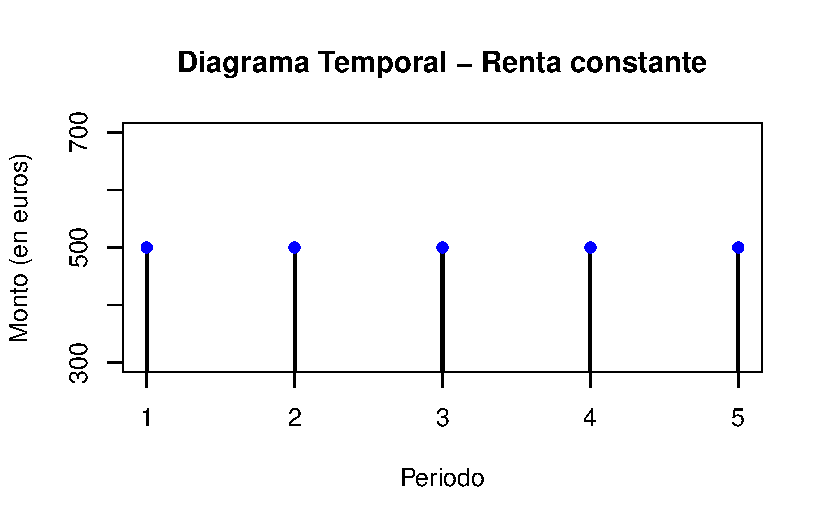
\includegraphics{sesion02_renta_fija_files/figure-pdf/unnamed-chunk-1-1.pdf}

Por ejemplo, una renta mensual de 500 euros durante un período de tiempo
específico. En el diagrama temporal, los pagos se representan mediante
líneas horizontales paralelas.

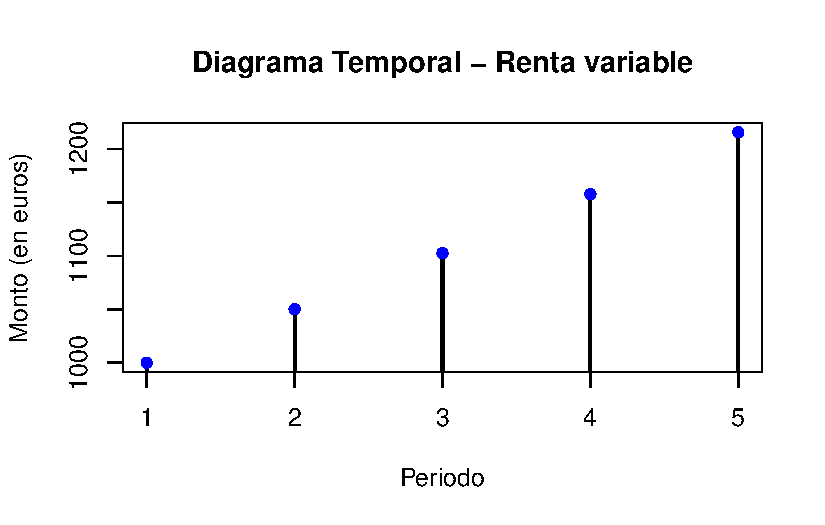
\includegraphics{sesion02_renta_fija_files/figure-pdf/unnamed-chunk-2-1.pdf}

Por ejemplo, una renta que comienza con un pago de 1.000 euros y
experimenta cambios en cada periodo, ya sea en aumento o disminución. En
el diagrama temporal, los pagos se representan mediante líneas que
varían en cada periodo.

\subsection{Cálculos}\label{cuxe1lculos}

Además de clasificar las rentas financieras, es \textbf{fundamental
calcular su valor} actual y final \textbf{en el contexto del interés
compuesto.}

\begin{itemize}
\item
  El \textbf{valor actual} de una renta constante representa la
  \textbf{suma de los pagos descontados en el momento presente},
  considerando una tasa de interés adecuada.
\item
  El \textbf{valor final} de una renta constante se refiere al
  \textbf{monto acumulado al final de la serie de pagos}. Estos cálculos
  se realizan utilizando fórmulas específicas que tienen en cuenta la
  tasa de interés, el monto de los pagos y el número de periodos.
\end{itemize}

Para calcular el valor de una renta y aplicar el concepto de
\textbf{interés compuesto, es habitual trabajar con tipos nominales y
efectivos expresados en diferentes frecuencias (mensual, trimestral,
anual)}. Es fundamental en este sentido \textbf{utilizar el tipo de
interés correspondiente a la frecuencia de los cobros y pagos asociados
a la renta}, a fin de obtener una valoración precisa y realista. Es
decir, que debemos de reflejar adecuadamente la renta en función del
periodo en el que se producen los flujos de caja (términos mensuales,
por ejemplo) y el período del tipo de interés a aplicar (tendrá que ser
mensual en este caso), asegurando así una evaluación precisa y acorde a
la situación.

El valor actual representa la suma de los pagos descontados al presente,
teniendo en cuenta una tasa de interés adecuada.

\begin{tcolorbox}[enhanced jigsaw, toprule=.15mm, left=2mm, arc=.35mm, breakable, bottomrule=.15mm, opacityback=0, rightrule=.15mm, leftrule=.75mm, colframe=quarto-callout-note-color-frame, colback=white]
\begin{minipage}[t]{5.5mm}
\textcolor{quarto-callout-note-color}{\faInfo}
\end{minipage}%
\begin{minipage}[t]{\textwidth - 5.5mm}

La fórmula general para calcular el \textbf{valor actual de una renta
constante} es:

\[V_0=c\cdot\frac{1-\left(1+i\right)^{-n}}{i}\]

Donde,

\begin{itemize}
\item
  \(V_0\), es el valor actual.
\item
  \(C\), es cuota o cuantía.
\item
  \(i\), es el tipo de interés.
\item
  \(n\), es el tiempo transcurrido.
\end{itemize}

\end{minipage}%
\end{tcolorbox}

Por otro lado, el valor final de una renta constante se refiere al monto
acumulado al final de la serie de pagos.

\begin{tcolorbox}[enhanced jigsaw, toprule=.15mm, left=2mm, arc=.35mm, breakable, bottomrule=.15mm, opacityback=0, rightrule=.15mm, leftrule=.75mm, colframe=quarto-callout-note-color-frame, colback=white]
\begin{minipage}[t]{5.5mm}
\textcolor{quarto-callout-note-color}{\faInfo}
\end{minipage}%
\begin{minipage}[t]{\textwidth - 5.5mm}

La fórmula para calcular el \textbf{valor final de una renta constante}
es: \[V_f=c\cdot\frac{\left(1+i\right)^{n}-1}{i}\]

Donde,

\begin{itemize}
\item
  \(V_f\), es el valor final.
\item
  \(C\), es cuota o cuantía.
\item
  \(i\), es el tipo de interés.
\item
  \(n\), es el tiempo transcurrido.
\end{itemize}

Estas fórmulas son fundamentales para calcular el valor actual y final
de una renta constante, lo cual permite evaluar la rentabilidad y
viabilidad de operaciones financieras que involucran flujos de pagos o
cobros periódicos en el tiempo.

\end{minipage}%
\end{tcolorbox}

Las fórmulas presentadas anteriormente son para calcular rentas
postpagables, es decir, en las que los pagos se realizan al final de
cada período. Sin embargo, es posible \textbf{convertir una renta
prepagable}, en la que los pagos se realizan al inicio de cada período,
\textbf{en una renta postpagable cambiando el momento de los pagos}.

\begin{tcolorbox}[enhanced jigsaw, toprule=.15mm, left=2mm, arc=.35mm, breakable, bottomrule=.15mm, opacityback=0, rightrule=.15mm, leftrule=.75mm, colframe=quarto-callout-note-color-frame, colback=white]
\begin{minipage}[t]{5.5mm}
\textcolor{quarto-callout-note-color}{\faInfo}
\end{minipage}%
\begin{minipage}[t]{\textwidth - 5.5mm}

Para una renta constante prepagable, el valor actual se calcula
utilizando la fórmula:

\[V_0=c\cdot\frac{1-\left(1+i\right)^{-n}}{i}\cdot(1+i)^n\]

Y, el valor final:

\[V_f=c\cdot\frac{\left(1+i\right)^{n}-1}{i}\cdot(1+i)^n\]

\end{minipage}%
\end{tcolorbox}

\begin{tcolorbox}[enhanced jigsaw, toprule=.15mm, left=2mm, arc=.35mm, breakable, bottomrule=.15mm, opacityback=0, rightrule=.15mm, leftrule=.75mm, colframe=quarto-callout-warning-color-frame, colback=white]
\begin{minipage}[t]{5.5mm}
\textcolor{quarto-callout-warning-color}{\faExclamationTriangle}
\end{minipage}%
\begin{minipage}[t]{\textwidth - 5.5mm}

\textbf{La diferencia entre ambas fórmulas (perpagables y postpagables)
radica en la presencia del factor} \((1 + i)^n\) en la fórmula de la
renta prepagable. Este factor tiene en cuenta los pagos anticipados
realizados al inicio de cada período, lo cual afecta el valor actual de
la renta.

\end{minipage}%
\end{tcolorbox}

Es importante entender la diferencia entre estos dos tipos de rentas
para poder aplicar las fórmulas correctamente.

Por ejemplo, una \textbf{renta postpagable se aplica a un préstamo} en
el cual se efectúan pagos periódicos después de cada período. En
contraste, una \textbf{renta prepagable se relaciona con un contrato de
alquiler} en el que se realizan pagos anticipados para asegurar el
derecho de disfrute de la propiedad en períodos futuros.

\section{Renta Fija}\label{renta-fija}

\subsection{Concepto}\label{concepto-1}

Un activo de renta fija es un valor que \textbf{representa una deuda
para el emisor} y que tiene una retribución que se fija, generalmente,
por adelantado.

Un activo de renta fija es, por lo tanto, un valor que representa el
derecho a recibir pagos periódicos o al final de la operación,
prefijados y regulares en el futuro.

El emisor de un bono debe seleccionar \textbf{las condiciones} (fecha de
emisión, fecha de vencimiento, tipo de interés, periodicidad de pago,
etc.) que \textbf{una vez fijadas no se pueden modificar. Por ese motivo
este tipo de activos reciben el nombre de renta fija.}

\subsection{Características generales de la renta
fija}\label{caracteruxedsticas-generales-de-la-renta-fija}

Los elementos característicos de un título de renta fija son los
siguientes:

\begin{enumerate}
\def\labelenumi{\arabic{enumi}.}
\item
  \textbf{Tipo de emisor}: es aquel que obtiene la financiación del
  mercado y asume la obligación de pagar los cupones y devolver el
  principal. Puede ser público (administraciones públicas) o privado
  (bancos y empresas).
\item
  \textbf{Valor Nominal} (VN): Monto de la deuda contraída por el emisor
  con el suscriptor, comprador o tenedor del título.
\item
  \textbf{Precio de emisión} (Pe): Precio al que se emite y suscribe el
  título en el mercado primario.
\item
  \textbf{Número de títulos emitidos} (N): Unidades en las que se divide
  el empréstito.
\item
  \textbf{Importe de la emisión} (VN x N): Valor total de la emisión
  calculado multiplicando el valor nominal por el número de títulos
  emitidos.
\item
  \textbf{Fecha de emisión}: Fecha en la que se emite y pone en
  circulación el título de renta fija.
\item
  \textbf{Fecha de vencimiento}: Fecha en la que finaliza la vida del
  título y se debe devolver el valor nominal.
\item
  \textbf{Cupón}: Pago periódico de interés que se calcula como un
  porcentaje del valor nominal del título.
\item
  \textbf{Frecuencia de pago}: Periodo en el que se realiza el pago del
  cupón, que puede ser anual, semestral, al vencimiento, entre otros.
\item
  \textbf{Amortización}: Monto devuelto por el emisor al vencimiento o
  en fechas preestablecidas, generalmente como un porcentaje del valor
  nominal.
\item
  \textbf{Rating}: Calificación crediticia asignada al emisor o a la
  emisión de renta fija, que indica su calidad crediticia y nivel de
  riesgo.
\item
  \textbf{Vencimiento}: fecha en que se termina de repagar la totalidad
  de la deuda. En este momento el bono cesa.
\item
  \textbf{Bono cupón cero}: son aquellos instrumentos, emitidos al
  descuento, que no generan flujos intermedios (no pagan cupones). El
  rendimiento es el obtenido por la diferencia entre el precio de compra
  y el de venta o amortización del título.
\item
  \textbf{TIR}: rendimiento del instrumento a priori, que
  \textbf{dependerá de las condiciones de mercado}. No confundir con el
  cupón con la TIR, ya que el primero es fijo y la segunda dependerá del
  precio al que se adquiera el título.
\item
  \textbf{TRE}: Tasa de Rentabilidad Efectiva o \textbf{rendimiento real
  obtenido después de realizar la inversión}. Se calcula teniendo en
  cuenta los flujos de efectivo reales que se generan durante la vida de
  la inversión, incluyendo los ingresos y los desembolsos de efectivo.
  La rentabilidad efectiva refleja el rendimiento real de la inversión,
  \textbf{teniendo en cuenta cualquier variación en los flujos de
  efectivo y las tasas de interés}.
\end{enumerate}

Estos elementos son importantes para comprender y evaluar los títulos de
renta fija en términos de su emisor, valor, precio, pagos de intereses,
fechas y riesgo crediticio.

\textbf{Según el vencimiento del activo}, los títulos de renta fija se
pueden clasificar en dos categorías:

\begin{enumerate}
\def\labelenumi{\arabic{enumi}.}
\item
  \textbf{Activos monetarios}: Son aquellos activos de renta fija cuyo
  \textbf{vencimiento} en el momento de la emisión se sitúa generalmente
  \textbf{en torno a los dieciocho meses o en plazos inferiores}. Estos
  activos suelen tener un plazo de vencimiento corto y se utilizan para
  cubrir necesidades de financiamiento a corto plazo. Ejemplos de
  activos monetarios son las Letras del Tesoro y los Pagarés de empresa.
\item
  \textbf{Activos del mercado de capitales}: Son activos de renta fija
  cuyo \textbf{vencimiento} en el momento de la emisión es
  \textbf{superior a los dieciocho meses}. Estos activos se emiten en
  plazos más largos y suelen formar parte del mercado de capitales. Los
  plazos típicos para estos activos son 3, 5, 10, 15, 20 y 30 años.
  Ejemplos de activos del mercado de capitales son los Bonos y
  Obligaciones del Estado.
\end{enumerate}

La clasificación \textbf{según el tipo de interés} sería:

Activos con interés \textbf{implícito}:

\begin{itemize}
\tightlist
\item
  Activos \textbf{al descuento}: Son activos en los que el interés o
  rendimiento se obtiene a partir del diferencial entre el precio de
  suscripción o compra y el precio de venta o amortización. En estos
  activos, la amortización se realiza al valor nominal. Los ejemplos
  típicos son las Letras del Tesoro, los Pagarés de Empresa y los Bonos
  Cupón Cero (STRIPS).
\end{itemize}

Activos con interés \textbf{implícito y explícito}:

\begin{itemize}
\item
  Los intereses explícitos que devenga un activo de renta fija se
  denominan cupones.
\item
  Activos \textbf{con prima de emisión}: Son activos en los que el
  interés total se compone tanto del diferencial de amortización o venta
  menos la suscripción o compra, como del pago de cupones periódicos.
  Estos activos \textbf{se emiten a un precio inferior al valor nominal}
  (\textbf{bajo par}).
\item
  Activos \textbf{con prima de reembolso}: Son activos de interés
  explícito en los que el valor de reembolso es superior al valor
  nominal. Además de los cupones periódicos, al vencimiento \textbf{el
  inversor recibirá un monto superior al valor nominal (amortización
  sobre par)}.
\end{itemize}

\subsection{Estructura del mercado de deuda
pública}\label{estructura-del-mercado-de-deuda-puxfablica}

\subsubsection{Activos que se negocian}\label{activos-que-se-negocian}

\textbf{Letras del Tesoro}

\begin{itemize}
\item
  Títulos a corto plazo.
\item
  Emitidos al descuento.
\item
  Representados por anotaciones en cuenta en la Central de Anotaciones
  de BdE.
\item
  La rentabilidad es la diferencia entre el valor nominal y el precio de
  adquisición pagado por el inversor.
\item
  Procedimiento de emisión mediante subasta española.
\end{itemize}

\textbf{Bonos y obligaciones del estado}

\begin{itemize}
\item
  Títulos a largo plazo. Bonos a 3 y 5 años y Obligaciones a 10, 15 y 30
  años.
\item
  Representados por anotaciones en cuenta en la Central de Anotaciones
  de BdE.
\item
  Pagan cupones anuales siendo reembolsables a vencimiento por su valor
  nominal.
\item
  Procedimiento de emisión mediante subasta española.
\end{itemize}

\subsubsection{Miembros del mercado}\label{miembros-del-mercado}

\textbf{El Tesoro}

\begin{itemize}
\item
  Cubrir las necesidades de endeudamiento del Estado al menor coste
  posible.
\item
  Mantener un adecuado grado de liquidez en el mercado.
\item
  Ofrecer a los inversores instrumentos financieros atractivos.
\end{itemize}

\textbf{Banco de España}

\begin{itemize}
\item
  Agente financiero de la deuda pública.
\item
  Gestiona la Central de Anotaciones.
\item
  Supervisa el funcionamiento y la transparencia del mercado de Deuda
  Pública.
\end{itemize}

\textbf{Entidades Gestoras}

\begin{itemize}
\item
  Llevan las cuentas de quienes no están autorizados a operar
  directamente a través de la central de Anotaciones.
\item
  Salvo que sean agencias de valores, pueden ser Titular de Cuenta.
\item
  Realizan funciones registrales, de compensación y liquidación y de
  custodia en relación al mercado de deuda pública.
\end{itemize}

\textbf{Creadores de mercado}

\begin{itemize}
\item
  Entidades financieras cuyo objetivo es favorecer la liquidez del
  mercado secundario.
\item
  Cotizan sistemáticamente precios de compra y de venta y operan con
  unos volúmenes mínimos.
\end{itemize}

\subsubsection{Mercado primario: procedimiento de emisión de los valores
del
Tesoro}\label{mercado-primario-procedimiento-de-emisiuxf3n-de-los-valores-del-tesoro}

El Tesoro español puede emitir Letras del Tesoro, Bonos y Obligaciones
del Estado mediante dos métodos: sindicación u oferta pública.

\subsubsection{Mercado secundario}\label{mercado-secundario}

La negociación en el mercado secundario se puede realizar a través de
varios sistemas

\subsection{Mercado de renta fija
privada}\label{mercado-de-renta-fija-privada}

En el mercado de renta fija privada se utilizan diferentes instrumentos,
como:

\begin{itemize}
\tightlist
\item
  Pagarés de empresa
\item
  Bonos convertibles
\item
  Acciones preferentes
\item
  Fondos de titulización de activos
\end{itemize}

\subsection{Rating}\label{rating}

El \textbf{rating o solvencia crediticia} conocido también como el
\textbf{riesgo de crédito (o de contraparte)}, se mide como la
posibilidad de que el emisor de un bono no pueda hacer frente a los
pagos de los cupones o del principal

Po lo tanto a través del rating podremos \textbf{valorar el nivel de
solvencia de un emisor y sus perspectivas futuras de pago}. El rating
proporciona un indicador de \textbf{referencia del riesgo crediticio}
que soporta el inversor. Esta calificación se realiza por empresas
independientes especializadas en el análisis de riesgos, siendo las
principales Moody ́s, Standard and Poor ́s y Fitch.

Por lo general, \textbf{cuanto mejor sea la calificación crediticia
(rating) de un emisor o de una emisión, menor será la prima de riesgo
del bono y, por lo tanto, menor será su rentabilidad exigida}.

\subsection{Otros riesgos asociados a la renta
fija}\label{otros-riesgos-asociados-a-la-renta-fija}

La \textbf{denominación de ``renta fija'' puede ser engañosa}, ya que
puede dar la impresión de que la rentabilidad está preestablecida y
garantizada. Sin embargo, en realidad, lo que es fijo en una inversión
de renta fija es el conocimiento previo de los montos, las fechas en que
el emisor pagará los cupones y la devolución del principal. Sin embargo,
debido a \textbf{la variación de los tipos de interés en el mercado, el
precio de un título de renta fija puede fluctuar al igual que cualquier
otro activo financiero, subiendo o bajando}.

Los riesgos potenciales asociados a la renta fija son:

• \textbf{Riesgo de precio}

• \textbf{Riesgo de reinversión}

• Riesgo de crédito

• Riesgo de inflación

• Riesgo de tipo de cambio

• Riesgo de amortización anticipada

• Riesgo de liquidez

En esta parte \textbf{nos centraremos en los dos primeros, entendidos
como el riesgo de tipo de interés}:

\begin{itemize}
\item
  El \textbf{riesgo de precio es la principal fuente de incertidumbre} a
  la que se enfrenta un inversor en productos de renta fija. Todos los
  productos de renta fija están sujetos a este riesgo.Ya que
  \textbf{cuando el tipo de interés de mercado sube, el precio del bono
  baja.Y, viceversa}, cuando el tipo de interés de mercado baja, el
  precio del bono sube.
\item
  El \textbf{riesgo de reinversión} aparece en aquellos activos de renta
  fija con rendimiento explícito y se refiere al hecho de que durante el
  transcurso de la vida de un bono, se asume la \textbf{incertidumbre
  sobre la reinversión del importe cobrado del cupón}. El cupón se
  reinvertirá en otro producto de renta fija que tendrá, muy
  probablemente, un tipo de interés superior o inferior al del producto
  en su momento inicial.
\end{itemize}

\subsection{Relación precio-TIR: principios de
Malkiel}\label{relaciuxf3n-precio-tir-principios-de-malkiel}

La relación precio-TIR sigue los principios de Malkiel, que incluyen:

\begin{itemize}
\tightlist
\item
  El valor de un activo de renta fija varía en sentido inverso a su
  rentabilidad.
\item
  Los activos con menor cupón experimentan mayores cambios de valor.
\item
  Un incremento de la TIR supone una caída de precio inferior a la caída
  provocada por una disminución de la TIR.
\end{itemize}

\subsection{Curva y estructura temporal de los tipos de interés
(ETTI)}\label{curva-y-estructura-temporal-de-los-tipos-de-interuxe9s-etti}

\subsubsection{Concepto}\label{concepto-2}

La curva de tipos de interés es una herramienta importante en el mercado
financiero que proporciona información sobre las rentabilidades de los
activos de renta fija en relación con sus vencimientos. La curva se
representa gráficamente trazando los rendimientos de los bonos con
diferentes vencimientos. La estructura temporal de los tipos de interés,
por su parte, muestra los rendimientos de los bonos cupón cero y se
utiliza para analizar la relación entre los tipos de interés y los
vencimientos.

El perfil de la curva de tipos de interés, o de un tramo de ella, puede
ser plano, creciente o decreciente. Un perfil plano indica que los
rendimientos son similares para todos los vencimientos, mientras que un
perfil creciente indica que los rendimientos aumentan a medida que
aumenta el vencimiento. Por el contrario, un perfil decreciente indica
que los rendimientos disminuyen a medida que aumenta el vencimiento.

Es importante tener en cuenta que si hay cambios en las expectativas o
variables relevantes, las curvas de tipos de interés se desplazan y
modifican su perfil. Por ejemplo, si se espera que la inflación aumente,
esto puede provocar un aumento en los tipos de interés a largo plazo y
una pendiente más pronunciada en la curva. En general, la curva de tipos
de interés es una herramienta valiosa para los inversores y analistas
financieros que buscan entender las tendencias del mercado y tomar
decisiones informadas sobre sus inversiones.

\subsubsection{Teorías explicativas de la
ETTI}\label{teoruxedas-explicativas-de-la-etti}

La curva de tipos de interés muestra las rentabilidades de los activos
de renta fija en relación con sus vencimientos. Existen diferentes
teorías que explican cómo se forma la curva. La Teoría de la Preferencia
por la Liquidez establece que la curva debe ser creciente, ya que los
inversores prefieren invertir a corto plazo para poder convertir en
liquidez los activos si es necesario. La Teoría de las Expectativas del
Mercado indica que la curva se forma en función de las expectativas de
los inversores sobre cómo evolucionarán los tipos de interés en el
futuro. Finalmente, la Teoría del Hábitat Preferido sintetiza estas
teorías y establece que la oferta y la demanda de activos financieros
debe ajustar sus plazos según el ``hábitat'' en el que se encuentren,
existiendo primas para aquellos vencimientos donde hay una demanda
insuficiente. En general, estas teorías son útiles para entender las
tendencias del mercado y tomar decisiones informadas sobre las
inversiones.

Un desarrollo más amplio de las teorías explicativas de la estructura
temporal de los tipos de interés (ETTI) sería:

\begin{itemize}
\item
  De la Teoría de la Preferencia por la liquidez, se infiere que la
  curva de rendimientos de una inversión será siempre creciente en
  función del tiempo, ya que en principio un inversor preferirá invertir
  a corto plazo que a largo plazo, al poder conseguir convertir antes en
  liquidez los activos si así le fuera necesario.
\item
  La Teoría de las Expectativas del Mercado, enuncia que la ETTI se
  forma de manera exclusiva en función de las expectativas que tienen
  los potenciales inversores en relación a cómo van a evolucionar los
  tipos de interés en el futuro. Por tanto, la curva sería creciente
  cuando se espere que los tipos vayan a subir debido a que haya por
  ejemplo una elevada inflación, y sería descendente cuando la
  expectativa fuera de bajada de la inflación.
\item
  La Teoría del Hábitat Preferido, por su parte ha tratado de sintetizar
  estas teorías, estableciendo que el equilibrio de mercado obliga a que
  la oferta y la demanda de activos financieros debe ajustar sus plazos
  en cada momento, según el ``hábitat'' en el que nos encontremos,
  existiendo primas para aquellos vencimientos donde hay una demanda
  insuficiente, de tal manera que dichas primas serían las que
  inducirían a los inversores al abandono de sus hábitats preferidos,
  pasando de largo a corto plazo o viceversa.
\end{itemize}

\subsubsection{Ejemplo ETTI}\label{ejemplo-etti}

Si las cotizaciones actuales de los bonos cupón cero a 3,5 y 10 años es
del 100\% y sus valores de reembolso son: 115,76\%, 127,63\% y 162,89\%
respectivamente, ¿cuál será el perfil que adopte la ETTI?

\begin{enumerate}
\def\labelenumi{\alph{enumi}.}
\item
  Positiva.
\item
  Negativa.
\item
  Plana.
\item
  Exponencial.
\end{enumerate}

\begin{tcolorbox}[enhanced jigsaw, toprule=.15mm, left=2mm, arc=.35mm, breakable, bottomrule=.15mm, opacityback=0, rightrule=.15mm, leftrule=.75mm, colframe=quarto-callout-tip-color-frame, colback=white]
\begin{minipage}[t]{5.5mm}
\textcolor{quarto-callout-tip-color}{\faLightbulb}
\end{minipage}%
\begin{minipage}[t]{\textwidth - 5.5mm}

La respuesta \textbf{correcta es la c}.

Para saber que el perfil adoptará la ETTI simplemente deberemos calcular
el valor que toma la TIR de los 3 bonos cupón cero referidos y,
ordenalos en función de su plazo de vencimiento. De forma que si el
precio de un bono cupón cero viene dado por:

\[P_0(\%)=\frac{Reembolso(\%)}{(1+TIR)^{n}}\]

\textbf{BONO 1}

\[100=\frac{115,76}{(1+TIR)^{3}}=>TIR=5\%\]

\textbf{BONO 2}

\[100=\frac{127,63}{(1+TIR)^{5}}=>TIR=5\%\]

\textbf{BONO 3}

\[100=\frac{162,89}{(1+TIR)^{10}}=>TIR=5\%\]

luego, el perfil que adoptará la ETTI será plano ya que para los tres
bonos la tasa interna de rentabilidad \textbf{(TIR) a, 5 y 10 años es
igual al 5\%}.

\end{minipage}%
\end{tcolorbox}

\subsection{Medición y gestión del riesgo de tipo de
interés}\label{mediciuxf3n-y-gestiuxf3n-del-riesgo-de-tipo-de-interuxe9s}

\subsubsection{Sensibilidad}\label{sensibilidad}

La sensibilidad es una \textbf{herramienta} valiosa para determinar cómo
se comportará el precio de un bono ante pequeñas variaciones en la TIR.
Es por tanto, una medida de riesgo en la gestión de activos de renta
fija. Esta medida \textbf{nos indica cuán ``sensible'' es el precio del
bono (en términos absolutos, viene dada en unidades monetarias) a las
fluctuaciones absolutas que se producen en los tipos de interés}.

\begin{itemize}
\item
  En \textbf{escenarios de tipos de interés bajos}, un bono con una
  \textbf{sensibilidad mayor experimentará un aumento de precio más
  significativo} si se produce una variación en la TIR.
\item
  Por otro lado, en \textbf{escenarios de tipos de interés altos}, un
  bono con una \textbf{sensibilidad menor experimentará una disminución
  de precio menor} si hay una variación en la TIR.
\end{itemize}

Sin embargo, como la sensibilidad refleja las variaciones de los precios
en términos absolutos, \textbf{no es adecuada para comparar bonos con
diferentes precios y características}. En este caso, se requiere un
análisis de la duración de los bonos.

Para hallar la sensibilidad (o sensibilidad absoluta) ante cambios en el
precio, calcularemos lo siguiente:

\begin{tcolorbox}[enhanced jigsaw, toprule=.15mm, left=2mm, arc=.35mm, breakable, bottomrule=.15mm, opacityback=0, rightrule=.15mm, leftrule=.75mm, colframe=quarto-callout-note-color-frame, colback=white]
\begin{minipage}[t]{5.5mm}
\textcolor{quarto-callout-note-color}{\faInfo}
\end{minipage}%
\begin{minipage}[t]{\textwidth - 5.5mm}

\begin{enumerate}
\def\labelenumi{\arabic{enumi}.}
\tightlist
\item
  La Duración de Macaulay
\end{enumerate}

\[D=\frac{\sum_{t=1}^{n}\frac{F_t\cdot t}{\left(1+r\right)^t}}{P}\]

\begin{enumerate}
\def\labelenumi{\arabic{enumi}.}
\setcounter{enumi}{1}
\tightlist
\item
  La Duración corregida
\end{enumerate}

\[D_{corregida}=\frac{D}{\left(1+TIR\right)} \]

\begin{enumerate}
\def\labelenumi{\arabic{enumi}.}
\setcounter{enumi}{2}
\tightlist
\item
  La propia sensibilidad
\end{enumerate}

\[S= Duracion\,corregida \cdot \frac{Precio\,entero}{100}\]

Podemos usar la sensibilidad como una aproximación lineal del nuevo
valor de un bono (\(P_1\)) ante una variación absoluta de la TIR
(\(\Delta TIR\)) es:

\[P_1\simeq P_0 + ((-S)\cdot\Delta TIR)\]

\end{minipage}%
\end{tcolorbox}

\subsubsection{Duración}\label{duraciuxf3n}

La \textbf{duración de Macaulay} es una de las características más
importantes que definen un bono. Los gestores de renta fija suelen
utilizar esta medida debido a sus propiedades, ya que \textbf{permite
establecer relaciones fundamentales entre} la estructura de un bono,
\textbf{su TIR y su precio}.

La duración es la media de los periodos de pago de los flujos de un bono
ponderados por el peso que representa el valor actual de los mismos en
el precio del bono.

\begin{tcolorbox}[enhanced jigsaw, toprule=.15mm, left=2mm, arc=.35mm, breakable, bottomrule=.15mm, opacityback=0, rightrule=.15mm, leftrule=.75mm, colframe=quarto-callout-note-color-frame, colback=white]
\begin{minipage}[t]{5.5mm}
\textcolor{quarto-callout-note-color}{\faInfo}
\end{minipage}%
\begin{minipage}[t]{\textwidth - 5.5mm}

Duración de Macaulay (o simplemente Duración)

\[D=\frac{\sum_{t=1}^{n}\frac{F_t\cdot t}{\left(1+r\right)^t}}{P_0}\]

Donde,

\begin{itemize}
\item
  \(D\), Duración de Macaulay expresada en años.
\item
  \(F_t\), Flujos a percibir por la tenencia de un bono (cupón y
  principal).
\item
  \(P_0\), es el precio entero de un bono o valor actual del mismo
  (\(V_0\)).
\item
  \(r\), es la TIR.
\item
  \(t\), es el tiempo hasta el vencimiento de cada uno de los flujos del
  bono.
\end{itemize}

\end{minipage}%
\end{tcolorbox}

Es por lo tanto, una media ponderada de la vida de un bono, es decir, la
``vida media'' del bono. La duración \textbf{se expresa} en unidades
temporales, \textbf{normalmente en años}.

\subsubsection{Propiedades de la
Duración}\label{propiedades-de-la-duraciuxf3n}

De la expresión general para el cálculo de la duración, se puede deducir
que \textbf{un bono cupón cero (un solo flujo en la fecha de
vencimiento) tiene una duración igual a su vencimiento}.

La duración \textbf{puede definirse también como una medida de la
sensibilidad relativa de un bono}. Es decir, relaciona las variaciones
relativas del precio con las variaciones relativas de la TIR.

De forma que también podemos deducir que:

\begin{itemize}
\item
  Ante previsiones de \textbf{subidas en los tipos de interés}, será
  \textbf{más interesante} para el inversor en renta fija invertir en
  \textbf{bonos con una duración pequeña}.
\item
  Ante previsiones de \textbf{bajadas en los tipos de interés}, será
  \textbf{más interesante} para el inversor en renta fija invertir en
  \textbf{bonos con más duración}.
\end{itemize}

Si relacionamos la duración con el vencimiento de un bono, manteniendo
constante la estructura de los flujos y la TIR, podemos afirmar que en
general: a \textbf{mayor plazo de amortización, mayor duración}.

\begin{tcolorbox}[enhanced jigsaw, toprule=.15mm, left=2mm, arc=.35mm, breakable, bottomrule=.15mm, opacityback=0, rightrule=.15mm, leftrule=.75mm, colframe=quarto-callout-important-color-frame, colback=white]
\begin{minipage}[t]{5.5mm}
\textcolor{quarto-callout-important-color}{\faExclamation}
\end{minipage}%
\begin{minipage}[t]{\textwidth - 5.5mm}

Con una \textbf{excepción}: y es que para bonos bajo la par con
vencimientos largos, el incremento de la duración a medida que aumenta
el plazo de amortización, presenta un punto de inflexión a partir del
cual se invierte la tendencia inicial.

\end{minipage}%
\end{tcolorbox}

De la relación entre la duración y la TIR, podemos deducir que:
\textbf{cuando aumenta la TIR, disminuye la duración.}

De la relación entre la duración y la periodicidad de los cupones
podemos extraer la siguiente propiedad: \textbf{a mayor frecuencia en el
pago de cupones menor duración}. Ya que al aumentar la frecuencia en el
pago de cupones disminuye la importancia relativa del último flujo, ya
que el aumento de la frecuencia incrementa el valor actual de los
cupones. Por lo tanto, este efecto se traduce en una disminución de la
duración.

De la relación entre la duración y el paso del tiempo, y siempre que la
TIR permanezca constante, se derivan dos propiedades muy importantes. La
primera es:

\begin{itemize}
\item
  \textbf{Con el transcurso del tiempo}, los plazos de los flujos del
  bono se hacen más pequeños y, por lo tanto, \textbf{la duración
  también disminuye}.
\item
  A \textbf{medida que disminuye la vida pendiente de un bono}, también
  \textbf{disminuye su duración}.
\end{itemize}

\subsubsection{Duración corregida o
modificada}\label{duraciuxf3n-corregida-o-modificada}

Hemos visto, dos medidas que relacionan las variaciones del precio de un
bono con las variaciones de su TIR:

\begin{itemize}
\item
  La \textbf{sensibilidad}, donde la \textbf{relación} se da a través
  \textbf{de magnitudes} \textbf{absolutas}, con lo que existe el
  problema de comparar entre diferentes bonos.
\item
  La \textbf{duración}, donde la \textbf{relación} se realiza a través
  \textbf{de magnitudes relativas}, con lo que es posible la comparación
  para diferentes bonos.
\end{itemize}

En este caso, la problemática se produce en la interpretación económica
de las magnitudes. Recordemos que la duración relaciona la variación
relativa del precio con la variación relativa de la TIR, pero esta
última, no tiene una fácil interpretación económica. Para relacionar los
dos problemas, recurriremos al cálculo de la duración corregida, o
duración modificada.

Matemáticamente su expresión es:

\begin{tcolorbox}[enhanced jigsaw, toprule=.15mm, left=2mm, arc=.35mm, breakable, bottomrule=.15mm, opacityback=0, rightrule=.15mm, leftrule=.75mm, colframe=quarto-callout-note-color-frame, colback=white]
\begin{minipage}[t]{5.5mm}
\textcolor{quarto-callout-note-color}{\faInfo}
\end{minipage}%
\begin{minipage}[t]{\textwidth - 5.5mm}

Duración corregida expresada en años

\[D_{corregida}=\frac{Duracion\,de\, Macaulay}{\left(1+TIR\right)}=\frac{D}{\left(1+TIR\right)} \]

\begin{itemize}
\tightlist
\item
  Si la queremos expresada en porcentaje
\end{itemize}

\[D_{corregida}=\frac{Duracion\,de\, Macaulay}{\left(1+TIR\right)}\cdot\frac{1}{100}\]

\end{minipage}%
\end{tcolorbox}

Cuando hablamos de \textbf{volatilidad de los bonos u obligaciones} nos
estamos refiriendo a la sensibilidad de su precio de mercado con
relación a los cambios que se produzcan en el tipo de interés de mercado
(su rendimiento). Así que l\textbf{a podemos definir como la variación
que se produce en el precio del bono con respecto a un incremento (o
decremento) de cien puntos básicos (1\%) de su rendimiento (TIR) hasta
el vencimiento}.

\begin{tcolorbox}[enhanced jigsaw, toprule=.15mm, left=2mm, arc=.35mm, breakable, bottomrule=.15mm, opacityback=0, rightrule=.15mm, leftrule=.75mm, colframe=quarto-callout-note-color-frame, colback=white]
\begin{minipage}[t]{5.5mm}
\textcolor{quarto-callout-note-color}{\faInfo}
\end{minipage}%
\begin{minipage}[t]{\textwidth - 5.5mm}

Duración corregida para estimar el efecto en precio de variaciones en la
TIR

\[\frac{\Delta P}{P}\simeq  \frac{P_1-P_0}{P_0}\simeq \left(-D_{corregida}\right)\cdot\Delta TIR\]

Alternativamente, la Duración corregida para estimar el efecto en precio
de variaciones en la TIR la podemos expresar como,

\[P_1\simeq P_0\cdot\left[1+((-D_{corregida})\cdot\Delta TIR)\right]\]

Donde,

\begin{itemize}
\item
  \(P_1\), es el precio estimado del bono ante una variación de la TIR.
\item
  \(P_0\), es el precio actual del bono .
\item
  \(D_{corregida}\), es la duración corregida.
\end{itemize}

\end{minipage}%
\end{tcolorbox}

Concretando, el precio de los bonos está inversamente relacionado a su
rendimiento; \textbf{la duración modificada actúa como un multiplicador
dado que cuanto más grande sea, mayor será el impacto en el precio de
los bonos ante un cambio de los tipos de interés}; y, por último, para
una duración modificada determinada, cuánto mayores sean las variaciones
en el tipo de interés, mayor será el porcentaje de cambio en el precio.

\subsubsection{Inmunización}\label{inmunizaciuxf3n}

El riesgo de tipo de interés es uno de los mayores riesgos a los que se
enfrenta un inversor en renta fija, debido a su impacto en el precio y
la reinversión de los cupones. Una subida de los tipos de interés reduce
el valor del activo, mientras que una bajada de los tipos de interés
implica una reinversión de los cupones a tipos más bajos. \textbf{Los
activos con rendimiento implícito no están expuestos al riesgo de
reinversión.}

El horizonte temporal de la inversión es el factor clave que determinará
si el inversor prefiere que los tipos de interés suban o bajen.
\textbf{Si el horizonte temporal es corto, el efecto precio domina y el
inversor preferirá que los tipos de interés bajen. Si el horizonte
temporal es largo, el efecto reinversión es mayor y el inversor
preferirá que los tipos de interés suban.}

Para lograr la \textbf{inmunización}, es importante que la duración y el
horizonte temporal de la inversión estén homogeneizados. La duración de
Macaulay es una medida útil para evaluar la sensibilidad de los precios
de los bonos a los cambios en las tasas de interés. La inmunización
\textbf{se logra haciendo coincidir la duración y el horizonte temporal
de la inversión}, lo que garantiza una rentabilidad mínima igual a la
TIR inicial del bono.

Hay \textbf{tres posibles situaciones} al realizar una inversión:

\begin{itemize}
\item
  Si la \textbf{duración es igual al horizonte temporal, la cartera está
  inmunizada}.
\item
  Si la \textbf{duración es mayor que el horizonte temporal}, el
  inversor deberá vender los activos al final del horizonte temporal y
  asumir un \textbf{riesgo de precio}.
\item
  Si la \textbf{duración es menor que el horizonte temporal}, la
  inversión no estará inmunizada y el inversor deberá hacer una nueva
  inversión asumiendo el \textbf{riesgo de reinversión}.
\end{itemize}

\subsubsection{Resumen de fórmulas}\label{resumen-de-fuxf3rmulas}

\section{Valoración de activos de renta fija a corto y a largo
plazo}\label{valoraciuxf3n-de-activos-de-renta-fija-a-corto-y-a-largo-plazo}

La \textbf{valoración de un bono} se realiza mediante la
\textbf{actualización} de los flujos futuros a las tasas de interés
exigidas por el mercado.

El rendimiento o la \textbf{rentabilidad} de un activo de renta fija
\textbf{se expresa anualmente} a través del régimen de \textbf{interés
simple o} del régimen de interés \textbf{compuesto}.

El régimen de interés \textbf{simple se usará} básicamente para el
cálculo de las rentabilidades de los activos de renta fija a más corto
plazo, es decir, \textbf{para vencimientos inferiores o iguales al año
natural} (Letras del Tesoro y Pagarés de empresa).

Las \textbf{bases de cálculo} establecen la unidad de tiempo a la que se
refiere un tipo de interés determinado. Por extensión se suele llamar
base a la combinación de base y método de cálculo. Las bases más usuales
son: la \textbf{actual y 360 días}.

El régimen de \textbf{interés compuesto} se usará fundamentalmente
\textbf{a través de la TIR} para expresar la rentabilidad de un activo
con interés explícito. También se utilizará para el cálculo del
rendimiento de activos con interés implícito y vencimientos superiores
al año natural.

\textbf{El precio de los bonos y de las obligaciones} (activos de renta
fija a medio y largo plazo) es igual al valor presente de sus flujos de
caja (cash flows) futuros, los cupones y el principal, descontados a un
tipo de interés de mercado.

\begin{longtable}[]{@{}
  >{\raggedright\arraybackslash}p{(\columnwidth - 6\tabcolsep) * \real{0.3014}}
  >{\centering\arraybackslash}p{(\columnwidth - 6\tabcolsep) * \real{0.1918}}
  >{\centering\arraybackslash}p{(\columnwidth - 6\tabcolsep) * \real{0.2740}}
  >{\centering\arraybackslash}p{(\columnwidth - 6\tabcolsep) * \real{0.2329}}@{}}
\toprule\noalign{}
\begin{minipage}[b]{\linewidth}\raggedright
Método
\end{minipage} & \begin{minipage}[b]{\linewidth}\centering
Base
\end{minipage} & \begin{minipage}[b]{\linewidth}\centering
Régimen de interés
\end{minipage} & \begin{minipage}[b]{\linewidth}\centering
Tipo de interés
\end{minipage} \\
\midrule\noalign{}
\endhead
\bottomrule\noalign{}
\endlastfoot
Mercado monetario & Hasta 1 año & Actual/360 & Simple \\
& Más de 1 año & Actual/360 & Compuesto \\
Mercado de capitales & Siempre & Actual/Actual & Compuesto \\
\end{longtable}

Las \textbf{dos formas de expresar el valor de un activo de renta fija},
el valor actual y la TIR, son herramientas importantes en la valoración
y análisis de inversiones en este tipo de activos.

\begin{itemize}
\item
  \textbf{Valor Actual} (\(P_0\)): Se determina aplicando una tasa de
  descuento o tasa esperada de rendimiento al flujo de efectivo esperado
  del activo. Este valor actual representa el precio esperado del
  activo.
\item
  \textbf{Tasa Interna de Rendimiento (TIR)}: Se calcula utilizando el
  precio de mercado del activo o su valor actual. La TIR es la tasa de
  retorno esperada del activo, es decir, la tasa que iguala el valor
  actual del flujo de efectivo del activo con su precio de mercado.
\end{itemize}

Casos particulares en la valoración de un bono:

\begin{enumerate}
\def\labelenumi{\arabic{enumi}.}
\item
  Cálculo del precio de un bono con pago de cupones no anuales:

  \begin{itemize}
  \item
    Se calcula el valor presente de cada cupón teniendo en cuenta el
    plazo y la tasa de descuento adecuada.
  \item
    Se suma el valor presente de los cupones y el valor presente del
    valor nominal para obtener el precio del bono.
  \end{itemize}
\item
  Cálculo del precio de un bono con pago de cupón anual en una fecha
  cualquiera:

  \begin{itemize}
  \item
    Se calcula el tiempo hasta la fecha de pago del cupón y se aplica la
    tasa de descuento correspondiente para obtener el valor presente del
    cupón. Deberemos tener muy en cuenta la fracción de año que falta
    para el pago del primer cupón.
  \item
    Se suma el valor presente de los cupones y el valor presente del
    valor nominal para obtener el precio del bono.
  \end{itemize}
\item
  Cálculo del precio de un bono considerándolo como una renta:

  \begin{itemize}
  \item
    Se calcula el valor presente de los flujos de efectivo generados por
    los cupones y el valor nominal a lo largo de la vida del bono.
    Podemos considerar el pago de cupones periódicos como una renta
    constante, y la amortización del principal, como un bono cupón cero.
  \item
    Se suma el valor presente de los flujos de efectivo para obtener el
    precio del bono.
  \end{itemize}
\item
  Cálculo del precio de un bono cupón cero:

  \begin{itemize}
  \item
    Se calcula el valor presente del valor nominal utilizando el mismo
    procedimiento (actualización de los flujos del bono), sólo que se
    simplifica al calcular el valor actual de un solo flujo.
  \item
    El precio del bono cupón cero es igual al valor presente del valor
    nominal.
  \end{itemize}
\item
  Precio ex-cupón y cupón corrido:

  \begin{itemize}
  \item
    El \textbf{precio ex-cupón} de un bono, es la \textbf{diferencia
    entre el precio entero y el cupón corrido} del bono. \textbf{En la
    mayoría de los mercados} secundarios de renta fija, l\textbf{os
    activos cotizan en precio ex-cupón}.
  \item
    El \textbf{cupón corrido es el interés devengado del próximo cupón}.
    Se calcula como una ponderación simple del próximo cupón.
  \item
    \textbf{El precio entero es lo que efectivamente vale el bono} y,
    por lo tanto, el resultado de la actualización de los flujos del
    bono a la TIR de mercado.
  \end{itemize}
\end{enumerate}

\subsection{Resumen}\label{resumen}

La \textbf{relación} entre el \textbf{precio} de un bono, el
\textbf{cupón y la TIR}

\begin{longtable}[]{@{}
  >{\raggedright\arraybackslash}p{(\columnwidth - 4\tabcolsep) * \real{0.3500}}
  >{\raggedright\arraybackslash}p{(\columnwidth - 4\tabcolsep) * \real{0.3000}}
  >{\raggedright\arraybackslash}p{(\columnwidth - 4\tabcolsep) * \real{0.3500}}@{}}
\toprule\noalign{}
\begin{minipage}[b]{\linewidth}\raggedright
\textbf{Con Prima}
\end{minipage} & \begin{minipage}[b]{\linewidth}\raggedright
\textbf{Emisión de Bonos}
\end{minipage} & \begin{minipage}[b]{\linewidth}\raggedright
\textbf{Con Descuento}
\end{minipage} \\
\midrule\noalign{}
\endhead
\bottomrule\noalign{}
\endlastfoot
Sobre la par & A la Par & Bajo La par \\
Rentabilidad (-) implícita & Rentabilidad = \% Cupón & Rentabilidad (+)
implícita \\
TIR \textless{} Cupón & TIR = Cupón & TIR \textgreater{} Cupón \\
P \textgreater{} VN & P = VN & P \textless{} VN \\
\end{longtable}

\begin{itemize}
\item
  Si el \textbf{precio del bono es igual a su valor nominal, la TIR será
  igual al cupón}. Esto significa que el rendimiento del bono será igual
  al cupón que se paga.
\item
  Si el \textbf{precio del bono es mayor que su valor nominal, la TIR
  será menor} que el cupón.
\item
  Si el \textbf{precio del bono es menor que su valor nominal, la TIR
  será mayor} que el cupón.
\end{itemize}

La relación entre tipos de interés del mercado y los precios de los
bonos

\begin{longtable}[]{@{}lll@{}}
\toprule\noalign{}
TIPOS & PRECIO & TIR \\
\midrule\noalign{}
\endhead
\bottomrule\noalign{}
\endlastfoot
Si ↑ t/ i & ↓ Precio bono & ↑ TIR \\
Si ↓ t/ i & ↑ Precio bono & ↓ TIR \\
\end{longtable}

\begin{tcolorbox}[enhanced jigsaw, toprule=.15mm, left=2mm, arc=.35mm, breakable, bottomrule=.15mm, opacityback=0, rightrule=.15mm, leftrule=.75mm, colframe=quarto-callout-important-color-frame, colback=white]
\begin{minipage}[t]{5.5mm}
\textcolor{quarto-callout-important-color}{\faExclamation}
\end{minipage}%
\begin{minipage}[t]{\textwidth - 5.5mm}

Para hacer la \textbf{valoración} de activos de renta fija, en la
mayoría de casos, y especialmente cuando tengan cupón corrido,
utilizamos la \textbf{CALCULADORA FINCIERA CASIO FC 200V}

\begin{itemize}
\item
  \textbf{Precio/TIR/CC} =\textgreater{} CASIO FC 200V \textbf{(función
  BOND)}
\item
  \textbf{TRE} =\textgreater{} calculamos \textbf{sin emplear ninguna
  función} financiera
\end{itemize}

\end{minipage}%
\end{tcolorbox}

Descripción de los \textbf{distintos precios de los bonos cuando hay
cupón corrido}:

\begin{enumerate}
\def\labelenumi{\arabic{enumi}.}
\item
  Precio \textbf{Entero}: Es el precio cotizado en el mercado para un
  bono, incluyendo el valor del cupón corrido.
\item
  Precio \textbf{Sucio}: También conocido como ``Precio Ex cupón'', es
  el precio de un bono sin incluir el valor del cupón corrido. Es el
  precio al que se negocia el bono en el mercado secundario sin tener en
  cuenta los intereses acumulados.
\item
  Precio \textbf{Efectivo}: Es el precio limpio del bono, es decir, el
  precio sin incluir el valor del cupón corrido.
\end{enumerate}

\textbf{Analíticamente} y con los \textbf{distintos nombres} que podemos
encontrar, tenemos:

\begin{longtable}[]{@{}ll@{}}
\toprule\noalign{}
\endhead
\bottomrule\noalign{}
\endlastfoot
\textbf{NOMBRE} & \textbf{COMPOSICIÓN} \\
Precio \textbf{Entero} = & Precio cotización + Cupón Corrido \\
Precio \textbf{Sucio} = & Precio Ex cupón + Cupón Corrido \\
Precio \textbf{Efectivo} = & Precio Limpio + Cupón Corrido \\
\end{longtable}

\textbf{En la calculadora Casio FC 200V, las variables se definen
mediante:}

\begin{longtable}[]{@{}ll@{}}
\toprule\noalign{}
\textbf{VARIABLE} & \textbf{TRADUCCIÓN} \\
\midrule\noalign{}
\endhead
\bottomrule\noalign{}
\endlastfoot
PRC & Precio ex cupón, limpio o de cotización \\
INT & Cupón corrido \\
CTS & Precio entero, sucio o coste efectivo \\
\end{longtable}

\subsection{Cálculos}\label{cuxe1lculos-1}

\begin{tcolorbox}[enhanced jigsaw, toprule=.15mm, left=2mm, arc=.35mm, breakable, bottomrule=.15mm, opacityback=0, rightrule=.15mm, leftrule=.75mm, colframe=quarto-callout-note-color-frame, colback=white]
\begin{minipage}[t]{5.5mm}
\textcolor{quarto-callout-note-color}{\faInfo}
\end{minipage}%
\begin{minipage}[t]{\textwidth - 5.5mm}

Tipos de interés spot y forward

\begin{itemize}
\tightlist
\item
  Para periodos \textbf{inferiores al año}, capitalización
  \textbf{simple} (a 6 meses dentro de 6):
\end{itemize}

\[(1+_{0}S_{12} \cdot \frac{12 }{12 })=(1+_{0}S_{6} \cdot \frac{6 }{12 })\cdot(1+f_{6,12}\cdot \frac{6 }{12 })\]

\begin{itemize}
\tightlist
\item
  Para periodos \textbf{superiores al año}, capitalización
  \textbf{compuesta} (a 1 año dentro de un año):
\end{itemize}

\[(1+_{0}S_{2})^{2}=(1+_{0}S_{1})^1\cdot(1+f_{1,2})^1\] Donde,

\begin{itemize}
\item
  \(_{0}S_{1}\), es el tipo spot o de contado; el subíndice que aparece
  a la derecha nos indica el momento en que dicho interés está vigente
  y, el de la derecha, el número de periodos de vigencia.
\item
  \(f_{1,2}\), es el tipo forward obtenido a partir de los tipos spot;
  el subíndice nos indica el periodo en que dicho interés estará
  vigente.
\end{itemize}

\href{https://monografia-tipos-spot-forward.netlify.app/}{\textbf{Ejercicios
para practica los tipos de interés implícitos o forward}}

\end{minipage}%
\end{tcolorbox}

\begin{tcolorbox}[enhanced jigsaw, toprule=.15mm, left=2mm, arc=.35mm, breakable, bottomrule=.15mm, opacityback=0, rightrule=.15mm, leftrule=.75mm, colframe=quarto-callout-note-color-frame, colback=white]
\begin{minipage}[t]{5.5mm}
\textcolor{quarto-callout-note-color}{\faInfo}
\end{minipage}%
\begin{minipage}[t]{\textwidth - 5.5mm}

Precio de un activo de Renta Fija (interés implícito)

\begin{itemize}
\tightlist
\item
  \textbf{Mercado monetario (Hasta 1 año, capitalización simple)}
\end{itemize}

\[P_0=\frac{100}{\left(1+i\cdot\frac{Actual}{360}\right)}\]

\begin{itemize}
\tightlist
\item
  \textbf{Mercado monetario (Más de 1 año, capitalización compuesta)}
\end{itemize}

\[P_0=\frac{100}{(1+i)^{Actual/360}}\]

donde,

\begin{itemize}
\item
  \(P_0\), es el precio del activo, expresado en porcentaje sobre el
  nominal.
\item
  \(i\), es el tipo de interés.
\item
  \(Actual\), es el número de días que ha mantenido el inversor el
  activo en su poder.
\end{itemize}

\end{minipage}%
\end{tcolorbox}

\begin{tcolorbox}[enhanced jigsaw, toprule=.15mm, left=2mm, arc=.35mm, breakable, bottomrule=.15mm, opacityback=0, rightrule=.15mm, leftrule=.75mm, colframe=quarto-callout-note-color-frame, colback=white]
\begin{minipage}[t]{5.5mm}
\textcolor{quarto-callout-note-color}{\faInfo}
\end{minipage}%
\begin{minipage}[t]{\textwidth - 5.5mm}

Precio de un activo de Renta Fija (interés explícito)

\[P_0=\frac{C_1}{(1+TIR)}+\frac{C_2}{(1+TIR)^2}+\ ... \ +\frac{C_t}{(1+TIR)^t}\]

Donde,

\begin{itemize}
\item
  \(P_o\), es el precio o valor actual
\item
  \(C_t\), es el cupón en el momento \(t\)
\item
  \(TIR\), es la tasa de descuento o TIR
\end{itemize}

\end{minipage}%
\end{tcolorbox}

La Tasa Interna de Rentabilidad (TIR) es una medida de rentabilidad a
priori que estima anticipadamente el rendimiento de una inversión. Se
calcula considerando los flujos de efectivo futuros y el desembolso
inicial de la inversión. La TIR asume que los flujos de efectivo se
reinvierten a una tasa constante y se basa en la suposición de una curva
de tipos de interés plana.

\begin{tcolorbox}[enhanced jigsaw, toprule=.15mm, left=2mm, arc=.35mm, breakable, bottomrule=.15mm, opacityback=0, rightrule=.15mm, leftrule=.75mm, colframe=quarto-callout-note-color-frame, colback=white]
\begin{minipage}[t]{5.5mm}
\textcolor{quarto-callout-note-color}{\faInfo}
\end{minipage}%
\begin{minipage}[t]{\textwidth - 5.5mm}

Tasa de rentabilidad efectiva (TRE, o rentabilidad efectiva o a
posteriori)

\[P_f=P_0 \cdot \left(1+{TRE}\right)^t\]

Donde,

\begin{itemize}
\item
  \(P_f\), es el precio final o valor final
\item
  \(P_o\), es el precio o valor actual
\item
  \(TRE\), es la rentabilidad efectiva o TRE
\end{itemize}

\end{minipage}%
\end{tcolorbox}

Por otro lado, la Tasa de Rentabilidad Efectiva (TRE) es el
\textbf{rendimiento real obtenido después de realizar la inversión}. Se
calcula teniendo en cuenta los flujos de efectivo reales que se generan
durante la vida de la inversión, incluyendo los ingresos y los
desembolsos de efectivo. La rentabilidad efectiva refleja el rendimiento
real de la inversión, \textbf{teniendo en cuenta cualquier variación en
los flujos de efectivo y las tasas de interés}.

\textbf{Cada una de estas medidas de rentabilidad tiene su utilidad} y
se utiliza en diferentes etapas de la evaluación y seguimiento de una
inversión de Renta Fija. \textbf{La TIR es útil para estimar} el
rendimiento potencial de una inversión antes de realizarla, mientras que
\textbf{la rentabilidad efectiva proporciona una medida más precisa del
rendimiento real después de la inversión}.

Ambas medidas son importantes para tomar decisiones informadas sobre
inversiones y evaluar su desempeño ya que, \textbf{en la medida en que
el tipo de interés al que se podrán reinvertir los cupones no coincida
con la TIR, su rentabilidad efectiva (TRE) en el vencimiento diferirá de
esa TIR}.

El \textbf{cupón corrido} representa el valor proporcional del próximo
pago de cupón que se paga al comprador del bono si la fecha de compra es
posterior a la fecha de pago del cupón anterior.

\begin{tcolorbox}[enhanced jigsaw, toprule=.15mm, left=2mm, arc=.35mm, breakable, bottomrule=.15mm, opacityback=0, rightrule=.15mm, leftrule=.75mm, colframe=quarto-callout-note-color-frame, colback=white]
\begin{minipage}[t]{5.5mm}
\textcolor{quarto-callout-note-color}{\faInfo}
\end{minipage}%
\begin{minipage}[t]{\textwidth - 5.5mm}

Cálculo del cupón corrido

\[CC=\frac{D_c}{D_t}\cdot C\]

Donde,

\begin{itemize}
\item
  \(CC\), es el cupón corrido.
\item
  \(D_{c}\), es el tiempo, en días, transcurrido desde el pago del
  último cupón.
\item
  \(D_{t}\), es el tiempo, en días, que transcurre entre el pago de dos
  cupones consecutivos (días totales de devengo del cupón).
\item
  \(C\), es el importe del cupón que se paga periódicamente.
\end{itemize}

\end{minipage}%
\end{tcolorbox}

\subsection{Ejemplos de valoración}\label{ejemplos-de-valoraciuxf3n}

\begin{enumerate}
\def\labelenumi{\arabic{enumi}.}
\tightlist
\item
  Un bono cupón cero adquirido por 88,333\%, con vencimiento a 4 años.
  ¿Indique cuál de las siguientes afirmaciones es correcta?:
\end{enumerate}

\begin{enumerate}
\def\labelenumi{\alph{enumi}.}
\item
  Su TIR es del 3,15\%
\item
  La TRE es del 3,15\%
\item
  La rentabilidad acumulada al vencimiento es del 11,667\%
\item
  Todas las respuestas son correctas.
\end{enumerate}

\begin{tcolorbox}[enhanced jigsaw, toprule=.15mm, left=2mm, arc=.35mm, breakable, bottomrule=.15mm, opacityback=0, rightrule=.15mm, leftrule=.75mm, colframe=quarto-callout-note-color-frame, colback=white]
\begin{minipage}[t]{5.5mm}
\textcolor{quarto-callout-note-color}{\faInfo}
\end{minipage}%
\begin{minipage}[t]{\textwidth - 5.5mm}

Calculamos la TIR del bono como un descuento en capitalización
compuesta:

\[P_0=\frac{100\ (reembolso \ del  \ 100\%)}{\left(1+TIR\right)^n}\] de
forma que, \[88,333=\frac{100}{\left(1+TIR\right)^4}\]

si resolvemos por la TIR, tenemos

\[TIR=0.0315(3,15\%)\]

En el caso de la TRE, empleamos su fórmula,

\[C_4=C _0\cdot (1+TRE)^4\] al sustitur

\[100=88.333\cdot (1+TRE)^4\] tenemos que

\[TRE=0.0315(3,15\%)\]

\textbf{La TIR coincidirá con la TRE ya que no hay flujos de caja} que
hayan de ser reinvertidos. De forma que el \textbf{riesgo}, derivado de
la \textbf{incertidumbre sobre el tipo de interés}, al que se
reinvertirán los cupones, \textbf{se elimina} ya que se aplica la TIR
desde el inicio de la inversión y hasta el final de la misma:

\[TIR=TRE=0.0315(3,15\%)\]

Finalmente, calculamos la rentabilidad acumulada del periodo como:

\[r_{\left(acumulada\:a\:vencimiento\right)}=100\%-88.333\%=11.667\%\]

\end{minipage}%
\end{tcolorbox}

\begin{enumerate}
\def\labelenumi{\arabic{enumi}.}
\setcounter{enumi}{1}
\tightlist
\item
  El 19 de noviembre de 2016 se compra un bono que vence, exactamente,
  dentro de tres años. Hemos pagado un 102,35\% de su nominal, con una
  TIR del 4,39\% y paga un cupón anual del 5,25\%. Si el inversor tiene
  una política de reinversión de los dividendos y teniendo en cuenta el
  siguiente esquema de tipos de interés para depósitos a un año, ¿cuál
  es la tasa de rentabilidad efectiva (TRE) de esta inversión a la fecha
  de vencimiento?
\end{enumerate}

\begin{longtable}[]{@{}ll@{}}
\toprule\noalign{}
Años & Tipos de interés para depósitos a un año \\
\midrule\noalign{}
\endhead
\bottomrule\noalign{}
\endlastfoot
19-11-17 & 3,00\% \\
19-11-18 & 2,25\% \\
19-11-19 & 1,25\% \\
\end{longtable}

a. 4,30\%

b. 4,42\%

c. 4,25\%

d. Ninguna de las anteriores.

\begin{tcolorbox}[enhanced jigsaw, toprule=.15mm, left=2mm, arc=.35mm, breakable, bottomrule=.15mm, opacityback=0, rightrule=.15mm, leftrule=.75mm, colframe=quarto-callout-note-color-frame, colback=white]
\begin{minipage}[t]{5.5mm}
\textcolor{quarto-callout-note-color}{\faInfo}
\end{minipage}%
\begin{minipage}[t]{\textwidth - 5.5mm}

Recordemos que la Tasa de Rentabilidad Efectiva (TRE) se define como
aquella rentabilidad media anual que tiene en cuenta las tasas de
reinversión de los ingresos de una operación, medida mediante
capitalización compuesta. Y su expresión es la siguiente:

\[V_f=V_0\left(1+i_{TRE}\right)^n\]

De forma que necesitaremos el valor final de la inversión (que lo
calculamos), el valor inicial o precio (es un dato en este caso). De
manera, que para hallar cual será el valor al final de la inversión
teniendo en cuenta la reinversión a los tipos que nos dan, calculamos
primero todos los flujos, esto es, de las cuatro inversiones realizadas:

\[V_f=5.25\left(1+0.03\right)\left(1+0.0225\right)+5.25\left(1+0.0225\right)+105.25\]
\[V_f=116.14729\]

Una vez que ya conocemos el valor final \(V_f\) y el valor inicial
\(V_0\), planteamos la fórmula de la TRE y resolvemos por el tipo de
interés \(i_{TRE}\):

\[V_f=V_0\left(1+i_{TRE}\right)^n\]

Donde,

\[i_{TRE}=\left(\frac{V_f }{V_0}\right)^{\frac{1 }{n }}-1\]

Que al sustituir y calcular, obtenemos un resultado de:

\[i_{TRE}=\left(\frac{116.14729}{102.35}\right)^{\frac{1}{3}}-1=0.04305(4.3\%)\]

\end{minipage}%
\end{tcolorbox}

\begin{enumerate}
\def\labelenumi{\arabic{enumi}.}
\setcounter{enumi}{2}
\tightlist
\item
  Si 1 de marzo de 2025 se compró un bono con cupón del 4,25\% emitido
  el 1 de marzo de 2024 que vence el 28 de febrero de 2028. Si en
  activos similares el mercado se mueve en rentabilidades del 3,50\% el
  precio en porcentaje sobre el nominal es aproximadamente:
\end{enumerate}

\begin{enumerate}
\def\labelenumi{\alph{enumi}.}
\item
  100\%
\item
  100,75\%
\item
  102,11\%
\item
  102.75\%
\end{enumerate}

\begin{tcolorbox}[enhanced jigsaw, toprule=.15mm, left=2mm, arc=.35mm, breakable, bottomrule=.15mm, opacityback=0, rightrule=.15mm, leftrule=.75mm, colframe=quarto-callout-note-color-frame, colback=white]
\begin{minipage}[t]{5.5mm}
\textcolor{quarto-callout-note-color}{\faInfo}
\end{minipage}%
\begin{minipage}[t]{\textwidth - 5.5mm}

En este caso nos piden calcular el precio, pero NO indica de qué precio
se trata, si es el precio entero (o sucio), o por el contrario el precio
excupón (o de cotización); luego eso puede generar dudas. No obstante,
si nos fijamos en este caso concreto a pesar de darnos fechas concretas
(y NO términos) ambos precios coinciden (PS=PL), ya que \textbf{no
existe cupón corrido} debido a que la adquisición del título se lleva a
cabo justo en el momento del pago del 1 er cupón (1).

Por otra parte, hay que recordar que \textbf{se coge la fecha de compra
para el cálculo}, y NO la fecha de emisión \ldots ya que no se adquiere
en la emisión como ya se ha comentado, sino que es adquirido justo al
finalizar el primer año (comienzo del segundo año). Luego si lo
resolvemos con la \textbf{calculadora financiera Casio FC200V} tenemos
que:

\begin{itemize}
\item
  Función: ``BOND''
\item
  SET: ``Annu/Date''
\item
  d1 = 01032025+ EXE
\item
  d2 = 28022028 + EXE
\item
  RDV = 100 + EXE
\item
  CPN = 4,25 + EXE
\item
  PRC = 0 + EXE
\item
  YLD = 3,5\% + EXE
\end{itemize}

Ahora, con el cursor, volvemos sobre ``PRC'' y pulsamos ``SOLVE''.

Resultado:

\begin{itemize}
\item
  PRC = - 102,11\% (precio: excupón, o de cotización)
\item
  INT = - 0,00 (cupón corrido)
\item
  CTS = - 102,11\% (\textbf{precio entero o sucio})
\end{itemize}

\end{minipage}%
\end{tcolorbox}

\begin{enumerate}
\def\labelenumi{\arabic{enumi}.}
\setcounter{enumi}{3}
\tightlist
\item
  Sea una emisión de pagarés a 18 meses con precio de emisión de 43.937
  euros y 50.000 euros de valor nominal. Si seis meses después los
  pagares cotizan a 45.000 euros, ¿cuál es el tipo de interés al que
  están cotizando los pagarés en este momento?
\end{enumerate}

\begin{enumerate}
\def\labelenumi{\alph{enumi}.}
\item
  9\%.
\item
  Menor del 9\%.
\item
  Superior al 9\%.
\item
  No puede saberse con estos datos.
\end{enumerate}

\begin{tcolorbox}[enhanced jigsaw, toprule=.15mm, left=2mm, arc=.35mm, breakable, bottomrule=.15mm, opacityback=0, rightrule=.15mm, leftrule=.75mm, colframe=quarto-callout-note-color-frame, colback=white]
\begin{minipage}[t]{5.5mm}
\textcolor{quarto-callout-note-color}{\faInfo}
\end{minipage}%
\begin{minipage}[t]{\textwidth - 5.5mm}

La respuesta \textbf{correcta es la c}.

Con los datos del enunciado,

\begin{itemize}
\item
  \(P_0=45000\)
\item
  \(Nominal= 50000\)
\item
  \(n=12 \ meses\)
\end{itemize}

y la fórmula del precio de un pagaré/letra,

\[P_o=\frac{N}{\left(1+i\cdot \frac{n}{12}\right)}\] bastará con
susutituir y despejar el tipo de interés implícito,

\[45000=\frac{50000}{\left(1+x\cdot \frac{12}{12}\right)}\] para obtener
tipo de interés al que están cotizando los pagarés en este momento

\[i=0.1111(11,11\%)\]

\end{minipage}%
\end{tcolorbox}

\begin{enumerate}
\def\labelenumi{\arabic{enumi}.}
\setcounter{enumi}{4}
\tightlist
\item
  ¿Cuál es el precio de una Letra del Tesoro comprada en el mercado
  secundario con un tipo de interés implícito del 2,066\% y faltando 225
  días para su vencimiento?
\end{enumerate}

\begin{enumerate}
\def\labelenumi{\alph{enumi}.}
\item
  98,725\%.
\item
  98,505\%.
\item
  98,630\%.
\item
  98,850\%.
\end{enumerate}

\begin{tcolorbox}[enhanced jigsaw, toprule=.15mm, left=2mm, arc=.35mm, breakable, bottomrule=.15mm, opacityback=0, rightrule=.15mm, leftrule=.75mm, colframe=quarto-callout-note-color-frame, colback=white]
\begin{minipage}[t]{5.5mm}
\textcolor{quarto-callout-note-color}{\faInfo}
\end{minipage}%
\begin{minipage}[t]{\textwidth - 5.5mm}

La respuesta \textbf{correcta es la a}.

Empleamos la fórmula del precio de una letra, en capitalización simple y
base 360:

\[P_0=\frac{100}{\left(1+i\cdot \frac{d}{360}\right)}\]

donde al sustituir y calcular

\[P_0=\frac{100}{\left(1+\:0.02066\cdot \frac{225}{360}\right)}\]
tenemos un resultado de

\[P_0=98.725\% \]

\end{minipage}%
\end{tcolorbox}

\begin{enumerate}
\def\labelenumi{\arabic{enumi}.}
\setcounter{enumi}{5}
\tightlist
\item
  ¿Cuál es el precio entero (precio efectivo) de un bono del Estado el
  día 18/12/2021, sabiendo que su cotización (precio ex cupón) es
  101,275\%, que paga cupones constantes anuales del 3,20\% y que su
  vencimiento es el 31/1/2025?
\end{enumerate}

\begin{enumerate}
\def\labelenumi{\alph{enumi}.}
\item
  101,661\%
\item
  98,461\%
\item
  101,275\%
\item
  104,089\%
\end{enumerate}

\begin{tcolorbox}[enhanced jigsaw, toprule=.15mm, left=2mm, arc=.35mm, breakable, bottomrule=.15mm, opacityback=0, rightrule=.15mm, leftrule=.75mm, colframe=quarto-callout-note-color-frame, colback=white]
\begin{minipage}[t]{5.5mm}
\textcolor{quarto-callout-note-color}{\faInfo}
\end{minipage}%
\begin{minipage}[t]{\textwidth - 5.5mm}

Para resolver esta pregunta hemos de calcular el cupón corrido y sumarlo
a su precio de cotización (o precio ex cupón) que es conocido e igual a
101,275\%. Por tanto, planteamos la fórmula del cupón corrido,

\[CC=\frac{D_c}{D_t}\cdot C\]

donde,

\begin{itemize}
\item
  \(CC\), es el cupón corrido.
\item
  \(D_{c}\), es el tiempo transcurrido desde el pago del último cupón.
\item
  \(D_{t}\), es el tiempo que transcurre entre el pago de dos cupones
  consecutivos
\item
  \(C\), es el importe del cupón que se paga periódicamente.
\end{itemize}

Ahora debemos realizar el cálculo para conocer el tiempo (en días) que
ha transcurrido desde el pago del último cupón hasta la fecha presente
(18/12/2021), y para ello sabemos que la próxima fecha del cupón que se
paga periódicamente es el 31/1/2022 (ya que el vencimiento es el
31/1/2025).

Por tanto calculamos su diferencia, sabiendo que desde el 18/12/2021 al
31/1/2022 van 43 días más el día corriente. Es decir 44 días, luego
habrán transcurrido un total de 321 días (365-44) desde que se cobrara
el último cupón.

Lo que implica que el cupón devengado y no cobrado es un rendimiento
implícito que acumula este bono a la fecha de su valoración.

Ahora sustituimos en la fórmula y calculamos,

\[CC=\frac{321}{365}\cdot 0.032=0.02814(2.82\%)\] Luego, el precio
efectivo será la suma del precio ex cupón más el cupón corrido,

\[P_{efectivo}=101.275\%+2.814\%=104.089\%\]

\end{minipage}%
\end{tcolorbox}

\begin{center}\rule{0.5\linewidth}{0.5pt}\end{center}

\section{🧾 Fiscalidad de los rendimientos de renta
fija}\label{fiscalidad-de-los-rendimientos-de-renta-fija}

En el caso de personas físicas, los \textbf{rendimientos generados por
activos de renta fija}, ya sean \textbf{explícitos} (intereses o
cupones) o \textbf{implícitos} (rendimiento generado en el reembolso o
transmisión), se consideran \textbf{rendimientos del capital mobiliario}
y se integran en la \textbf{base imponible del ahorro} del IRPF.

\begin{itemize}
\tightlist
\item
  Los \textbf{rendimientos explícitos} tributan por el importe íntegro
  percibido (por ejemplo, intereses o cupones).
\item
  Los \textbf{rendimientos implícitos} tributan por la
  \textbf{diferencia entre el valor de transmisión o reembolso y el
  valor de adquisición}, teniendo en cuenta los gastos inherentes a la
  operación.
\end{itemize}

La \textbf{tributación de estos rendimientos se realiza conforme a una
escala progresiva} aplicable a la base liquidable del ahorro, que
detallamos a continuación.

\begin{tcolorbox}[enhanced jigsaw, toprule=.15mm, left=2mm, breakable, opacitybacktitle=0.6, toptitle=1mm, coltitle=black, arc=.35mm, leftrule=.75mm, bottomtitle=1mm, titlerule=0mm, title=\textcolor{quarto-callout-tip-color}{\faLightbulb}\hspace{0.5em}{Retención en origen}, rightrule=.15mm, opacityback=0, bottomrule=.15mm, colback=white, colframe=quarto-callout-tip-color-frame, colbacktitle=quarto-callout-tip-color!10!white]

Los rendimientos del capital mobiliario están sujetos a una
\textbf{retención a cuenta del 19\,\%}.\\
\textbf{Excepciones}:

\begin{itemize}
\tightlist
\item
  En el caso de las \textbf{Letras del Tesoro}, no se aplica retención.
\item
  En la \textbf{venta de valores de renta fija antes del vencimiento},
  los intereses devengados (cupones corridos) sí están sujetos a
  retención.
\end{itemize}

\end{tcolorbox}

\begin{center}\rule{0.5\linewidth}{0.5pt}\end{center}

\subsection{💰 Gravamen de la base liquidable del
ahorro}\label{gravamen-de-la-base-liquidable-del-ahorro}

\textbf{Normativa aplicable:} Artículo 66.2 de la Ley del IRPF.

A la \textbf{base liquidable del ahorro} se le aplicará la siguiente
\textbf{escala progresiva}. Esta estructura combina \textbf{cuotas fijas
acumuladas} con un \textbf{tipo marginal} sobre el exceso en cada tramo:

\begin{tcolorbox}[enhanced jigsaw, toprule=.15mm, left=2mm, breakable, opacitybacktitle=0.6, toptitle=1mm, coltitle=black, arc=.35mm, leftrule=.75mm, bottomtitle=1mm, titlerule=0mm, title=\textcolor{quarto-callout-note-color}{\faInfo}\hspace{0.5em}{Escala estatal del ahorro (IRPF)}, rightrule=.15mm, opacityback=0, bottomrule=.15mm, colback=white, colframe=quarto-callout-note-color-frame, colbacktitle=quarto-callout-note-color!10!white]

\begin{longtable}[]{@{}
  >{\raggedright\arraybackslash}p{(\columnwidth - 6\tabcolsep) * \real{0.2126}}
  >{\raggedright\arraybackslash}p{(\columnwidth - 6\tabcolsep) * \real{0.2677}}
  >{\raggedright\arraybackslash}p{(\columnwidth - 6\tabcolsep) * \real{0.3543}}
  >{\raggedright\arraybackslash}p{(\columnwidth - 6\tabcolsep) * \real{0.1654}}@{}}
\toprule\noalign{}
\begin{minipage}[b]{\linewidth}\raggedright
Base liquidable hasta (€)
\end{minipage} & \begin{minipage}[b]{\linewidth}\raggedright
Incremento en cuota íntegra (€)
\end{minipage} & \begin{minipage}[b]{\linewidth}\raggedright
Resto base liquidable del ahorro hasta (€)
\end{minipage} & \begin{minipage}[b]{\linewidth}\raggedright
Tipo aplicable (\%)
\end{minipage} \\
\midrule\noalign{}
\endhead
\bottomrule\noalign{}
\endlastfoot
0 & 0 & 6.000 & 19 \\
6.000,00 & 1.140 & 44.000 & 21 \\
50.000,00 & 10.380 & 150.000 & 23 \\
200.000,00 & 44.880 & 100.000 & 27 \\
300.000,00 & 71.880 & En adelante & 28 \\
\end{longtable}

\end{tcolorbox}

\subsection{🧮 Cálculo de la cuota íntegra del
ahorro}\label{cuxe1lculo-de-la-cuota-uxedntegra-del-ahorro}

El cálculo se realiza aplicando una \textbf{cuota fija acumulada} más un
\textbf{porcentaje marginal} sobre el exceso dentro del tramo
correspondiente.

\textbf{Ejemplo:} Si la base liquidable del ahorro es de
\textbf{250.000,00\,€}, se encuentra en el cuarto tramo, y el cálculo
sería:

\[
\text{Cuota íntegra} = 44.880 + (250.000 - 200.000) \times 0,27
\]

\[
\text{Cuota íntegra} = 44.880 + 50.000 \times 0,27 = 44.880 + 13.500 = 58.380
\]

\section{Ejercicios tipo test}\label{ejercicios-tipo-test}

\begin{enumerate}
\def\labelenumi{\arabic{enumi}.}
\tightlist
\item
  Si la duración de una cartera de renta fija es de 6,5 y el horizonte
  temporal del inversor es de 5 años, podemos afirmar que:
\end{enumerate}

\begin{enumerate}
\def\labelenumi{\alph{enumi}.}
\item
  Nada de ello puede inferirse
\item
  El inversor está asumiendo un menor riesgo de precio con relación a
  una cartera perfectamente inmunizada.
\item
  La cartera esta perfectamente inmunizada.
\item
  Para inmunizar es necesario reducir la duración de la cartera.
\end{enumerate}

\begin{tcolorbox}[enhanced jigsaw, toprule=.15mm, left=2mm, arc=.35mm, breakable, bottomrule=.15mm, opacityback=0, rightrule=.15mm, leftrule=.75mm, colframe=quarto-callout-note-color-frame, colback=white]
\begin{minipage}[t]{5.5mm}
\textcolor{quarto-callout-note-color}{\faInfo}
\end{minipage}%
\begin{minipage}[t]{\textwidth - 5.5mm}

La respuesta \textbf{correcta es la d}.

La \textbf{inmunización} busca \textbf{igualar la duración de la cartera
con el horizonte temporal} del inversor para conseguir que el valor
final de la inversión sea el previsto al inicio.

\BeginKnitrBlock{rmdtip}

Cuando llevamos a cabo una inversión en activos de renta fija o
monetarios, pueden ocurrir los siguientes casos:

\begin{itemize}
\item
  Si \(D > H\), esto es, \textbf{si la duración es mayor que el
  horizonte temporal de la inversión a cartera NO estará inmunizada} y
  en la medida que el horizonte temporal es inferior a la duración se
  incurre en una situación de \textbf{riesgo de precio}.
\item
  Si \(D = H\), entonces la \textbf{duración de la cartera es igual al
  horizonte temporal de la inversión} y en consecuencia \textbf{la
  cartera estará inmunizada}.
\item
  Si \(D < H\), esto es, \textbf{si la duración es menor que el
  horizonte temporal de la inversión la cartera NO estará inmunizada} y
  en la medida en que la duración de la inversión es menor que el
  horizonte temporal, se incurre en una situación de \textbf{riesgo de
  reinversión}.
\end{itemize}

\EndKnitrBlock{rmdtip}

\end{minipage}%
\end{tcolorbox}

\begin{center}\rule{0.5\linewidth}{0.5pt}\end{center}

\begin{enumerate}
\def\labelenumi{\arabic{enumi}.}
\setcounter{enumi}{1}
\tightlist
\item
  Dado un bono cupón cero que cotiza a la par, con vencimiento a 2 años
  y rentabilidad del 3\%, ¿cuál será su duración?
\end{enumerate}

\begin{enumerate}
\def\labelenumi{\alph{enumi}.}
\item
  2
\item
  1
\item
  1.5
\item
  No se dan datos suficientes para contestar la pregunta.
\end{enumerate}

\begin{tcolorbox}[enhanced jigsaw, toprule=.15mm, left=2mm, arc=.35mm, breakable, bottomrule=.15mm, opacityback=0, rightrule=.15mm, leftrule=.75mm, colframe=quarto-callout-note-color-frame, colback=white]
\begin{minipage}[t]{5.5mm}
\textcolor{quarto-callout-note-color}{\faInfo}
\end{minipage}%
\begin{minipage}[t]{\textwidth - 5.5mm}

La respuesta \textbf{correcta es la a}.

De la expresión general para el cálculo de la duración, se puede deducir
que un \textbf{bono cupón cero} (un solo flujo en la fecha de
vencimiento) tiene una \textbf{duración igual a su vencimiento}.

\end{minipage}%
\end{tcolorbox}

\begin{center}\rule{0.5\linewidth}{0.5pt}\end{center}

\begin{enumerate}
\def\labelenumi{\arabic{enumi}.}
\setcounter{enumi}{2}
\tightlist
\item
  El bono A tiene una duración de 5 y el bono B de 8.75. Los dos cotizan
  a una TIR del 1.75\%. Si se produce una subida de la TIR (homogénea
  para todos los tramos de la curva) del 0.25\%.
\end{enumerate}

\begin{enumerate}
\def\labelenumi{\alph{enumi}.}
\item
  El precio del bono A bajará un 1.23\%
\item
  El precio del bono B bajará un 2.15\%
\item
  El precio del bono A se verá menos afectado que el del bono B.
\item
  Todas las respuestas son correctas.
\end{enumerate}

\begin{tcolorbox}[enhanced jigsaw, toprule=.15mm, left=2mm, arc=.35mm, breakable, bottomrule=.15mm, opacityback=0, rightrule=.15mm, leftrule=.75mm, colframe=quarto-callout-note-color-frame, colback=white]
\begin{minipage}[t]{5.5mm}
\textcolor{quarto-callout-note-color}{\faInfo}
\end{minipage}%
\begin{minipage}[t]{\textwidth - 5.5mm}

La respuesta \textbf{correcta es la d}.

Calculamos la variación relativa del precio del bono A y del B, para
ello empleamos la siguiente fórmula:

\[\frac{\Delta P}{P}\simeq  \frac{P_1-P_0}{P_0}\simeq \left(-D_{corregida}\right)\cdot\Delta TIR\]
donde la Duración Corregida (\(D_C\)), se obtiene tras dividir la
Duración entre uno más la TIR:

\[D_{corregida}=\frac{D}{\left(1+TIR\right)}\] Así, podemos calcular
para el bono A:

\[\frac{\Delta P}{P}\simeq-\left[\frac{5}{\:\left(1+0.0175\right)}\right]\cdot 0.25\simeq-1.22850\simeq-1.23\%\]
Y, para el bono B tenemos que:

\[\frac{\Delta P}{P}\simeq-\left[\frac{8.75}{\:\left(1+0.0175\right)}\right]\cdot 0.25\simeq-2.14987\simeq
-2.15\%\]

Por el segundo \textbf{principio de Malkiel} una variación dada en la
TIR de un bono, cuanto mayor sea el plazo hasta su vencimiento, mayor
será su variación en el precio.

De forma que, si se produce una subida de la TIR (homogénea para todos
los tramos de la curva) del 0.25\%, podemos afirmar que las tres
repuestas (a, b y c) son correctas.

\end{minipage}%
\end{tcolorbox}

\begin{center}\rule{0.5\linewidth}{0.5pt}\end{center}

\begin{enumerate}
\def\labelenumi{\arabic{enumi}.}
\setcounter{enumi}{3}
\tightlist
\item
  Respecto a la duración y el concepto de inmunización, determine cuál
  de las siguientes afirmaciones es correcta:
\end{enumerate}

\begin{enumerate}
\def\labelenumi{\alph{enumi}.}
\item
  Dado un bono cuya duración es menor que el horizonte temporal, el
  incremento en su TIR supondrá una bajada en el rendimiento total de la
  inversión.
\item
  Dado un bono cuya duración es mayor que el horizonte temporal, el
  incremento en su TIR supondrá una bajada en el rendimiento total de la
  inversión.
\item
  Si la duración y el horizonte temporal del bono coinciden, no se puede
  predecir el impacto de un movimiento en la TIR.
\item
  En una cartera inmunizada, la rentabilidad no depende de variaciones
  en la duración de los bonos que la componen.
\end{enumerate}

\begin{tcolorbox}[enhanced jigsaw, toprule=.15mm, left=2mm, arc=.35mm, breakable, bottomrule=.15mm, opacityback=0, rightrule=.15mm, leftrule=.75mm, colframe=quarto-callout-note-color-frame, colback=white]
\begin{minipage}[t]{5.5mm}
\textcolor{quarto-callout-note-color}{\faInfo}
\end{minipage}%
\begin{minipage}[t]{\textwidth - 5.5mm}

La respuesta \textbf{correcta es la b}.

Cuando la \textbf{duración es menor que el horizonte temporal} de la
cartera (D \textgreater{} HT), diremos que el \textbf{riesgo de
reinversión} domina sobre el riesgo de precio, con lo que la
rentabilidad efectiva de la cartera aumentará a medida que se
incrementan los tipos de interés, y viceversa. (a es incorrecta)

Cuando la \textbf{duración es mayor que el horizonte temporal} de la
cartera (D \textgreater{} HT), el \textbf{riesgo de precio} domina al
riesgo de reinversión, con lo que la \textbf{rentabilidad} efectiva de
la cartera \textbf{disminuirá} a medida que \textbf{aumenten los tipos}
de interés, y viceversa. (b es correcta)

\textbf{Cualquier alteración de los tipos de interés modifica la
duración de la cartera}. De esta forma, aunque la duración y el
horizonte temporal del bono coincidan (inmunizado), \textbf{SÍ se puede
predecir el impacto de un movimiento en la TIR calculando la duración
corregida} del bono en cuestión.

La \textbf{inmunización} es una técnica que exigirá \textbf{reequilibrar
permanentemente la cartera} para mantener la igualdad entre horizonte
temporal y duración, \textbf{a causa de las variaciones de la duración
de los bonos que la componen}, pero también a causa de posibles
\textbf{cambios en el horizonte temporal}, lo que, en realidad, limita
su aplicación.(d es incorrecta)

\end{minipage}%
\end{tcolorbox}

\begin{center}\rule{0.5\linewidth}{0.5pt}\end{center}

\begin{enumerate}
\def\labelenumi{\arabic{enumi}.}
\setcounter{enumi}{4}
\tightlist
\item
  Suponga un bono con TIR del 4\%, plazo de cinco años y cupones anuales
  del 3.5\% pagaderos el 31 de diciembre de cada ejercicio. Determine
  cuál de las siguientes afirmaciones es falsa:
\end{enumerate}

\begin{enumerate}
\def\labelenumi{\alph{enumi}.}
\item
  Un aumento de la TIR supondrá una disminución de la duración.
\item
  Si, en lugar de pagar los cupones anualmente, lo hiciera
  semestralmente, su duración sería menor.
\item
  El día 1 de enero la duración será mayor que el día 30 de diciembre
  del ejercicio anterior.
\item
  El día 1 de enero el bono tendrá una duración menor que el día 30 de
  junio del mismo ejercicio.
\end{enumerate}

\begin{tcolorbox}[enhanced jigsaw, toprule=.15mm, left=2mm, arc=.35mm, breakable, bottomrule=.15mm, opacityback=0, rightrule=.15mm, leftrule=.75mm, colframe=quarto-callout-note-color-frame, colback=white]
\begin{minipage}[t]{5.5mm}
\textcolor{quarto-callout-note-color}{\faInfo}
\end{minipage}%
\begin{minipage}[t]{\textwidth - 5.5mm}

La respuesta \textbf{correcta es la d}.

Cuando \textbf{aumenta la TIR, disminuye la duración} (a, es verdadera).

A \textbf{mayor frecuencia en el pago de cupones menor duración} (b, es
verdadera).

A mayor plazo de amortización, mayor duración. \textbf{El corte del
cupón (pago del cupón) provoca un aumento de la duración del bono}. Se
da la paradoja que justamente \textbf{el día 1 de enero}, a pesar de
haber transcurrido tan solo un día respecto al 31 de diciembre
(pago/cobro del cupón), y que por tanto, el pazo a vencimiento será
menor, \textbf{la duración aumenta en lugar de reducirse}. Esto se debe
a la \textbf{proximidad o lejanía al pago del cupón} que al estar muy
próximo el pago del cupón y, por tanto, haber mayor cupón corrido, la
duración es menor. Por el contrario, si está lejano el pago del próximo
cupón, el cupón corrido es reducido y la duración es mayor (c es
verdadera).

La respuesta d, a priori debería ser verdadera ya que a menor plazo de
amortización, menor duración (ya que desde el mes de enero hasta el mes
de junio del mismo ejercicio, lógicamente se reduce el plazo de
amortización en 5 meses). Dicho de otro modo, \textbf{el día 1 de enero
la duración debería de ser ``mayor'' que el día 30 de junio del mismo
ejercicio}.

Sin embargo esto, \textbf{no siempre es así}. Para \textbf{bonos que
cotizan bajo la par con vencimientos largos, el incremento de la
duración a medida que aumenta el plazo de amortización, presenta un
punto de inflexión a partir del cual se invierte la tendencia inicial}.

Veamos, en el caso de nuestro bono, si cotiza bajo par:

\[TIR > Cupón => Precio < 100\%\] Luego por propiedades, \textbf{sabemos
que como cotiza bajo par y el vencimiento no es corto (5 años)}, de
forma que la \textbf{respuesta d es falsa}. Si bien para determinarlo
con \textbf{mayor precisión debemos antes calcular su duración para
ambos momentos del tiempo}.

\end{minipage}%
\end{tcolorbox}

\begin{center}\rule{0.5\linewidth}{0.5pt}\end{center}

\begin{enumerate}
\def\labelenumi{\arabic{enumi}.}
\setcounter{enumi}{5}
\tightlist
\item
  Determine cuál de las siguientes afirmaciones respecto a la
  sensibilidad de un bono NO es correcta:
\end{enumerate}

\begin{enumerate}
\def\labelenumi{\alph{enumi}.}
\item
  La sensibilidad nos permite aproximar cuál será el impacto en el
  precio del bono de variaciones en la TIR.
\item
  La sensibilidad nos permite establecer con exactitud cuál será el
  nuevo precio de un bono, si la TIR cambia.
\item
  Desde un punto de vista del precio, si esperamos bajadas en los tipos
  de interés, buscaremos bonos con sensibilidad alta.
\item
  La duración de un bono es una medida de sensibilidad de éste.
\end{enumerate}

\begin{tcolorbox}[enhanced jigsaw, toprule=.15mm, left=2mm, arc=.35mm, breakable, bottomrule=.15mm, opacityback=0, rightrule=.15mm, leftrule=.75mm, colframe=quarto-callout-note-color-frame, colback=white]
\begin{minipage}[t]{5.5mm}
\textcolor{quarto-callout-note-color}{\faInfo}
\end{minipage}%
\begin{minipage}[t]{\textwidth - 5.5mm}

La respuesta \textbf{correcta es la b}.

La \textbf{sensibilidad} de un bono es una medida que relaciona las
\textbf{variaciones absolutas del precio} de un bono con las
\textbf{variaciones absolutas de su TIR}. Por lo tanto, la sensibilidad
nos proporciona información en términos absolutos acerca de cual será la
variación del precio de un bono.

La \textbf{sensibilidad} nos permite \textbf{aproximar} cuál será el
impacto en \textbf{el precio} del bono ante \textbf{variaciones en la
TIR}.

Ante la misma variación de tipos de interés del mercado, la mayoría de
los productos de renta fija que \textbf{vencen más tarde son más
sensibles en precio}. Por el contrario, los bonos y productos de renta
fija que \textbf{vencen más pronto} tienen normalmente una \textbf{menor
sensibilidad} en precio.

La \textbf{duración} es la media de los periodos de pago de los flujos
de un bono ponderados por el peso que representa el valor actual de los
mismos en el precio del bono. La duración \textbf{puede definirse
también como una medida de la sensibilidad relativa de un bono}. Es
decir, relaciona las variaciones relativas del precio con las
variaciones relativas de la TIR.

\end{minipage}%
\end{tcolorbox}

\begin{center}\rule{0.5\linewidth}{0.5pt}\end{center}

\begin{enumerate}
\def\labelenumi{\arabic{enumi}.}
\setcounter{enumi}{6}
\tightlist
\item
  ¿Qué variación porcentual estima que tendrá el precio de un bono,
  suponiendo las siguientes características y que la TIR experimenta una
  subida de 100 p.b.?
\end{enumerate}

\begin{longtable}[]{@{}l@{}}
\toprule\noalign{}
\textbf{Datos:} \\
\midrule\noalign{}
\endhead
\bottomrule\noalign{}
\endlastfoot
Precio entero: 104,00 \\
Duración: 14,3 \\
TIR actual: 5,25\% \\
\end{longtable}

\begin{enumerate}
\def\labelenumi{\alph{enumi})}
\item
  14,30\%
\item
  13,59\%
\item
  -13,59\%
\item
  -14,30\%
\end{enumerate}

\begin{tcolorbox}[enhanced jigsaw, toprule=.15mm, left=2mm, arc=.35mm, breakable, bottomrule=.15mm, opacityback=0, rightrule=.15mm, leftrule=.75mm, colframe=quarto-callout-note-color-frame, colback=white]
\begin{minipage}[t]{5.5mm}
\textcolor{quarto-callout-note-color}{\faInfo}
\end{minipage}%
\begin{minipage}[t]{\textwidth - 5.5mm}

La respuesta \textbf{correcta es la c}.

En primer lugar vamos a recordar la fórmula de la duración de Macaulay
(o simplemente la ``duración''):

\[D=1\cdot\frac{F_1\cdot\left(1+TIR\right)^{-1}}{P}+2\cdot\frac{F_2\cdot\left(1+TIR\right)^{-2}}{P}+.....+n\cdot\frac{F_n\cdot\left(1+TIR\right)^n}{P}\]

Que, en este caso, es un dato que nos dan en el enunciado del ejercicio:

\[D=Duración\ de\ Macaulay=14.3\]

En segundo lugar, vamos a calcular la duración corregida \(D.C.\)
(también conocida como duración modificada o de Hicks), a partir de la
duración de Macaulay \(D\).

\[D.C.=\frac{D}{(1+TIR)}=\frac{14.3}{(1+0.0525)}=13.59\%\]

Y, en tercer y último lugar, calculamos la variación en el precio ante
un aumento de la TIR de 100 p.b.(recordad, cada punto porcentual
contiene 100 puntos básicos):

\[\frac{\Delta\ P}{P}=-D_{corregida}\cdot\Delta TIR=(-13.59\%)\cdot 1\%=-13.59\% \]

Notesé que también cabe la posibilidad de realizar los calculos
anteriores en tantos por uno, en lugar de hacerlo en tantos por cien. De
forma análoga, serían:

\[D.C.=\frac{D}{(1+TIR)}\cdot \frac{1}{100}=\frac{14.3}{(1+0.0525)}=0.1359\]
\[\frac{\Delta\ P}{P}=-D_{corregida}\cdot\Delta TIR=(-0.1359)\cdot 1=-0.1359\]

En definitiva, este bono se estima que experimentará una caída del
precio entero en torno al 13,59\%.

\end{minipage}%
\end{tcolorbox}

\begin{center}\rule{0.5\linewidth}{0.5pt}\end{center}

\begin{enumerate}
\def\labelenumi{\arabic{enumi}.}
\setcounter{enumi}{7}
\tightlist
\item
  Hemos comprado un bono al 98,735\%. Al cabo de un tiempola TIR del
  bono pasa del 5,23\% al 5\%. Siendo laa duración inicial de de 3 años
  y su duración en el momento actual de 2,36 años. ¿Cuál será el nuevo
  precio estimado del bono?:
\end{enumerate}

\begin{enumerate}
\def\labelenumi{\alph{enumi}.}
\item
  99,582\%.
\item
  99,244\%.
\item
  98,806\%.
\item
  99.442\%.
\end{enumerate}

\begin{tcolorbox}[enhanced jigsaw, toprule=.15mm, left=2mm, arc=.35mm, breakable, bottomrule=.15mm, opacityback=0, rightrule=.15mm, leftrule=.75mm, colframe=quarto-callout-note-color-frame, colback=white]
\begin{minipage}[t]{5.5mm}
\textcolor{quarto-callout-note-color}{\faInfo}
\end{minipage}%
\begin{minipage}[t]{\textwidth - 5.5mm}

La respuesta \textbf{correcta es la b}.

En primer lugar, calcularemos la Duración corregida utilizando la
siguiente fórmula:

\[D_{corregida}=\frac{Duracion\,de\, Macaulay}{\left(1+TIR\right)}\]

donde,

\[D_{corregida}=\frac{2.36}{(1+0.0523)}=2.2427\]

Ahora aplicamos la siguiente fórmula, la cuál nos permite estimar el
efecto en el precio de un bono ante variaciones en la TIR una vez
conocida la duración corregida, el precio inicial y la variación
experimentada en la TIR:

\[P_1\simeq P_0\cdot\left[1+((-D_{corregida})\cdot\Delta TIR)\right]\]

donde, al sustituir y calcular tenemos un resultado de:

\[P_1\simeq 0.98735\cdot\left[1+((-2.2427)\cdot (-0.0023))\right]=0.99244(99.244\%)\]

\end{minipage}%
\end{tcolorbox}

\begin{center}\rule{0.5\linewidth}{0.5pt}\end{center}

\begin{enumerate}
\def\labelenumi{\arabic{enumi}.}
\setcounter{enumi}{8}
\tightlist
\item
  Para un mismo bono, su tasa de rentabilidad efectiva a vencimiento es
  mayor cuando:
\end{enumerate}

\begin{enumerate}
\def\labelenumi{\alph{enumi}.}
\item
  El tipo de interés de reinversión es igual a su TIR de adquisición.
\item
  Ninguna de las anteriores.
\item
  El tipo de interés de reinversión es superior a su TIR de adquisición
\item
  El tipo de interés de reinversión es inferior a su TIR de adquisición.
\end{enumerate}

\begin{tcolorbox}[enhanced jigsaw, toprule=.15mm, left=2mm, arc=.35mm, breakable, bottomrule=.15mm, opacityback=0, rightrule=.15mm, leftrule=.75mm, colframe=quarto-callout-note-color-frame, colback=white]
\begin{minipage}[t]{5.5mm}
\textcolor{quarto-callout-note-color}{\faInfo}
\end{minipage}%
\begin{minipage}[t]{\textwidth - 5.5mm}

La respuesta \textbf{correcta es la c}.

La TIR es una buena medida de la rentabilidad a vencimiento de un bono
si se reinvierten los cupones a una tasa igual a la propia TIR. Si la
reinversión se hace a tipos superiores, la rentabilidad efectiva a
vencimiento será superior a la TIR de adquisición.

\end{minipage}%
\end{tcolorbox}

\begin{center}\rule{0.5\linewidth}{0.5pt}\end{center}

\begin{enumerate}
\def\labelenumi{\arabic{enumi}.}
\setcounter{enumi}{9}
\tightlist
\item
  ¿Cuál ha sido la rentabilidad efectiva de la siguiente operación si
  suponemos que el inversor reinvierte los cupones anuales, según las
  condiciones siguientes?:
\end{enumerate}

\begin{longtable}[]{@{}l@{}}
\toprule\noalign{}
\textbf{Datos:} \\
\midrule\noalign{}
\endhead
\bottomrule\noalign{}
\endlastfoot
Compra de bono en fecha: 15-5-2010 \\
Vencimiento: 15-5-2014 \\
Cupón anual: 3,75\% \\
Valor nominal: 1.000 euros \\
TIR de adquisición: 4,380\% \\
Precio de compra del bono: 97,733\% \\
\end{longtable}

\begin{longtable}[]{@{}l@{}}
\toprule\noalign{}
Tipos de interés a 1 año: \\
\midrule\noalign{}
\endhead
\bottomrule\noalign{}
\endlastfoot
15-5-2011: 4,55\% \\
15-5-2012: 4,67\% \\
15-5-2013: 4,75\% \\
\end{longtable}

\begin{enumerate}
\def\labelenumi{\alph{enumi})}
\item
  4,399\%.
\item
  4,425\%.
\item
  4,380\%.
\item
  3,750\%.
\end{enumerate}

\begin{tcolorbox}[enhanced jigsaw, toprule=.15mm, left=2mm, arc=.35mm, breakable, bottomrule=.15mm, opacityback=0, rightrule=.15mm, leftrule=.75mm, colframe=quarto-callout-note-color-frame, colback=white]
\begin{minipage}[t]{5.5mm}
\textcolor{quarto-callout-note-color}{\faInfo}
\end{minipage}%
\begin{minipage}[t]{\textwidth - 5.5mm}

La respuesta \textbf{correcta es la a}.

Recordemos que la Tasa de Rentabilidad Efectiva (TRE) se define como
aquella rentabilidad media anual que tiene en cuenta las tasas de
reinversión de los ingresos de una operación, medida mediante
capitalización compuesta.Y su expresión es la siguiente:

\[V_f=V_0\left(1+i_{TRE}\right)^n\]

Para calcular el valor final, primero tenemos que calcular los ingresos
que fueron reinvertidos cada uno de los años 2011, 2012, 2013:

\[F_1=C_1\cdot\left(1+i_1\right)\cdot\left(1+i_2\right)\cdot\left(1+i_3\right)=37.5\cdot1.0455\cdot1.0467\cdot1.0475=42.9896\]

\[F_2=C_2\cdot\left(1+i_2\right)\cdot\left(1+i_3\right)=37.5\cdot1.0467\cdot1.0475=41.115\]

\[F_3=C_3\cdot\left(1+i_3\right)=37.5\cdot1.0475=39.2812\]

Calculamos también el flujo a vencimiento de 2014, esto es, el cupón
percibido (que no se reinvierte) más el reembolso del nominal:

\[F_4=N_4+C_4=1000+37.5=1037.5\]

Una vez calculados todos los flujos generados durante el periodo de
madurez del bono, los sumamos para conocer el valor final de la
inversión:

\[V_f=F_1+F_2+F_3+F_4=42.9896+41.115+39.2812+1037.5=1160.8826\] Una vez
que conocemos el valor final \(V_f\) y el valor inicial \(V_0\),
planteamos la fórmula de la TRE y resolvemos por el tipo de interés
\(i_{TRE}\):

\[V_f=V_0\left(1+i_{TRE}\right)^n\] Donde,

\[i_{TRE}=\left(\frac{V_f }{V_0 }\right)^{\frac{1 }{n }}-1\] Que al
sustituir y calcular, obtenemos un resultado de:

\[i_{TRE}=\left(\frac{ 1160.8826}{977.33 }\right)^{\frac{1 }{4 }}-1=0.04399(4.399\%)\]

\end{minipage}%
\end{tcolorbox}

\begin{center}\rule{0.5\linewidth}{0.5pt}\end{center}

\begin{enumerate}
\def\labelenumi{\arabic{enumi}.}
\setcounter{enumi}{10}
\tightlist
\item
  ¿Qué son los S.T.R.I.P.S. de deuda pública?
\end{enumerate}

\begin{enumerate}
\def\labelenumi{\alph{enumi}.}
\item
  Son bonos con cupones emitidos por el Tesoro Público.
\item
  Son bonos cupón cero emitidos por el Tesoro Público.
\item
  Son operaciones de agregación y desagregación sobre bonos y
  obligaciones del Estado (cupones y principal) que lleva a cabo el
  propio Tesoro Público.
\item
  Son operaciones de agregación y desagregación sobre bonos y
  obligaciones del Estado (cupones y principal) que llevan a cabo los
  ``markets makers''.
\end{enumerate}

\begin{tcolorbox}[enhanced jigsaw, toprule=.15mm, left=2mm, arc=.35mm, breakable, bottomrule=.15mm, opacityback=0, rightrule=.15mm, leftrule=.75mm, colframe=quarto-callout-note-color-frame, colback=white]
\begin{minipage}[t]{5.5mm}
\textcolor{quarto-callout-note-color}{\faInfo}
\end{minipage}%
\begin{minipage}[t]{\textwidth - 5.5mm}

La respuesta \textbf{correcta es la d}.

Los bonos y Obligaciones del Estado denominados ``segregables'' o
``S.T.R.I.P.S., presentan las siguientes características:

\begin{itemize}
\item
  Posibilidad de ``segregación'': esto es, posibilidad de separar cada
  bono en ``n'' valores (los llamados S.T.R.I.P.S. ), uno por cada pago
  que la posesión del bono dé derecho a recibir. Así, de un bono a 5
  años podrían obtenerse 6 ``strips'': uno por cada pago de cupón anual,
  y un sexto por el principal , al cabo de los 5 años. Cada uno de estos
  strips puede ser posteriormente negociado de forma diferenciada del
  resto de strips procedentes del bono.
\item
  Esta operación de segregación transforma un activo de rendimiento
  explícito (bono u obligación) en una serie de valores de rendimiento
  implícito - bonos cupón cero -, cuya fecha de vencimiento y valor de
  reembolso coinciden con los de los cupones y principal del activo
  originario. Los bonos cupón cero tienen unas características
  financieras peculiares que los hacen especialmente atractivos para
  determinados inversores. Los strips son una forma de cubrir esa
  demanda sin necesidad de aumentar la gama de valores emitidos por el
  Tesoro.
\item
  Además, se permite realizar la operación inversa a la descrita, es
  decir, la reconstitución del activo originario a partir de los bonos
  cupón cero procedentes de su segregación.
\end{itemize}

En España, el Tesoro comenzó a emitir valores segregables en julio de
1997. La segregación propiamente dicha y la negociación de los
``S.T.R.I.P.S.'' resultantes se inició en enero de 1998.

Las entidades que poseen la autorización y potestad para llevar a cabo
la segregación y reconstitución de bonos, son los llamados Creadores de
Mercado o ``markets makers''. Los creadores de mercado, son un conjunto
de entidades y agentes financieros, que ayudan y facilitan a que haya
mucha más liquidez en el mercado tanto primario como secundario de deuda
pública.

\end{minipage}%
\end{tcolorbox}

\begin{center}\rule{0.5\linewidth}{0.5pt}\end{center}

\begin{enumerate}
\def\labelenumi{\arabic{enumi}.}
\setcounter{enumi}{11}
\tightlist
\item
  En el momento de emisión de un bono del Estado en el mercado primario
  (donde lo adquirimos directamente de su emisor, el Tesoro). Puede, o
  no, existir una diferencia entre el valor nominal y del precio de
  suscripción:
\end{enumerate}

\begin{enumerate}
\def\labelenumi{\alph{enumi}.}
\item
  Si el valor nominal y el precio de suscripción coinciden: decimos que
  se trata de una emisión a la par.
\item
  El valor nominal está por encima del precio de suscripción: decimos
  que se trata de una emisión bajo la par o con descuento. Esto implica
  que hay una rentabilidad positiva implícita que se pondrá de
  manifiesto a vencimiento.
\item
  El valor nominal se sitúa por debajo del precio de suscripción:
  decimos que se trata de una emisión sobre la par o con prima. Esto
  implica que hay una rentabilidad negativa implícita a vencimiento que
  también debe ser considerada.
\item
  Todas las anteriores.
\end{enumerate}

\begin{tcolorbox}[enhanced jigsaw, toprule=.15mm, left=2mm, arc=.35mm, breakable, bottomrule=.15mm, opacityback=0, rightrule=.15mm, leftrule=.75mm, colframe=quarto-callout-note-color-frame, colback=white]
\begin{minipage}[t]{5.5mm}
\textcolor{quarto-callout-note-color}{\faInfo}
\end{minipage}%
\begin{minipage}[t]{\textwidth - 5.5mm}

La respuesta \textbf{correcta es la d}.

En el momento de emisión de un bono del Estado en el mercado primario,
pueden darse tres circunstancias:

\begin{itemize}
\item
  El valor nominal y el precio de suscripción coinciden: es una emisión
  a la par.
\item
  El valor nominal está por encima del precio de suscripción: emisión
  bajo la par o con descuento. Esto implica que hay una rentabilidad
  implícita que se pondrá de manifiesto a vencimiento.
\item
  El valor nominal se sitúa por debajo del precio de suscripción:
  emisión sobre la par o con prima. Al revés que en el caso anterior,
  aquí existe una rentabilidad negativa implícita a vencimiento que
  también debe ser considerada.
\end{itemize}

\end{minipage}%
\end{tcolorbox}

\begin{center}\rule{0.5\linewidth}{0.5pt}\end{center}

\begin{enumerate}
\def\labelenumi{\arabic{enumi}.}
\setcounter{enumi}{12}
\tightlist
\item
  Los rendimientos de los bonos y obligaciones del Estado español se
  consideran en el ámbito del IRPF:
\end{enumerate}

\begin{enumerate}
\def\labelenumi{\alph{enumi}.}
\item
  Si proceden de la venta del activo financiero sería ganancia o pérdida
  patrimonial sin estar sujeto a retención alguna.
\item
  Si proceden de la percepción de intereses por el cobro de cupones
  sería rendimiento del capital mobiliario sin estar sujeto a retención
  alguna.
\item
  Si proceden de la percepción de intereses por el cobro de cupones
  sería rendimiento del capital mobiliario estando sujeto a retención.
\item
  Si proceden de la venta del activo financiero sería rendimiento del
  capital mobiliario sujeto a retención.
\end{enumerate}

\begin{tcolorbox}[enhanced jigsaw, toprule=.15mm, left=2mm, arc=.35mm, breakable, bottomrule=.15mm, opacityback=0, rightrule=.15mm, leftrule=.75mm, colframe=quarto-callout-note-color-frame, colback=white]
\begin{minipage}[t]{5.5mm}
\textcolor{quarto-callout-note-color}{\faInfo}
\end{minipage}%
\begin{minipage}[t]{\textwidth - 5.5mm}

La respuesta \textbf{correcta es la c}.

Tributación de los Bonos y Obligaciones del Estado

CUPÓN

\begin{enumerate}
\def\labelenumi{\arabic{enumi}.}
\tightlist
\item
  Calificación
\end{enumerate}

El importe de los intereses percibidos -cupón- tiene la consideración de
rendimiento de capital mobiliario del ejercicio en que se perciben.

\begin{enumerate}
\def\labelenumi{\arabic{enumi}.}
\setcounter{enumi}{1}
\tightlist
\item
  Tributación
\end{enumerate}

Los intereses -cupón- generados por los Bonos y Obligaciones del Estado
tributan al tipo del 19\% hasta los 6.000 €, el tramo de la base
liquidable entre 6.000 € y los 44.000 € tributa al 21\% y el tramo que
excede de 50.000 € tributa al 23\% en el ejercicio 2016.

\begin{enumerate}
\def\labelenumi{\arabic{enumi}.}
\setcounter{enumi}{2}
\tightlist
\item
  Retención
\end{enumerate}

Sobre este rendimiento se aplica \textbf{retención a cuenta del IRPF
(19\%)}.

TRANSMISIÓN O AMORTIZACIÓN

\begin{enumerate}
\def\labelenumi{\arabic{enumi}.}
\tightlist
\item
  Calificación
\end{enumerate}

Los rendimientos generados en la transmisión o amortización de los Bonos
u Obligaciones del Estado tienen la consideración de \textbf{rendimiento
de capital mobiliario, sujeto al IRPF}.

\begin{enumerate}
\def\labelenumi{\arabic{enumi}.}
\setcounter{enumi}{1}
\tightlist
\item
  Tributación
\end{enumerate}

Dicho rendimiento se computará como la diferencia entre el valor de
transmisión o amortización y el precio de adquisición o suscripción de
los Bonos u Obligaciones que se transmiten o amortizan.

No obstante, el rendimiento así calculado podrá reducirse en los gastos
accesorios de adquisición y enajenación que se justifiquen
adecuadamente.

El rendimiento neto tributará al 19\% hasta los 6.000 €, el tramo de la
base liquidable entre 6.000 € y 44.000 € tributa al 21\% y el tramo que
excede de 50.000 € tributa al 23\% en los ejercicios 2016

\begin{enumerate}
\def\labelenumi{\arabic{enumi}.}
\setcounter{enumi}{2}
\tightlist
\item
  Retención
\end{enumerate}

\textbf{Los rendimientos derivados de la transmisión o amortización de
Bonos y Obligaciones del Estado no están sometidos a retención a cuenta
del IRPF}, salvo el los casos de contratos de cuentas basadas en
operaciones sobre dichos valores (``cuentas financieras'') o cuando
opere la norma ``anti-lavado'' de cupón.

\end{minipage}%
\end{tcolorbox}

\begin{center}\rule{0.5\linewidth}{0.5pt}\end{center}

\begin{enumerate}
\def\labelenumi{\arabic{enumi}.}
\setcounter{enumi}{13}
\tightlist
\item
  Si tengo un bono cupón cero que actualmente está cotizando al 95,425\%
  y su valor nominal es del 100\% y además le quedan 437 días para
  vencimiento y la base es Act/365. ¿Cuál es su rentabilidad efectiva
  anual?:
\end{enumerate}

\begin{enumerate}
\def\labelenumi{\alph{enumi}.}
\item
  3,99\%
\item
  3,87\%
\item
  4,02\%
\item
  Ninguna de las anteriores
\end{enumerate}

\begin{tcolorbox}[enhanced jigsaw, toprule=.15mm, left=2mm, arc=.35mm, breakable, bottomrule=.15mm, opacityback=0, rightrule=.15mm, leftrule=.75mm, colframe=quarto-callout-note-color-frame, colback=white]
\begin{minipage}[t]{5.5mm}
\textcolor{quarto-callout-note-color}{\faInfo}
\end{minipage}%
\begin{minipage}[t]{\textwidth - 5.5mm}

La respuesta \textbf{correcta es la a}.

Aplicamos el precio de una letra para plazo superior al año
(capitalización compuesta):

\[P_0=\frac{100}{(1+i)^{d/365}}\]

donde,

\begin{itemize}
\item
  \(P_0\), es el precio de la letra, expresado en porcentaje sobre el
  nominal.
\item
  \(i\), es el tipo de interés en tantos por uno.
\item
  \(d\), es el número de días que ha mantenido el inversor la letra en
  su poder.
\end{itemize}

Al desejar el tipo de interés, tenemos:

\[i=\left(\frac{100}{P_0}\right)^{\left(\frac{365}{d}\right) }-1\]

Sustituimos y calculamos,

\[i=\left(\frac{100}{95.425}\right)^{\left(\frac{365}{437}\right) }-1=0.0398(3.99\%)\]

\end{minipage}%
\end{tcolorbox}

\begin{center}\rule{0.5\linewidth}{0.5pt}\end{center}

\begin{enumerate}
\def\labelenumi{\arabic{enumi}.}
\setcounter{enumi}{14}
\tightlist
\item
  Dentro de la clasificación de los spread de curvas de tipos de
  interés, ¿Cuál de las siguientes afirmaciones es correcta?:
\end{enumerate}

\begin{enumerate}
\def\labelenumi{\alph{enumi}.}
\item
  El spread entre plazos nos indica la diferencia en la calidad
  crediticia.
\item
  El spread entre curvas nos indica las expectativas de mercado en
  cuanto a la evolución del tipo de interés.
\item
  El spread entre plazos nos indica la calidad crediticia de cada emisor
  en cada plazo
\item
  Ninguna de las anteriores
\end{enumerate}

\begin{tcolorbox}[enhanced jigsaw, toprule=.15mm, left=2mm, arc=.35mm, breakable, bottomrule=.15mm, opacityback=0, rightrule=.15mm, leftrule=.75mm, colframe=quarto-callout-note-color-frame, colback=white]
\begin{minipage}[t]{5.5mm}
\textcolor{quarto-callout-note-color}{\faInfo}
\end{minipage}%
\begin{minipage}[t]{\textwidth - 5.5mm}

La respuesta \textbf{correcta es la d}.

El spread de curvas de tipos de interés se clasifican en:

\begin{itemize}
\item
  Spread entre plazos, que indica las expectativas de mercado en cuanto
  a la evolución del tipo de interés.
\item
  Spread entre curvas, que indica la diferencia en la calidad crediticia
  de cada emisor para cada plazo.
\end{itemize}

\end{minipage}%
\end{tcolorbox}

\begin{center}\rule{0.5\linewidth}{0.5pt}\end{center}

\begin{enumerate}
\def\labelenumi{\arabic{enumi}.}
\setcounter{enumi}{15}
\tightlist
\item
  Cuál/es de las siguiente/s teoría/s explica/n la estructura temporal
  de los tipos de interés (ETTI):
\end{enumerate}

\begin{enumerate}
\def\labelenumi{\alph{enumi}.}
\item
  La Teoría de las Expectativas del Mercado.
\item
  La Teoría de la Preferencia por la Liquidez.
\item
  La Teoría del Hábitat Preferido.
\item
  Todas las anteriores.
\end{enumerate}

\begin{tcolorbox}[enhanced jigsaw, toprule=.15mm, left=2mm, arc=.35mm, breakable, bottomrule=.15mm, opacityback=0, rightrule=.15mm, leftrule=.75mm, colframe=quarto-callout-note-color-frame, colback=white]
\begin{minipage}[t]{5.5mm}
\textcolor{quarto-callout-note-color}{\faInfo}
\end{minipage}%
\begin{minipage}[t]{\textwidth - 5.5mm}

La respuesta \textbf{correcta es la d}.

Las teorías explicativas de la estructura temporal de los tipos de
interés (ETTI) son:

\begin{itemize}
\item
  De la Teoría de la Preferencia por la liquidez, se infiere que la
  curva de rendimientos de una inversión será siempre creciente en
  función del tiempo, ya que en principio un inversor preferirá invertir
  a corto plazo que a largo plazo, al poder conseguir convertir antes en
  liquidez los activos si así le fuera necesario.
\item
  La Teoría de las Expectativas del Mercado, enuncia que la ETTI se
  forma de manera exclusiva en función de las expectativas que tienen
  los potenciales inversores en relación a cómo van a evolucionar los
  tipos de interés en el futuro. Por tanto, la curva sería creciente
  cuando se espere que los tipos vayan a subir debido a que haya por
  ejemplo una elevada inflación, y sería descendente cuando la
  expectativa fuera de bajada de la inflación.
\item
  La Teoría del Hábitat Preferido, por su parte ha tratado de sintetizar
  estas teorías, estableciendo que el equilibrio de mercado obliga a que
  la oferta y la demanda de activos financieros debe ajustar sus plazos
  en cada momento, según el ``hábitat'' en el que nos encontremos,
  existiendo primas para aquellos vencimientos donde hay una demanda
  insuficiente, de tal manera que dichas primas serían las que
  inducirían a los inversores al abandono de sus hábitats preferidos,
  pasando de largo a corto plazo o viceversa.
\end{itemize}

Nota: encontramos también en algunos textos la llamada Teoría de la
Segmentación de Mercados, según la cual los mercados de renta fija están
segmentados por productos, cuyos precios se establecen mediante las
leyes de la oferta y la demanda de cada mercado. En base a esto, la
forma de la curva podrá variar según los mercados (corto plazo, medio
plazo o largo plazo), y tener cualquier forma. Si se demanda más a corto
que a largo, la curva estaría invertida; si fuera al revés sería
ascendente.

\end{minipage}%
\end{tcolorbox}

\begin{center}\rule{0.5\linewidth}{0.5pt}\end{center}

\begin{enumerate}
\def\labelenumi{\arabic{enumi}.}
\setcounter{enumi}{16}
\tightlist
\item
  Ante una percepción de mayor riesgo por parte del mercado respecto a
  una emisión de renta fija privada:
\end{enumerate}

\begin{enumerate}
\def\labelenumi{\alph{enumi}.}
\item
  Se ampliará el diferencial de rentabilidad (spread) con el que cotiza
  respecto a la deuda pública.
\item
  Se reducirá el diferencial de rentabilidad (spread) con el que cotiza
  respecto a la deuda pública.
\item
  Se mantendrá el diferencial de rentabilidad (spread) con el que cotiza
  respecto a la deuda pública.
\item
  Ninguna de las anteriores es correcta.
\end{enumerate}

\begin{tcolorbox}[enhanced jigsaw, toprule=.15mm, left=2mm, arc=.35mm, breakable, bottomrule=.15mm, opacityback=0, rightrule=.15mm, leftrule=.75mm, colframe=quarto-callout-note-color-frame, colback=white]
\begin{minipage}[t]{5.5mm}
\textcolor{quarto-callout-note-color}{\faInfo}
\end{minipage}%
\begin{minipage}[t]{\textwidth - 5.5mm}

La respuesta \textbf{correcta es la a}.

Se ampliará el diferencial de rentabilidad con el que cotiza respecto a
la deuda pública como consecuencia de una ampliación de la prima de
riesgo descontada por el mercado.

\end{minipage}%
\end{tcolorbox}

\begin{center}\rule{0.5\linewidth}{0.5pt}\end{center}

\begin{enumerate}
\def\labelenumi{\arabic{enumi}.}
\setcounter{enumi}{17}
\tightlist
\item
  ¿La duración corregida de un bono la definimos cómo?
\end{enumerate}

\begin{enumerate}
\def\labelenumi{\alph{enumi}.}
\item
  La duración dividida entre la TIR del bono.
\item
  La duración multiplicada por (1 + TIR) del bono.
\item
  La duración dividida entre (1 + TIR) del bono.
\item
  La duración del bono multiplicada por un punto básico.
\end{enumerate}

\begin{tcolorbox}[enhanced jigsaw, toprule=.15mm, left=2mm, arc=.35mm, breakable, bottomrule=.15mm, opacityback=0, rightrule=.15mm, leftrule=.75mm, colframe=quarto-callout-note-color-frame, colback=white]
\begin{minipage}[t]{5.5mm}
\textcolor{quarto-callout-note-color}{\faInfo}
\end{minipage}%
\begin{minipage}[t]{\textwidth - 5.5mm}

La respuesta \textbf{correcta es la c}.

Por definición la duración corregida es, como podemos ver en su fórmula,
la duración (de Macaulay) dividida entre 1 + la TIR del bono:

\[D_{corregida}=\frac{Duracion\,de\, Macaulay}{\left(1+TIR\right)}=\frac{D}{\left(1+TIR\right)} \]

\end{minipage}%
\end{tcolorbox}

\begin{center}\rule{0.5\linewidth}{0.5pt}\end{center}

\begin{enumerate}
\def\labelenumi{\arabic{enumi}.}
\setcounter{enumi}{18}
\tightlist
\item
  ¿Cómo expresamos matemáticamente la sensibilidad absoluta de un bono?:
\end{enumerate}

\begin{enumerate}
\def\labelenumi{\alph{enumi}.}
\item
  Como la duración corregida multiplicada por el precio entero del bono.
\item
  Como la duración multiplicada por el precio entero del bono.
\item
  Como la duración modificada dividida por 1 más la TIR y multiplicada
  por el precio entero del bono.
\item
  Ninguna de las anteriores.
\end{enumerate}

\begin{tcolorbox}[enhanced jigsaw, toprule=.15mm, left=2mm, arc=.35mm, breakable, bottomrule=.15mm, opacityback=0, rightrule=.15mm, leftrule=.75mm, colframe=quarto-callout-note-color-frame, colback=white]
\begin{minipage}[t]{5.5mm}
\textcolor{quarto-callout-note-color}{\faInfo}
\end{minipage}%
\begin{minipage}[t]{\textwidth - 5.5mm}

La respuesta \textbf{correcta es la a}.

La Sensibilidad absoluta refleja variaciones absolutas del precio de un
activo de renta fija, ante variaciones absolutas de la TIR; siendo su
expresión matemática la siguiente:

\[S={Duracion\,corregida }\cdot{Precio\,entero}\] Notesé que esta
expresión se utiliza el caso de haber tomado como la duración corregida
la siguiente fórmula:

\[D_{corregida}=\frac{Duracion\,de\, Macaulay}{\left(1+TIR\right)}\cdot\frac{1}{100}\]

En el caso de haber tomado como la duración corregida de la siguiente
fórmula:

\[D_{corregida}=\frac{Duracion\,de\, Macaulay}{\left(1+TIR\right)}=\frac{D}{\left(1+TIR\right)} \]

Entonces la sensibilidad, necesariamente, debería expresarse así:

\[S= Duracion\,corregida \cdot \frac{Precio\,entero}{100}\] Y NO así:

\[S={Duracion\,corregida }\cdot{Precio\,entero}\]

\end{minipage}%
\end{tcolorbox}

\begin{center}\rule{0.5\linewidth}{0.5pt}\end{center}

\begin{enumerate}
\def\labelenumi{\arabic{enumi}.}
\setcounter{enumi}{19}
\tightlist
\item
  Compramos un bono al 102,505\%. Pasado algún tiempo la TIR del bono
  pasa del 5\% al 6\%. Siendo la duración actual del bono de 4,5 años.
  ¿Cuál será el nuevo precio estimado del bono?:
\end{enumerate}

\begin{enumerate}
\def\labelenumi{\alph{enumi}.}
\item
  98,112\%.
\item
  97,624\%.
\item
  95,322\%.
\item
  Ninguna de las anteriores.
\end{enumerate}

\begin{tcolorbox}[enhanced jigsaw, toprule=.15mm, left=2mm, arc=.35mm, breakable, bottomrule=.15mm, opacityback=0, rightrule=.15mm, leftrule=.75mm, colframe=quarto-callout-note-color-frame, colback=white]
\begin{minipage}[t]{5.5mm}
\textcolor{quarto-callout-note-color}{\faInfo}
\end{minipage}%
\begin{minipage}[t]{\textwidth - 5.5mm}

La respuesta \textbf{correcta es la a}.

En primer lugar, calcularemos la Duración corregida utilizando la
siguiente fórmula:

\[D_{corregida}=\frac{Duracion\,de\, Macaulay}{\left(1+TIR\right)}\]
donde,

\[D_{corregida}=\frac{4.5}{(1+0.05)}=4.2857\]

Ahora aplicamos la siguiente fórmula, la cuál nos permite estimar el
efecto en el precio de un bono ante variaciones en la TIR una vez
conocida la duración corregida, el precio inicial y la variación
experimentada en la TIR:

\[P_1\simeq P_0\cdot\left[1+((-D_{corregida})\cdot\Delta TIR)\right]\]

donde, al sustituir y calcular tenemos un resultado de:

\[P_1\simeq 1.02505\cdot\left[1+((-4.2857)\cdot 0.01)\right]=0.981119(98.112\%)\]

\end{minipage}%
\end{tcolorbox}

\begin{center}\rule{0.5\linewidth}{0.5pt}\end{center}

\section{Ejercicios prácticos}\label{ejercicios-pruxe1cticos}

\subsection{Renta Fija I (2021)}\label{renta-fija-i-2021}

Disponemos de la siguiente información relativa a un bono de la empresa
DELTA

\begin{itemize}
\tightlist
\item
  NOMINAL 100.000 EUR
\item
  CUPON ANUAL 4,50
\item
  TIR A VENCIMIENTO 5\%
\item
  FECHA VALOR 1-08-2021
\item
  FECHA VENCMIENTO 31-12-2024
\end{itemize}

\begin{enumerate}
\def\labelenumi{\arabic{enumi}.}
\tightlist
\item
  Hallar el precio del bono a 1-08-2021
\end{enumerate}

\begin{enumerate}
\def\labelenumi{\alph{enumi}.}
\item
  101063,9461
\item
  100660,8685
\item
  102432,2342
\end{enumerate}

\begin{tcolorbox}[enhanced jigsaw, toprule=.15mm, left=2mm, breakable, opacitybacktitle=0.6, toptitle=1mm, coltitle=black, arc=.35mm, leftrule=.75mm, bottomtitle=1mm, titlerule=0mm, title=\textcolor{quarto-callout-tip-color}{\faLightbulb}\hspace{0.5em}{Solución}, rightrule=.15mm, opacityback=0, bottomrule=.15mm, colback=white, colframe=quarto-callout-tip-color-frame, colbacktitle=quarto-callout-tip-color!10!white]

La respuesta \textbf{correcta es la a}.

En primer lugar tenemos que calcular el precio entero de este bono. Para
ello utilizaremos la siguiente metodología de cálculo:

\[P_0=\sum_{ t=1}^{ n}\frac{F_t}{(1+r)^{t}}\]

donde,

\begin{itemize}
\item
  \(P_0\), es el precio entero de un bono o valor actual del mismo
  (\(V_0\)).
\item
  \(F_t\), Flujos a percibir por la tenencia de un bono (cupón y
  principal).
\item
  \(r\), es la TIR.
\item
  \(t\), es el tiempo.
\end{itemize}

Donde si sustituimos por los datos del problema y calculamos, tenemos
que el precio actual (a fecha 1-08-2021) del bono es de:

\[P_{(1-08-21)}=\frac{4500}{\left(1+0.05\right)^{\frac{152}{365}}}+\frac{4500}{\left(1+0.05\right)^{1+\frac{152}{365}}}+\frac{4500}{\left(1+0.05\right)^{2+\frac{152}{365}}}+\frac{104500}{\left(1+0.05\right)^{3+\frac{152}{365}}}\]
\[P_{(1-08-21)}=101063.94618\]

\end{tcolorbox}

\begin{center}\rule{0.5\linewidth}{0.5pt}\end{center}

\begin{enumerate}
\def\labelenumi{\arabic{enumi}.}
\setcounter{enumi}{1}
\tightlist
\item
  Calcular la duración del bono
\end{enumerate}

\begin{enumerate}
\def\labelenumi{\alph{enumi}.}
\item
  3,16286
\item
  3,85122
\item
  4,02241
\end{enumerate}

\begin{tcolorbox}[enhanced jigsaw, toprule=.15mm, left=2mm, breakable, opacitybacktitle=0.6, toptitle=1mm, coltitle=black, arc=.35mm, leftrule=.75mm, bottomtitle=1mm, titlerule=0mm, title=\textcolor{quarto-callout-tip-color}{\faLightbulb}\hspace{0.5em}{Solución}, rightrule=.15mm, opacityback=0, bottomrule=.15mm, colback=white, colframe=quarto-callout-tip-color-frame, colbacktitle=quarto-callout-tip-color!10!white]

La respuesta \textbf{correcta es la a}.

En este caso para calcular la Duración de Macaulay (o simplemente, la
``Duración''), vamos a realizar el siguiente cálculo:

\[D=\frac{\sum_{t=1}^{n}\frac{F_t\cdot t}{\left(1+r\right)^t}}{P}\]

donde,

\begin{itemize}
\item
  \(D\), Duración de Macaulay.
\item
  \(F_t\), Flujos a percibir por la tenencia de un bono (cupón y
  principal).
\item
  \(P\), es el precio entero de un bono o valor actual del mismo
  (\(V_0\)).
\item
  \(r\), es la TIR.
\item
  \(t\), es el tiempo.
\end{itemize}

De manera que si sustituimos por los datos del problema y calculamos,
tenemos que la Duración del bono es de:

\[D=\frac{\left(\frac{152}{365}\right)\frac{4500}{\left(1+0.05\right)^{\frac{152}{365}}}+\left(1+\frac{152}{365}\right)\frac{4500}{\left(1+0.05\right)^{1+\frac{152}{365}}}+\left(2+\frac{152}{365}\right)\frac{4500}{\left(1+0.05\right)^{2+\frac{152}{365}}}+\left(3+\frac{152}{365}\right)\frac{104500}{\left(1+0.05\right)^{3+\frac{152}{365}}}}{101063.94618}\]

\[D=3.162\]

\end{tcolorbox}

\begin{center}\rule{0.5\linewidth}{0.5pt}\end{center}

\begin{enumerate}
\def\labelenumi{\arabic{enumi}.}
\setcounter{enumi}{2}
\tightlist
\item
  Si la TIR sube 40 p.b. calcular el nuevo precio del bono
\end{enumerate}

\begin{enumerate}
\def\labelenumi{\alph{enumi}.}
\item
  99142,747
\item
  101025,372
\item
  99846.562
\end{enumerate}

\begin{tcolorbox}[enhanced jigsaw, toprule=.15mm, left=2mm, breakable, opacitybacktitle=0.6, toptitle=1mm, coltitle=black, arc=.35mm, leftrule=.75mm, bottomtitle=1mm, titlerule=0mm, title=\textcolor{quarto-callout-tip-color}{\faLightbulb}\hspace{0.5em}{Solución}, rightrule=.15mm, opacityback=0, bottomrule=.15mm, colback=white, colframe=quarto-callout-tip-color-frame, colbacktitle=quarto-callout-tip-color!10!white]

La respuesta \textbf{correcta es la c}.

En primer lugar calculamos la duración corregida a partir de la duración
que hemos calculado en el apartado anterior:

\[D_{corregida}=\frac{Duracion\,de\, Macaulay}{\left(1+TIR\right)}=\frac{D}{\left(1+TIR\right)} \]
De forma que nuestra duración corregida será:

\[D_{corregida}=\frac{3.162}{1+0.05}=3.01142\] Para estimar la variación
del precio ante variaciones en la TIR emplearemos la siguiente
expresión,

\[P_1\simeq P_0\cdot\left[1+((-D_{corregida})\cdot\Delta TIR)\right]\]

donde,

\begin{itemize}
\item
  \(P_1\), es el precio estimado del bono ante una variación de la TIR.
\item
  \(P_0\), es el precio actual del bono .
\item
  \(D_{corregida}\), es la duración corregida.
\end{itemize}

Si sustituimos por los datos del problema y calculamos, tenemos que el
nuevo precio del bono ante una subida de la TIR sube de 40 p.b. será de:

\[P_1\simeq 101063.94618\left(1+\left(\left(-3.01142\right)\cdot \:0.004\right)\right)=99846.56222\]

\end{tcolorbox}

\begin{center}\rule{0.5\linewidth}{0.5pt}\end{center}

\subsection{Renta Fija II (2021)}\label{renta-fija-ii-2021}

\begin{enumerate}
\def\labelenumi{\arabic{enumi}.}
\tightlist
\item
  La empresa ALFA quiere comprar un paquete de bonos de la empresa
  DELTA. La información de la que disponemos es la siguiente:
\end{enumerate}

\begin{itemize}
\item
  Nominal: 100.000 eur
\item
  Cupón anual: 9\%
\item
  TIR a vencimiento: 5.75\%
\item
  Fecha valor: 2-10-2021
\item
  Fecha vencimiento: 31-12-2024
\end{itemize}

Para la compra de este paquete de bonos la de 500.000 euros. La entidad
le ofrece dos empresa ALFA acude a su entidad bancaria y solicita una
financiación propuestas:

\begin{enumerate}
\def\labelenumi{\arabic{enumi}.}
\item
  Préstamo de 500.000 euros a 30 meses, periodicidad de cuotas
  mensuales, tipo de interés nominal 4,15\%, comisiones 0.
\item
  Préstamo de 500.000 euros a 36 meses, periodicidad de cuotas
  mensuales, tipo de interés nominal 4\%, comisión de apertura 0,25\%.
\item
  Hallar el precio del bono a 2-10-2021:
\end{enumerate}

\begin{enumerate}
\def\labelenumi{\alph{enumi}.}
\item
  116.115,8357
\item
  117.054,9150
\item
  115.633,1742
\end{enumerate}

\begin{tcolorbox}[enhanced jigsaw, toprule=.15mm, left=2mm, breakable, opacitybacktitle=0.6, toptitle=1mm, coltitle=black, arc=.35mm, leftrule=.75mm, bottomtitle=1mm, titlerule=0mm, title=\textcolor{quarto-callout-tip-color}{\faLightbulb}\hspace{0.5em}{Solución}, rightrule=.15mm, opacityback=0, bottomrule=.15mm, colback=white, colframe=quarto-callout-tip-color-frame, colbacktitle=quarto-callout-tip-color!10!white]

La respuesta \textbf{correcta es la a}.

Para realizar los cálculos a mano debemos de usar la siguiente fórmula
que describe un descuento de flujos:

\[P_0=\sum_{ t=1}^{ n}\frac{F_t}{(1+r)^{t}}\]

donde,

\begin{itemize}
\item
  \(P_0\), es el precio entero de un bono o valor actual del mismo
  (\(V_0\)).
\item
  \(F_t\), Flujos a percibir por la tenencia de un bono (cupón y
  principal).
\item
  \(r\), es la TIR.
\item
  \(t\), es el tiempo.
\end{itemize}

Si sustituimos los valores y calculamos

\[P_0=\frac{9}{\left(1+0.0575\right)^{\frac{90}{365}}}+\frac{9}{\left(1+0.0575\right)^{1+\frac{90}{365}}}+\frac{9}{\left(1+0.0575\right)^{2+\frac{90}{365}}}+\frac{109}{\left(1+0.0575\right)^{3+\frac{90}{365}}}\]
el precio del bono en el momento actual, tenemos que:

\[P_0=116.11583\]

Obtenemos el mismo resultado con la calculadora Casio FC 200v:

Función: BOND

Set: Annu/Date

d1= 02102021 + EXE

d2= 31122024 + EXE

RDV= 100 + EXE

CPN= 9 + EXE

PRC= 0 + EXE

YLD= 5.75 + EXE

PRC= SOLVE \#vuelves sobre ``PRC'' y pulsas ``SOLVE'' para obtener los
siguientes resultados:

PRC= -109.335 \#es el precio ex cupón

INT= -6.7808 \#es el cupón corrido

\textbf{CST= -116.1158 \#es el precio + cupón corrido}

Nota: siempre devuelve en negativo por que entiende que es un desembolso
(compra).

\end{tcolorbox}

\begin{center}\rule{0.5\linewidth}{0.5pt}\end{center}

\begin{enumerate}
\def\labelenumi{\arabic{enumi}.}
\setcounter{enumi}{1}
\tightlist
\item
  Calcular la duración del bono:
\end{enumerate}

\begin{enumerate}
\def\labelenumi{\alph{enumi}.}
\item
  2,745312480
\item
  2,90232678
\item
  2,804290364
\end{enumerate}

\begin{tcolorbox}[enhanced jigsaw, toprule=.15mm, left=2mm, breakable, opacitybacktitle=0.6, toptitle=1mm, coltitle=black, arc=.35mm, leftrule=.75mm, bottomtitle=1mm, titlerule=0mm, title=\textcolor{quarto-callout-tip-color}{\faLightbulb}\hspace{0.5em}{Solución}, rightrule=.15mm, opacityback=0, bottomrule=.15mm, colback=white, colframe=quarto-callout-tip-color-frame, colbacktitle=quarto-callout-tip-color!10!white]

La respuesta \textbf{correcta es la c}.

Para calcular la Duración de Macaulay (o simplemente Duración)

\[D=\frac{\sum_{t=1}^{n}\frac{F_t\cdot t}{\left(1+r\right)^t}}{P}\]

donde,

\begin{itemize}
\item
  \(D\), Duración de Macaulay.
\item
  \(F_t\), Flujos a percibir por la tenencia de un bono (cupón y
  principal).
\item
  \(P\), es el precio entero de un bono o valor actual del mismo
  (\(V_0\)).
\item
  \(r\), es la TIR.
\item
  \(t\), es el tiempo.
\end{itemize}

De forma que si sustituimos y calculamos,

\[D=\frac{\left(\frac{90}{365}\right)\frac{9}{\left(1+0.0575\right)^{\frac{90}{365}}}+\left(1+\frac{90}{365}\right)\frac{9}{\left(1+0.0575\right)^{1+\frac{90}{365}}}+\left(2+\frac{90}{365}\right)\frac{9}{\left(1+0.0575\right)^{2+\frac{90}{365}}}+\left(3+\frac{90}{365}\right)\frac{109}{\left(1+0.0575\right)^{3+\frac{90}{365}}}}{116.11583}\]

tenemos q ue la Duracuón es de:

\[D=2.80429\]

\end{tcolorbox}

\begin{center}\rule{0.5\linewidth}{0.5pt}\end{center}

\begin{enumerate}
\def\labelenumi{\arabic{enumi}.}
\setcounter{enumi}{2}
\item
  ¿En función de la TAE. ¿cuál es la propuesta de financiación más
  favorable para la empresa ALFA?

  \begin{enumerate}
  \def\labelenumii{\arabic{enumii}.}
  \item
    Préstamo de comisiones 0. 500.000 euros a 30 meses, periodicidad de
    cuotas mensuales, tipo de interés nominal 4,15\%,
  \item
    Préstamo de 500.000 euros a 36 meses, periodicidad de cuotas
    mensuales, tipo de interés nominal 4 \%, comisión de apertura
    0,25\%.
  \end{enumerate}
\end{enumerate}

\begin{enumerate}
\def\labelenumi{\alph{enumi}.}
\item
  1
\item
  2
\item
  Son idénticas
\end{enumerate}

\begin{tcolorbox}[enhanced jigsaw, toprule=.15mm, left=2mm, breakable, opacitybacktitle=0.6, toptitle=1mm, coltitle=black, arc=.35mm, leftrule=.75mm, bottomtitle=1mm, titlerule=0mm, title=\textcolor{quarto-callout-tip-color}{\faLightbulb}\hspace{0.5em}{Solución}, rightrule=.15mm, opacityback=0, bottomrule=.15mm, colback=white, colframe=quarto-callout-tip-color-frame, colbacktitle=quarto-callout-tip-color!10!white]

La respuesta \textbf{correcta es la a}.

En primer lugar vamos a calcular cuál sería la talla S con comisiones
cero, ya que en este caso sabemos que la tasa actual equivalente
coincidirá con la tira anual. Es decir que nos están pidiendo calcular
cuál será el tipo de interés anual efectivo en capitalización compuesta.

Si lo calculamos empleando la fórmula:

\[TAE=\left(1+\frac{j\left(m\right)}{m}\right)^m-1\] simplemente,
susutituimos y calculamos:

\[TAE=\left(1+\frac{0.0415}{12}\right)^{12}-1=0.04229\left(\approx 4.23\%\right)\]

Podemos usar la calculadora financiera Casio FC200V y FC100V,

\begin{itemize}
\item
  Función: ``CNVR''
\item
  n = 12
\item
  I\% = 4.15
\item
  EFF = variable a resolver (pulsamos sobre la tecla ``SOLVE'')
\end{itemize}

Y, nos devueve un resultado de:

\[EFF = 4.2299\% = TAE\]

Para calcular la TAE con comisiones usaremos la calculadora financiera
con la función CMPD. De esta forma nos permitirá llevar a cabo el
\textbf{primer paso hallar la cuota}:

CALCULADORA FC-100V/200V

Modo: CMPD

Set: Begin/End (Pagos al inicio o al final del periodo)

n: 36 (Número de periodos)

I\%: 4 (Tipo de interés nominal)

\textbf{PV: 500000 (Valor presente o principal sin aplicar la comisión)}

PMT: 0 (Importe de los pagos periódicos, \textbf{es lo que
buscamos¿¿??})

FV: 0 (Valor futuro)

P/Y: 12 (Número de pagos anuales)

C/Y: 12 (Número de periodos dentro de un año)

Cálculo: Podemos calcular n, I, PV, PMT o FV con el SOLVE, dando los
otros datos De forma que si \textbf{resolvemos por PMT tenemos que el
resultado es de: 14761.9925 €}

Conocida la cuota, \textbf{el segundo paso será hallar el tipo de
interés efectivo anual, pagadero mensual}:

Modo: CMPD

Set: Begin/End (Pagos al inicio o al final del periodo)

n: 36 (Número de periodos)

\textbf{I\%: 0 (Tipo de interés efectivo)}

\textbf{PV: 500000(1-0.0025) (Valor presente o principal tras aplicar la
comisión de apertura)}

\textbf{PMT: 14761.9925 (dejamos el PMT que hemos calculado)}

FV: 0 (Valor futuro)

P/Y: 12 (Número de pagos anuales)

\textbf{C/Y: 1 (Número de compuestos dentro de un año, introducimos el
valor 1 ya que buscamos el efectivo anual o TAE)}

Cálculo: Podemos calcular n, I, PV, PMT o FV con el SOLVE, dando los
otros datos De forma que si \textbf{resolvemos por I\% y tenemos que el
resultado es de: 4.2467\%}

De la misma forma, \textbf{podemos plantear una ecuación donde conocemos
el valor actual y el importe a pagar durante las próximas 36
mensualidades}. Es decir, que si \textbf{despejamos cuál es el tipo de
interés que equivale} a esta operación; en donde lo que que tenemos a la
parte izquierda de la \textbf{igualdad es lo efectivamente recibido
desde la entidad} financiera (500000-0.0025 x 5000000), y al lado
derecho, \textbf{lo que efectivamente acabaremos pagando}: la renta
constante de 36 términos (de 14761.992 euros) que deberemos de
amortizar:

\[\left(500000\left(1-0.0025\right)\right)=14761.9925\left(\frac{1-\left(1+\frac{i_{12}}{12}\right)^{-36}}{\frac{i_{12}}{12}}\right)\]

donde el tipo efectivo mensual es igual a 0.003472

\[TAE=(1+0.003472)^{12}-1=0.0424(4.247\%)\]

\end{tcolorbox}

\begin{center}\rule{0.5\linewidth}{0.5pt}\end{center}

\subsection{Crédito y TAE}\label{cruxe9dito-y-tae}

El cliente se plantea realizar otra inversión en carteras por valor de
150.000 y pretende solicitar financiación por el citado importe a su
entidad financiera ALFA. Esta le ofrece las siguientes condiciones:

\begin{itemize}
\item
  Importe 150.000 euros
\item
  Plazo 36 meses. Amortización por el sistema de mensualidad constante o
  sistema francés
\item
  Tipo interés 3,75\%
\item
  Comisión apertura 0,25\%
\end{itemize}

Se pide:

\begin{enumerate}
\def\labelenumi{\arabic{enumi}.}
\tightlist
\item
  ¿A cuánto ascienden los costes de la operación que pagará el cliente
  si solicita el crédito?
\end{enumerate}

\begin{enumerate}
\def\labelenumi{\alph{enumi}.}
\item
  9.204,68
\item
  17.250
\item
  12.380,42
\item
  8.425,40
\end{enumerate}

\begin{tcolorbox}[enhanced jigsaw, toprule=.15mm, left=2mm, breakable, opacitybacktitle=0.6, toptitle=1mm, coltitle=black, arc=.35mm, leftrule=.75mm, bottomtitle=1mm, titlerule=0mm, title=\textcolor{quarto-callout-tip-color}{\faLightbulb}\hspace{0.5em}{Solución}, rightrule=.15mm, opacityback=0, bottomrule=.15mm, colback=white, colframe=quarto-callout-tip-color-frame, colbacktitle=quarto-callout-tip-color!10!white]

\textbf{Respuesta correcta la a.}

\begin{longtable}[]{@{}ll@{}}
\toprule\noalign{}
Cuadro resumen & \\
\midrule\noalign{}
\endhead
\bottomrule\noalign{}
\endlastfoot
Cuota & 4.411,94 € \\
TAE & 3,99 \% \\
TIN anual & 3,82 \% \\
Coste Total & 9.204,68 € \\
Comisiones & 375,00 € \\
Intereses & 8.829,68 € \\
Capital & 150.000,00 € \\
\end{longtable}

Calculamos la cuota,

\[150000=c\cdot\frac{1-\left(1+\frac{0.0375}{12}\right)^{-36}}{\frac{0.0375}{12}}\]

\[c=4411.93545\dots \] Calculamos la TAE,

\[(150000(1-0.0025))=4411.93545\cdot\frac{1-\left(1+\frac{TAE}{12}\right)^{-36}}{\frac{TAE}{12}}\]

\[TAE=3.99\% \]

Calculamos la comisión de apertura,

\[C=150000\cdot \:0.0025=375\] El pago total de cuotas,

\[T_C= 36\cdot \:4411.93545=158829.6762\]

Sumamos ahora, la comisión de apertura y el pago total de cuotas, y

\[C_T=75+158829.6762=159204.6762\]

por diferencia, obtenemos ``A cuánto ascienden los costes de la
operación que pagará el cliente si solicita el crédito'':

\[159204.6762-150000=9204.6762\]

Siendo el \textbf{cuadro de amortización} de la operación el siguiente:

\begin{longtable}[]{@{}lllll@{}}
\toprule\noalign{}
Periodo & Cuota & Capital & Intereses & Pendiente \\
\midrule\noalign{}
\endhead
\bottomrule\noalign{}
\endlastfoot
1 & 4.411,94 & 3.943,19 & 468,75 & 146.056,81 \\
2 & 4.411,94 & 3.955,51 & 456,43 & 142.101,31 \\
3 & 4.411,94 & 3.967,87 & 444,07 & 138.133,44 \\
4 & 4.411,94 & 3.980,27 & 431,67 & 134.153,17 \\
5 & 4.411,94 & 3.992,71 & 419,23 & 130.160,46 \\
6 & 4.411,94 & 4.005,18 & 406,75 & 126.155,28 \\
7 & 4.411,94 & 4.017,70 & 394,24 & 122.137,58 \\
8 & 4.411,94 & 4.030,26 & 381,68 & 118.107,32 \\
9 & 4.411,94 & 4.042,85 & 369,09 & 114.064,47 \\
10 & 4.411,94 & 4.055,48 & 356,45 & 110.008,99 \\
11 & 4.411,94 & 4.068,16 & 343,78 & 105.940,83 \\
12 & 4.411,94 & 4.080,87 & 331,07 & 101.859,96 \\
13 & 4.411,94 & 4.093,62 & 318,31 & 97.766,34 \\
14 & 4.411,94 & 4.106,42 & 305,52 & 93.659,92 \\
15 & 4.411,94 & 4.119,25 & 292,69 & 89.540,67 \\
16 & 4.411,94 & 4.132,12 & 279,81 & 85.408,55 \\
17 & 4.411,94 & 4.145,03 & 266,90 & 81.263,52 \\
18 & 4.411,94 & 4.157,99 & 253,95 & 77.105,53 \\
19 & 4.411,94 & 4.170,98 & 240,95 & 72.934,55 \\
20 & 4.411,94 & 4.184,01 & 227,92 & 68.750,54 \\
21 & 4.411,94 & 4.197,09 & 214,85 & 64.553,45 \\
22 & 4.411,94 & 4.210,21 & 201,73 & 60.343,24 \\
23 & 4.411,94 & 4.223,36 & 188,57 & 56.119,88 \\
24 & 4.411,94 & 4.236,56 & 175,37 & 51.883,32 \\
25 & 4.411,94 & 4.249,80 & 162,14 & 47.633,52 \\
26 & 4.411,94 & 4.263,08 & 148,85 & 43.370,44 \\
27 & 4.411,94 & 4.276,40 & 135,53 & 39.094,03 \\
28 & 4.411,94 & 4.289,77 & 122,17 & 34.804,27 \\
29 & 4.411,94 & 4.303,17 & 108,76 & 30.501,09 \\
30 & 4.411,94 & 4.316,62 & 95,32 & 26.184,48 \\
31 & 4.411,94 & 4.330,11 & 81,83 & 21.854,37 \\
32 & 4.411,94 & 4.343,64 & 68,29 & 17.510,73 \\
33 & 4.411,94 & 4.357,21 & 54,72 & 13.153,51 \\
34 & 4.411,94 & 4.370,83 & 41,10 & 8.782,68 \\
35 & 4.411,94 & 4.384,49 & 27,45 & 4.398,19 \\
36 & 4.411,94 & 4.398,19 & 13,74 & 0,00 \\
\end{longtable}

\end{tcolorbox}

\begin{center}\rule{0.5\linewidth}{0.5pt}\end{center}

\begin{enumerate}
\def\labelenumi{\arabic{enumi}.}
\setcounter{enumi}{1}
\tightlist
\item
  Otra entidad financiera, BETA, le ofrece financiar la operación con
  las siguientes condiciones:
\end{enumerate}

\begin{itemize}
\item
  Importe 150.000 euros
\item
  Plazo 36 meses con el mismo sistema de amortización que el préstamo
  anterior
\item
  Tipo interés 3,90\%
\item
  Comisión apertura 0
\end{itemize}

En función de la TAE, ¿cuál es la opción más favorable para el cliente?

\begin{enumerate}
\def\labelenumi{\alph{enumi}.}
\item
  Opción ALFA
\item
  Opción BETA
\item
  Son iguales
\end{enumerate}

\begin{tcolorbox}[enhanced jigsaw, toprule=.15mm, left=2mm, breakable, opacitybacktitle=0.6, toptitle=1mm, coltitle=black, arc=.35mm, leftrule=.75mm, bottomtitle=1mm, titlerule=0mm, title=\textcolor{quarto-callout-tip-color}{\faLightbulb}\hspace{0.5em}{Solución}, rightrule=.15mm, opacityback=0, bottomrule=.15mm, colback=white, colframe=quarto-callout-tip-color-frame, colbacktitle=quarto-callout-tip-color!10!white]

La respuesta \textbf{correcta es la b.}

Si calculamos la cuota:

\[
150000=c\frac{1-\left(1+\frac{0.039}{12}\right)^{-36}}{\frac{0.039}{12}} 
\]

\[
c=4421.92817\dots
\]

Calculamos la TAE:

\[
150000=4421.92817\cdot \frac{1-\left(1+\frac{TAE}{12}\right)^{-36}}{\frac{TAE}{12}}
\]

\[
TAE=3.97 \%
\]

\begin{longtable}[]{@{}lll@{}}
\toprule\noalign{}
\endhead
\bottomrule\noalign{}
\endlastfoot
& Opción ALFA & Opción BETA \\
Cuota & 4.411,94 € & 4.421,93 € \\
\textbf{TAE} & \textbf{3,99 \%} & \textbf{3,97 \%} \\
TIN anual & 3,82 \% & 3,97 \% \\
\textbf{Coste Total} & \textbf{9.204,68 €} & \textbf{9.189,41 €} \\
Comisiones & 375,00 € & 0,00 € \\
Intereses & 8.829,68 € & 9.189,41 € \\
Capital & 150.000,00 € & 150.000,00 € \\
\end{longtable}

\begin{longtable}[]{@{}
  >{\raggedright\arraybackslash}p{(\columnwidth - 2\tabcolsep) * \real{0.4028}}
  >{\raggedright\arraybackslash}p{(\columnwidth - 2\tabcolsep) * \real{0.0556}}@{}}
\toprule\noalign{}
\endhead
\bottomrule\noalign{}
\endlastfoot
\begin{minipage}[t]{\linewidth}\raggedright
\subsection{Cuadro de Amortización}\label{cuadro-de-amortizaciuxf3n}
\end{minipage} & \\
\end{longtable}

\begin{longtable}[]{@{}lllll@{}}
\toprule\noalign{}
Periodo & Cuota & Capital & Intereses & Pendiente \\
\midrule\noalign{}
\endhead
\bottomrule\noalign{}
\endlastfoot
1 & 4.421,93 & 3.934,43 & 487,50 & 146.065,57 \\
2 & 4.421,93 & 3.947,22 & 474,71 & 142.118,36 \\
3 & 4.421,93 & 3.960,04 & 461,88 & 138.158,31 \\
4 & 4.421,93 & 3.972,91 & 449,01 & 134.185,40 \\
5 & 4.421,93 & 3.985,83 & 436,10 & 130.199,57 \\
6 & 4.421,93 & 3.998,78 & 423,15 & 126.200,79 \\
7 & 4.421,93 & 4.011,78 & 410,15 & 122.189,02 \\
8 & 4.421,93 & 4.024,81 & 397,11 & 118.164,20 \\
9 & 4.421,93 & 4.037,89 & 384,03 & 114.126,31 \\
10 & 4.421,93 & 4.051,02 & 370,91 & 110.075,29 \\
11 & 4.421,93 & 4.064,18 & 357,74 & 106.011,11 \\
12 & 4.421,93 & 4.077,39 & 344,54 & 101.933,72 \\
13 & 4.421,93 & 4.090,64 & 331,28 & 97.843,07 \\
14 & 4.421,93 & 4.103,94 & 317,99 & 93.739,14 \\
15 & 4.421,93 & 4.117,28 & 304,65 & 89.621,86 \\
16 & 4.421,93 & 4.130,66 & 291,27 & 85.491,20 \\
17 & 4.421,93 & 4.144,08 & 277,85 & 81.347,12 \\
18 & 4.421,93 & 4.157,55 & 264,38 & 77.189,57 \\
19 & 4.421,93 & 4.171,06 & 250,87 & 73.018,51 \\
20 & 4.421,93 & 4.184,62 & 237,31 & 68.833,89 \\
21 & 4.421,93 & 4.198,22 & 223,71 & 64.635,67 \\
22 & 4.421,93 & 4.211,86 & 210,07 & 60.423,81 \\
23 & 4.421,93 & 4.225,55 & 196,38 & 56.198,26 \\
24 & 4.421,93 & 4.239,28 & 182,64 & 51.958,98 \\
25 & 4.421,93 & 4.253,06 & 168,87 & 47.705,91 \\
26 & 4.421,93 & 4.266,88 & 155,04 & 43.439,03 \\
27 & 4.421,93 & 4.280,75 & 141,18 & 39.158,28 \\
28 & 4.421,93 & 4.294,66 & 127,26 & 34.863,61 \\
29 & 4.421,93 & 4.308,62 & 113,31 & 30.554,99 \\
30 & 4.421,93 & 4.322,62 & 99,30 & 26.232,37 \\
31 & 4.421,93 & 4.336,67 & 85,26 & 21.895,70 \\
32 & 4.421,93 & 4.350,77 & 71,16 & 17.544,93 \\
33 & 4.421,93 & 4.364,91 & 57,02 & 13.180,02 \\
34 & 4.421,93 & 4.379,09 & 42,84 & 8.800,93 \\
35 & 4.421,93 & 4.393,33 & 28,60 & 4.407,60 \\
36 & 4.421,93 & 4.407,60 & 14,32 & 0,00 \\
\end{longtable}

\end{tcolorbox}

\begin{center}\rule{0.5\linewidth}{0.5pt}\end{center}

\subsection{Renta Fija (valoración y fiscalidad
IRPF)}\label{renta-fija-valoraciuxf3n-y-fiscalidad-irpf}

La empresa Palmira SA realizar una emisión de bonos que cotizará en el
Mercado AIAF de Renta Fija. El vencimiento programado es a 2,5 años y
ofrece un cupón cuya rentabilidad es del 5,75\%. El pago del cupón es
semestral. El nominal de cada título es de 600€.

Se pide:

\begin{enumerate}
\def\labelenumi{\arabic{enumi}.}
\tightlist
\item
  Si pasados 6 meses la rentabilidad anual de mercado es del 7,00\% y la
  semestral es del 3,441\% ¿Cuál será su precio de mercado?
\end{enumerate}

\begin{enumerate}
\def\labelenumi{\alph{enumi}.}
\item
  587,51€
\item
  516,17€
\item
  650,96€
\end{enumerate}

\begin{tcolorbox}[enhanced jigsaw, toprule=.15mm, left=2mm, breakable, opacitybacktitle=0.6, toptitle=1mm, coltitle=black, arc=.35mm, leftrule=.75mm, bottomtitle=1mm, titlerule=0mm, title=\textcolor{quarto-callout-tip-color}{\faLightbulb}\hspace{0.5em}{Solución}, rightrule=.15mm, opacityback=0, bottomrule=.15mm, colback=white, colframe=quarto-callout-tip-color-frame, colbacktitle=quarto-callout-tip-color!10!white]

La respuesta \textbf{correcta es la a}.

Pasados 6 meses el \textbf{precio de mercado} de este bono, expresado
como un \textbf{porcentaje} sobre el valor nominal, es de:

\[P_0=\frac{\frac{5.75}{2}}{\left(1+0.03441\right)^1}+\frac{\frac{5.75}{2}}{\left(1+0.03441\right)^2}+\frac{\frac{5.75}{2}}{\left(1+0.03441\right)^3}+\frac{\frac{5.75}{2}+100}{\left(1+0.03441\right)^4}\]

\[P_0=97.91812\% \]

Si el precio obtenido del bono \textbf{ahora lo expresamos en euros},
tenemos que:

\[P_0=\frac{97.91812}{100}\cdot \:\:600=587.50872\ euros\]

\end{tcolorbox}

\begin{center}\rule{0.5\linewidth}{0.5pt}\end{center}

\begin{enumerate}
\def\labelenumi{\arabic{enumi}.}
\setcounter{enumi}{1}
\tightlist
\item
  ¿Cuál será su duración y su duración modificada?
\end{enumerate}

\begin{enumerate}
\def\labelenumi{\alph{enumi}.}
\item
  1,917 y 1,791
\item
  1,850 y 1,729
\item
  1,871 y 1,748
\end{enumerate}

\begin{tcolorbox}[enhanced jigsaw, toprule=.15mm, left=2mm, breakable, opacitybacktitle=0.6, toptitle=1mm, coltitle=black, arc=.35mm, leftrule=.75mm, bottomtitle=1mm, titlerule=0mm, title=\textcolor{quarto-callout-tip-color}{\faLightbulb}\hspace{0.5em}{Solución}, rightrule=.15mm, opacityback=0, bottomrule=.15mm, colback=white, colframe=quarto-callout-tip-color-frame, colbacktitle=quarto-callout-tip-color!10!white]

La respuesta \textbf{correcta es la a}.

Donde su duración será de:

\[D=\frac{0.5\cdot \frac{\frac{5.75}{2}}{\left(1+0.03441\right)^1}+1\cdot \frac{\frac{5.75}{2}}{\left(1+0.03441\right)^2}+1.5\cdot \frac{\frac{5.75}{2}}{\left(1+0.03441\right)^3}+2\cdot \frac{\frac{5.75}{2}+100}{\left(1+0.03441\right)^4}}{97.91812}=1.91671\]

\[D=1.91671\]

y, la duración modificada de

\[D_m=\frac{1.91671}{\left(1+0.07\right)}=1,791317757\]

\end{tcolorbox}

\begin{center}\rule{0.5\linewidth}{0.5pt}\end{center}

\begin{enumerate}
\def\labelenumi{\arabic{enumi}.}
\setcounter{enumi}{2}
\tightlist
\item
  Calcule el coste fiscal derivado de las siguientes operaciones
  realizadas en el mismo período impositivo por un contribuyente del
  Impuesto sobre la Renta de las Personas Físicas que fuese titular de
  50 bonos adquiridos a un precio unitario de 650€:
\end{enumerate}

\begin{itemize}
\item
  Cobro del primer cupón semestral.
\item
  Transmisión de 50 bonos,una vez percibido el primer cupón semestral, a
  un precio unitario de 625€, y pagando una comisión de venta del 0,10\%
  sobre el efectivo de venta.
\end{itemize}

\begin{enumerate}
\def\labelenumi{\alph{enumi}.}
\item
  -243,43€
\item
  23,15625€
\item
  142,5€
\end{enumerate}

\begin{tcolorbox}[enhanced jigsaw, toprule=.15mm, left=2mm, breakable, opacitybacktitle=0.6, toptitle=1mm, coltitle=black, arc=.35mm, leftrule=.75mm, bottomtitle=1mm, titlerule=0mm, title=\textcolor{quarto-callout-tip-color}{\faLightbulb}\hspace{0.5em}{Solución}, rightrule=.15mm, opacityback=0, bottomrule=.15mm, colback=white, colframe=quarto-callout-tip-color-frame, colbacktitle=quarto-callout-tip-color!10!white]

La respuesta \textbf{correcta es la a}.

Por el importe de los intereses percibidos, es decir, el cobro del
primer cupón semestral (nominal= 600 euros y cupón del 5,75\%), se
aplicará una \textbf{retención a cuenta del IRPF del 19\%}, esto es:

\[50\left(600\cdot \:0.0575\right)\left(0.19\right)=327.75\]

Luego, como se cobrará el \textbf{importe NETO de impuestos}, no supone
un coste fiscal de carácter explícito, sino implícito; y que no
tendremos que considerar en la resolución del ejercicio planteado:

\[50\left(600\cdot \:0.0575\right)\left(1-0.19\right)=1397.25\]

Sin embargo, el rendimiento obtenido por la transmisión del título
(diferencia entre el valor de transmisión y el de adquisición, minorado
por los gastos de compra y venta justificados) no está sujeto a
retención. De forma que, supondrá un coste fiscal para un contribuyente
en el Impuesto sobre la Renta de las Personas Físicas, teniendo la
consideración de un rendimiento de capital mobiliario, sujeto y que
tributará al 19\%.

\[\left(50\left(625-650\right)-\left(0.001\cdot \:50\cdot \:625\right)\right)\cdot \:0.19=-243.4375\]
Como los rendimientos obtenidos por el contribuyente son negativos, se
podrán compensarán con el saldo positivo de otros rendimientos del
capital mobiliario obtenidos en este mismo período impositivo, teniendo
como límite ese saldo positivo. Y, si este fuera insuficiente, su
importe se podrá compensará con el saldo positivo de las ganancias y
pérdidas patrimoniales que se declaren en el otro componente de la base
imponible del ahorro, con el límite del 25 por ciento de dicho saldo
positivo.

\end{tcolorbox}

\begin{center}\rule{0.5\linewidth}{0.5pt}\end{center}

\subsection{Renta Fija (Duración modificada y nuevo precio ante
variación de la
TIR)}\label{renta-fija-duraciuxf3n-modificada-y-nuevo-precio-ante-variaciuxf3n-de-la-tir}

Se dispone de la siguiente información relativa a un bono de la empresa
ABC:

Fecha Valor: 15/10/2022

Fecha de Vencimiento: 15/10/2027

Cupón anual: 4,25\%

TIR: 3,27\%

Nominal: 1.000 euros

Se pide:

\begin{enumerate}
\def\labelenumi{\arabic{enumi}.}
\tightlist
\item
  Calcular la duración modificada del bono
\end{enumerate}

\begin{enumerate}
\def\labelenumi{\alph{enumi}.}
\item
  4,47
\item
  4,62
\item
  4,22
\end{enumerate}

\begin{tcolorbox}[enhanced jigsaw, toprule=.15mm, left=2mm, breakable, opacitybacktitle=0.6, toptitle=1mm, coltitle=black, arc=.35mm, leftrule=.75mm, bottomtitle=1mm, titlerule=0mm, title=\textcolor{quarto-callout-tip-color}{\faLightbulb}\hspace{0.5em}{Solución}, rightrule=.15mm, opacityback=0, bottomrule=.15mm, colback=white, colframe=quarto-callout-tip-color-frame, colbacktitle=quarto-callout-tip-color!10!white]

Calculamos el precio entero:

\[P_0=\frac{4.25}{\left(1+0.0327\right)^{1\:}}+\frac{4.25}{\left(1+0.0327\right)^{2\:}}+\frac{4.25}{\left(1+0.0327\right)^{3\:}}+\frac{4.25}{\left(1+0.0327\right)^{4\:}}+\frac{104.25}{\left(1+0.0327\right)^{5\:}}\]

\[P_0=104.45372\]

Calculamos la Duración:

\[D=\frac{1\cdot \frac{4.25}{\left(1+0.0327\right)^{1\:}}+2\cdot \frac{4.25}{\left(1+0.0327\right)^{2\:}}+3\cdot \frac{4.25}{\left(1+0.0327\right)^{3\:}}+4\cdot \frac{4.25}{\left(1+0.0327\right)^{4\:}}+5\cdot \frac{104.25}{\left(1+0.0327\right)^{5\:}}}{104.45372}\]
\[D=4.61828\]

Calculamos la Duración corregida:

\[D_c=\frac{\frac{1\cdot \frac{4.25}{\left(1+0.0327\right)^{1\:}}+2\cdot \frac{4.25}{\left(1+0.0327\right)^{2\:}}+3\cdot \frac{4.25}{\left(1+0.0327\right)^{3\:}}+4\cdot \frac{4.25}{\left(1+0.0327\right)^{4\:}}+5\cdot \frac{104.25}{\left(1+0.0327\right)^{5\:}}}{104.45372}}{\left(1+0.0327\right)}\]

\[D_c=4.47204\]

\end{tcolorbox}

\begin{center}\rule{0.5\linewidth}{0.5pt}\end{center}

\begin{enumerate}
\def\labelenumi{\arabic{enumi}.}
\setcounter{enumi}{1}
\tightlist
\item
  Calcular el precio si la TIR de mercado disminuye en 75 puntos básicos
  utilizando la duración modificada.
\end{enumerate}

\begin{enumerate}
\def\labelenumi{\alph{enumi}.}
\item
  1.079,57
\item
  1.009,50
\item
  1.044,54
\end{enumerate}

\begin{tcolorbox}[enhanced jigsaw, toprule=.15mm, left=2mm, breakable, opacitybacktitle=0.6, toptitle=1mm, coltitle=black, arc=.35mm, leftrule=.75mm, bottomtitle=1mm, titlerule=0mm, title=\textcolor{quarto-callout-tip-color}{\faLightbulb}\hspace{0.5em}{Solución}, rightrule=.15mm, opacityback=0, bottomrule=.15mm, colback=white, colframe=quarto-callout-tip-color-frame, colbacktitle=quarto-callout-tip-color!10!white]

Aplicamos la siguiente fórmula donde se indica, cual será
aproximadamente el nuevo precio tras la variación de la TIR:

\[P_1\simeq P_0\cdot\left[1+((-D_{corregida})\cdot\Delta TIR)\right]\]
Calculamos,
\[P_1\simeq \left(104.45372\cdot 10\right)\cdot \left[1+\left(\left(-4.47\right)\cdot -0.0075\right)\right]=1079.55530\]
Y obtenemos como resultado:

\[P_1\simeq 1079.55530\]

\end{tcolorbox}

\begin{center}\rule{0.5\linewidth}{0.5pt}\end{center}

\subsection{Renta préstamo francés}\label{renta-pruxe9stamo-francuxe9s}

\begin{enumerate}
\def\labelenumi{\arabic{enumi}.}
\setcounter{enumi}{28}
\tightlist
\item
  ¿Cuál es la cuota mensual de un préstamo de 135.000 euros a 60 meses,
  tipo de interés 8,20\% anual, método de amortización sistema francés?
\end{enumerate}

\begin{enumerate}
\def\labelenumi{\alph{enumi}.}
\item
  11.168,71€
\item
  2.750,25€
\item
  11.070,00€
\item
  922,50€
\end{enumerate}

\begin{tcolorbox}[enhanced jigsaw, toprule=.15mm, left=2mm, breakable, opacitybacktitle=0.6, toptitle=1mm, coltitle=black, arc=.35mm, leftrule=.75mm, bottomtitle=1mm, titlerule=0mm, title=\textcolor{quarto-callout-tip-color}{\faLightbulb}\hspace{0.5em}{Solución}, rightrule=.15mm, opacityback=0, bottomrule=.15mm, colback=white, colframe=quarto-callout-tip-color-frame, colbacktitle=quarto-callout-tip-color!10!white]

La fórmula general para calcular el \textbf{valor actual de una renta
constante} es:

\[V_0=c\cdot\frac{1-\left(1+i\right)^{-n}}{i}\] Sustituimos los datos
del problema y calculamos:

\[135000=c\cdot \frac{1-\left(1+\frac{0.0820}{12}\right)^{-60}}{\frac{0.0820}{12}}\]
Obtenemos como resultado la cuota mensual en euros:

\[c=2750.25326\]

\end{tcolorbox}

\begin{center}\rule{0.5\linewidth}{0.5pt}\end{center}

\subsection{Renta perpetua (modelo de
Gordon)}\label{renta-perpetua-modelo-de-gordon}

El modelo de crecimiento constante del dividendo, también conocido como
modelo de Gordon, establece que el valor de una acción se determina por
la fórmula cuando el dividendo tiene una tasa de crecimiento constante:

\[V_0 = \frac{D_1}{K_e- g}\]

Esta fórmula se utiliza para calcular el valor presente de una renta
periódica perpetua de una cuantía D (1), creciente geométricamente a una
tasa g, y descontada a un tipo K.

En este caso, V (0) es el valor estimado de una compañía, D(1) es el
dividendo esperado del año siguiente, K es el coste de los recursos
propios de la compañía considerada y g es su tasa perpetua de
crecimiento de los dividendos.

\begin{enumerate}
\def\labelenumi{\arabic{enumi}.}
\tightlist
\item
  Calcular la tasa de descuento que debería haber en el mercado para que
  las acciones de una empresa que ha prometido un dividendo constante
  durante toda su vida de 0,25€, estén cotizando a 3,10€ en el momento
  actual.
\end{enumerate}

\begin{enumerate}
\def\labelenumi{\alph{enumi}.}
\item
  Menor que 8\%.
\item
  8\%
\item
  Entre 8\% y 9\%.
\item
  Mayor que 9\%.
\end{enumerate}

\begin{tcolorbox}[enhanced jigsaw, toprule=.15mm, left=2mm, breakable, opacitybacktitle=0.6, toptitle=1mm, coltitle=black, arc=.35mm, leftrule=.75mm, bottomtitle=1mm, titlerule=0mm, title=\textcolor{quarto-callout-tip-color}{\faLightbulb}\hspace{0.5em}{Solución}, rightrule=.15mm, opacityback=0, bottomrule=.15mm, colback=white, colframe=quarto-callout-tip-color-frame, colbacktitle=quarto-callout-tip-color!10!white]

La tasa de descuento requerida (o tasa de rendimiento requerida) para
que las acciones de esta empresa coticen a 3,10€ con un dividendo
constante de 0,25€ es aproximadamente 8,06\%.

Para calcular la tasa de descuento requerida para que las acciones de
una empresa que paga un dividendo constante cotizen a un precio
específico, puedes utilizar el modelo de valoración de acciones llamado
el Modelo de Gordon-Shapiro o el Modelo de Gordon. La fórmula básica
para calcular la tasa de descuento (tasa de rendimiento requerida) es la
siguiente:

\[P_0 = \frac{D} {K_e - g}\]

Donde:

\begin{itemize}
\item
  \(P_0\) es el precio actual de la acción (3,10€ en este caso).
\item
  \(D\) es el dividendo constante que la empresa paga (0,25€ en este
  caso).
\item
  \(K_e\) es la tasa de descuento o tasa de rendimiento requerida.
\item
  \(g\) es la tasa de crecimiento de los dividendos (como se indica en
  el enunciado, en este caso, se asume constante, por lo que \(g\) es
  igual a cero).
\end{itemize}

Ahora, podemos resolver para \(K_e\):

\[3.1=\:\frac{0.25}{K_e} \:;\:K_e=0.080645161290323\]

La tasa de descuento requerida (o tasa de rendimiento requerida) para
que las acciones de esta empresa coticen a 3,10€ con un dividendo
constante de 0,25€ es aproximadamente 8,06\%.

\end{tcolorbox}

\begin{center}\rule{0.5\linewidth}{0.5pt}\end{center}

\chapter{Sesión 3: Módulo 1 -- Parte II: Renta
variable}\label{sesiuxf3n-3-muxf3dulo-1-parte-ii-renta-variable}

\begin{tcolorbox}[enhanced jigsaw, toprule=.15mm, left=2mm, breakable, opacitybacktitle=0.6, toptitle=1mm, coltitle=black, arc=.35mm, leftrule=.75mm, bottomtitle=1mm, titlerule=0mm, title=\textcolor{quarto-callout-note-color}{\faInfo}\hspace{0.5em}{Material de la sesión}, rightrule=.15mm, opacityback=0, bottomrule=.15mm, colback=white, colframe=quarto-callout-note-color-frame, colbacktitle=quarto-callout-note-color!10!white]

Aquí puedes incluir los vídeos, enlaces y materiales descargables.

\end{tcolorbox}

\chapter{Sesión 4: Módulo 2 -- Fondos y sociedades de
inversión}\label{sesiuxf3n-4-muxf3dulo-2-fondos-y-sociedades-de-inversiuxf3n}

\begin{tcolorbox}[enhanced jigsaw, toprule=.15mm, left=2mm, breakable, opacitybacktitle=0.6, toptitle=1mm, coltitle=black, arc=.35mm, leftrule=.75mm, bottomtitle=1mm, titlerule=0mm, title=\textcolor{quarto-callout-note-color}{\faInfo}\hspace{0.5em}{Material de la sesión}, rightrule=.15mm, opacityback=0, bottomrule=.15mm, colback=white, colframe=quarto-callout-note-color-frame, colbacktitle=quarto-callout-note-color!10!white]

Aquí puedes incluir los vídeos, enlaces y materiales descargables.

\end{tcolorbox}

\chapter{Sesión 5: Módulo 3 -- Gestión de
carteras}\label{sesiuxf3n-5-muxf3dulo-3-gestiuxf3n-de-carteras}

\begin{tcolorbox}[enhanced jigsaw, toprule=.15mm, left=2mm, breakable, opacitybacktitle=0.6, toptitle=1mm, coltitle=black, arc=.35mm, leftrule=.75mm, bottomtitle=1mm, titlerule=0mm, title=\textcolor{quarto-callout-note-color}{\faInfo}\hspace{0.5em}{Material de la sesión}, rightrule=.15mm, opacityback=0, bottomrule=.15mm, colback=white, colframe=quarto-callout-note-color-frame, colbacktitle=quarto-callout-note-color!10!white]

Aquí puedes incluir los vídeos, enlaces y materiales descargables.

\end{tcolorbox}

\chapter{Sesión 6: Módulo 8 --
Fiscalidad}\label{sesiuxf3n-6-muxf3dulo-8-fiscalidad}

\begin{tcolorbox}[enhanced jigsaw, toprule=.15mm, left=2mm, breakable, opacitybacktitle=0.6, toptitle=1mm, coltitle=black, arc=.35mm, leftrule=.75mm, bottomtitle=1mm, titlerule=0mm, title=\textcolor{quarto-callout-note-color}{\faInfo}\hspace{0.5em}{Material de la sesión}, rightrule=.15mm, opacityback=0, bottomrule=.15mm, colback=white, colframe=quarto-callout-note-color-frame, colbacktitle=quarto-callout-note-color!10!white]

Aquí puedes incluir los vídeos, enlaces y materiales descargables.

\end{tcolorbox}

\chapter{Sesión 6.5: Evaluación para la convocatoria de
junio}\label{sesiuxf3n-6.5-evaluaciuxf3n-para-la-convocatoria-de-junio}

\begin{tcolorbox}[enhanced jigsaw, toprule=.15mm, left=2mm, breakable, opacitybacktitle=0.6, toptitle=1mm, coltitle=black, arc=.35mm, leftrule=.75mm, bottomtitle=1mm, titlerule=0mm, title=\textcolor{quarto-callout-note-color}{\faInfo}\hspace{0.5em}{Material de la sesión}, rightrule=.15mm, opacityback=0, bottomrule=.15mm, colback=white, colframe=quarto-callout-note-color-frame, colbacktitle=quarto-callout-note-color!10!white]

Aquí puedes incluir los vídeos, enlaces y materiales descargables.

\end{tcolorbox}

\chapter{Sesión 7: Módulo 5 -- Pensiones y planificación de
jubilación}\label{sesiuxf3n-7-muxf3dulo-5-pensiones-y-planificaciuxf3n-de-jubilaciuxf3n}

\begin{tcolorbox}[enhanced jigsaw, toprule=.15mm, left=2mm, breakable, opacitybacktitle=0.6, toptitle=1mm, coltitle=black, arc=.35mm, leftrule=.75mm, bottomtitle=1mm, titlerule=0mm, title=\textcolor{quarto-callout-note-color}{\faInfo}\hspace{0.5em}{Material de la sesión}, rightrule=.15mm, opacityback=0, bottomrule=.15mm, colback=white, colframe=quarto-callout-note-color-frame, colbacktitle=quarto-callout-note-color!10!white]

Aquí puedes incluir los vídeos, enlaces y materiales descargables.

\end{tcolorbox}

\chapter{Sesión 8: Módulo 6 -- Inversión
inmobiliaria}\label{sesiuxf3n-8-muxf3dulo-6-inversiuxf3n-inmobiliaria}

\begin{tcolorbox}[enhanced jigsaw, toprule=.15mm, left=2mm, breakable, opacitybacktitle=0.6, toptitle=1mm, coltitle=black, arc=.35mm, leftrule=.75mm, bottomtitle=1mm, titlerule=0mm, title=\textcolor{quarto-callout-note-color}{\faInfo}\hspace{0.5em}{Material de la sesión}, rightrule=.15mm, opacityback=0, bottomrule=.15mm, colback=white, colframe=quarto-callout-note-color-frame, colbacktitle=quarto-callout-note-color!10!white]

Aquí puedes incluir los vídeos, enlaces y materiales descargables.

\end{tcolorbox}

\chapter{Sesión 9: Módulo 7 -- Crédito y
financiación}\label{sesiuxf3n-9-muxf3dulo-7-cruxe9dito-y-financiaciuxf3n}

\begin{tcolorbox}[enhanced jigsaw, toprule=.15mm, left=2mm, breakable, opacitybacktitle=0.6, toptitle=1mm, coltitle=black, arc=.35mm, leftrule=.75mm, bottomtitle=1mm, titlerule=0mm, title=\textcolor{quarto-callout-note-color}{\faInfo}\hspace{0.5em}{Material de la sesión}, rightrule=.15mm, opacityback=0, bottomrule=.15mm, colback=white, colframe=quarto-callout-note-color-frame, colbacktitle=quarto-callout-note-color!10!white]

Aquí puedes incluir los vídeos, enlaces y materiales descargables.

\end{tcolorbox}

\chapter{Sesión 10: Módulo 10 -- Asesoramiento y planificación
financiera}\label{sesiuxf3n-10-muxf3dulo-10-asesoramiento-y-planificaciuxf3n-financiera}

\begin{tcolorbox}[enhanced jigsaw, toprule=.15mm, left=2mm, breakable, opacitybacktitle=0.6, toptitle=1mm, coltitle=black, arc=.35mm, leftrule=.75mm, bottomtitle=1mm, titlerule=0mm, title=\textcolor{quarto-callout-note-color}{\faInfo}\hspace{0.5em}{Material de la sesión}, rightrule=.15mm, opacityback=0, bottomrule=.15mm, colback=white, colframe=quarto-callout-note-color-frame, colbacktitle=quarto-callout-note-color!10!white]

Aquí puedes incluir los vídeos, enlaces y materiales descargables.

\end{tcolorbox}

\chapter{Sesión 11: Repaso integral y evaluación
final}\label{sesiuxf3n-11-repaso-integral-y-evaluaciuxf3n-final}

\begin{tcolorbox}[enhanced jigsaw, toprule=.15mm, left=2mm, breakable, opacitybacktitle=0.6, toptitle=1mm, coltitle=black, arc=.35mm, leftrule=.75mm, bottomtitle=1mm, titlerule=0mm, title=\textcolor{quarto-callout-note-color}{\faInfo}\hspace{0.5em}{Material de la sesión}, rightrule=.15mm, opacityback=0, bottomrule=.15mm, colback=white, colframe=quarto-callout-note-color-frame, colbacktitle=quarto-callout-note-color!10!white]

Aquí puedes incluir los vídeos, enlaces y materiales descargables.

\end{tcolorbox}

\chapter{Sesión 12: Simulación de examen y cierre del
curso}\label{sesiuxf3n-12-simulaciuxf3n-de-examen-y-cierre-del-curso}

\begin{tcolorbox}[enhanced jigsaw, toprule=.15mm, left=2mm, breakable, opacitybacktitle=0.6, toptitle=1mm, coltitle=black, arc=.35mm, leftrule=.75mm, bottomtitle=1mm, titlerule=0mm, title=\textcolor{quarto-callout-note-color}{\faInfo}\hspace{0.5em}{Material de la sesión}, rightrule=.15mm, opacityback=0, bottomrule=.15mm, colback=white, colframe=quarto-callout-note-color-frame, colbacktitle=quarto-callout-note-color!10!white]

Aquí puedes incluir los vídeos, enlaces y materiales descargables.

\end{tcolorbox}

\part{✅ TEST}

\chapter{Ejercicios tipo test}\label{ejercicios-tipo-test-1}

En esta sección encontrarás test de repaso por módulos y temas y
preguntas tipo EFPA para practicar lo aprendido en las sesiones.

Se recomienda realizar los test después de estudiar cada módulo para
afianzar los conceptos y familiarizarse con el estilo del examen parcial
Nivel II.

\begin{enumerate}
\def\labelenumi{\arabic{enumi}.}
\setcounter{enumi}{11}
\tightlist
\item
  La cartera de inversión de un cliente ha obtenido una rentabilidad
  acumulada a tres años del 18,90\% y su benchmark, del 13\%. Además,
  sabemos que, para el mismo período de tiempo, la beta de la cartera
  fue del 1,20, y el tracking error del 7\%. Calcular la ratio de
  información, si el tipo de interés del activo sin riesgo fue del
  1,25\%.
\end{enumerate}

\begin{enumerate}
\def\labelenumi{\alph{enumi}.}
\item
  0,8429
\item
  0,0492
\item
  3,8750
\item
  0,6643
\end{enumerate}

\begin{tcolorbox}[enhanced jigsaw, toprule=.15mm, left=2mm, breakable, opacitybacktitle=0.6, toptitle=1mm, coltitle=black, arc=.35mm, leftrule=.75mm, bottomtitle=1mm, titlerule=0mm, title=\textcolor{quarto-callout-tip-color}{\faLightbulb}\hspace{0.5em}{Solución}, rightrule=.15mm, opacityback=0, bottomrule=.15mm, colback=white, colframe=quarto-callout-tip-color-frame, colbacktitle=quarto-callout-tip-color!10!white]

\[RI=\frac{E_p-E_m}{TE}\] \[RI=\frac{18.9-13}{7}=0.84285\]

\end{tcolorbox}

\begin{center}\rule{0.5\linewidth}{0.5pt}\end{center}

\begin{enumerate}
\def\labelenumi{\arabic{enumi}.}
\setcounter{enumi}{12}
\tightlist
\item
  El tipo de interés del dólar de Estados Unidos a 6 meses es del
  2,75\%, y el del euro para el mismo período es del 1,80\%. El tipo de
  cambio al contado es EUR/USD 1,0566. Calcular el seguro de cambio a un
  año entre estas dos divisas:
\end{enumerate}

\begin{enumerate}
\def\labelenumi{\alph{enumi}.}
\item
  EUR/USD 1,0665
\item
  EUR/USD 1,0616
\item
  EUR/USD 1,0856
\item
  EUR/USD 1,0756
\end{enumerate}

\begin{tcolorbox}[enhanced jigsaw, toprule=.15mm, left=2mm, breakable, opacitybacktitle=0.6, toptitle=1mm, coltitle=black, arc=.35mm, leftrule=.75mm, bottomtitle=1mm, titlerule=0mm, title=\textcolor{quarto-callout-tip-color}{\faLightbulb}\hspace{0.5em}{Solución}, rightrule=.15mm, opacityback=0, bottomrule=.15mm, colback=white, colframe=quarto-callout-tip-color-frame, colbacktitle=quarto-callout-tip-color!10!white]

La fórmula que aplicamos es la del seguro de cambio

\[F_{EUR/USD}=S_{EUR/USD}\cdot \frac{1+i_{USD}\cdot \frac{6}{12}}{1+i_{EUR\:\:}\cdot \frac{6}{12}}\]

Aplicamos con los datos del enunciado, y calculamos

\[F_{EUR/USD}=1.0566\cdot \frac{1+0.0275\cdot \frac{6}{12}}{1+0.0180\:\:\cdot \frac{6}{12}}\]
obteniendo como resultado \[EUR/USD = 1.06157...\]

\end{tcolorbox}

\begin{center}\rule{0.5\linewidth}{0.5pt}\end{center}

\begin{enumerate}
\def\labelenumi{\arabic{enumi}.}
\setcounter{enumi}{17}
\tightlist
\item
  Un inversor adquiere una acción cuya desviación estándar es 9\% y una
  covarianza con el mercado de 0,02. La rentabilidad esperada del activo
  sin riesgo es del 1,25\%. Asumiendo que las expectativas de
  rentabilidad del mercado son del 12\% y su desviación estándar de 8\%.
  Según el Capital Asset Pricing Model (CAPM), ¿cuál será la
  rentabilidad esperada de la acción?
\end{enumerate}

\begin{enumerate}
\def\labelenumi{\alph{enumi}.}
\item
  34,84\%
\item
  3,48\%
\item
  3,94\%
\item
  27,79\%
\end{enumerate}

\begin{tcolorbox}[enhanced jigsaw, toprule=.15mm, left=2mm, breakable, opacitybacktitle=0.6, toptitle=1mm, coltitle=black, arc=.35mm, leftrule=.75mm, bottomtitle=1mm, titlerule=0mm, title=\textcolor{quarto-callout-tip-color}{\faLightbulb}\hspace{0.5em}{Solución}, rightrule=.15mm, opacityback=0, bottomrule=.15mm, colback=white, colframe=quarto-callout-tip-color-frame, colbacktitle=quarto-callout-tip-color!10!white]

Utilizaremos la SML, ya que es la ecuación que no sirve para calcular la
rentabilidad esperada de una acción:

\[E_i=R_f+\left(E_m−R_f\right)⋅β_{i,m}\]

Calculamos, primero, la beta entre la acción y el mercado:

\[\beta _{i,\:m}=\frac{\sigma _{i,\:m}}{\sigma _m^2}=\frac{0.02}{0.08^{2\:}}=3.125\]

Y, la SML

\[E_i=0.0125+\left(0.12−0.0125\right)\cdot 3.125\]

nos da como resultado:

\[E_i=0.3484375=34.84\%\]

\end{tcolorbox}

\begin{center}\rule{0.5\linewidth}{0.5pt}\end{center}

\part{🛠️ CASOS PRÁCTICOS}

\chapter{Ejercicios de desarrollo}\label{ejercicios-de-desarrollo}

\begin{tcolorbox}[enhanced jigsaw, toprule=.15mm, left=2mm, breakable, opacitybacktitle=0.6, toptitle=1mm, coltitle=black, arc=.35mm, leftrule=.75mm, bottomtitle=1mm, titlerule=0mm, title=\textcolor{quarto-callout-note-color}{\faInfo}\hspace{0.5em}{Objetivo de esta sección}, rightrule=.15mm, opacityback=0, bottomrule=.15mm, colback=white, colframe=quarto-callout-note-color-frame, colbacktitle=quarto-callout-note-color!10!white]

Aplicar los conocimientos adquiridos mediante la resolución de
\textbf{casos reales o simulados} relacionados con el asesoramiento
financiero. Cada caso plantea una situación concreta que requiere
análisis, cálculo y toma de decisiones.

\end{tcolorbox}

\section{Ejercicios prácticos}\label{ejercicios-pruxe1cticos-1}

\subsection{Renta Fija I (2021)}\label{renta-fija-i-2021-1}

Disponemos de la siguiente información relativa a un bono de la empresa
DELTA

\begin{itemize}
\tightlist
\item
  NOMINAL 100.000 EUR
\item
  CUPON ANUAL 4,50
\item
  TIR A VENCIMIENTO 5\%
\item
  FECHA VALOR 1-08-2021
\item
  FECHA VENCMIENTO 31-12-2024
\end{itemize}

\begin{enumerate}
\def\labelenumi{\arabic{enumi}.}
\tightlist
\item
  Hallar el precio del bono a 1-08-2021
\end{enumerate}

\begin{enumerate}
\def\labelenumi{\alph{enumi}.}
\item
  101063,9461
\item
  100660,8685
\item
  102432,2342
\end{enumerate}

\begin{tcolorbox}[enhanced jigsaw, toprule=.15mm, left=2mm, breakable, opacitybacktitle=0.6, toptitle=1mm, coltitle=black, arc=.35mm, leftrule=.75mm, bottomtitle=1mm, titlerule=0mm, title=\textcolor{quarto-callout-tip-color}{\faLightbulb}\hspace{0.5em}{Solución}, rightrule=.15mm, opacityback=0, bottomrule=.15mm, colback=white, colframe=quarto-callout-tip-color-frame, colbacktitle=quarto-callout-tip-color!10!white]

La respuesta \textbf{correcta es la a}.

En primer lugar tenemos que calcular el precio entero de este bono. Para
ello utilizaremos la siguiente metodología de cálculo:

\[P_0=\sum_{ t=1}^{ n}\frac{F_t}{(1+r)^{t}}\]

donde,

\begin{itemize}
\item
  \(P_0\), es el precio entero de un bono o valor actual del mismo
  (\(V_0\)).
\item
  \(F_t\), Flujos a percibir por la tenencia de un bono (cupón y
  principal).
\item
  \(r\), es la TIR.
\item
  \(t\), es el tiempo.
\end{itemize}

Donde si sustituimos por los datos del problema y calculamos, tenemos
que el precio actual (a fecha 1-08-2021) del bono es de:

\[P_{(1-08-21)}=\frac{4500}{\left(1+0.05\right)^{\frac{152}{365}}}+\frac{4500}{\left(1+0.05\right)^{1+\frac{152}{365}}}+\frac{4500}{\left(1+0.05\right)^{2+\frac{152}{365}}}+\frac{104500}{\left(1+0.05\right)^{3+\frac{152}{365}}}\]
\[P_{(1-08-21)}=101063.94618\]

\end{tcolorbox}

\begin{center}\rule{0.5\linewidth}{0.5pt}\end{center}

\begin{enumerate}
\def\labelenumi{\arabic{enumi}.}
\setcounter{enumi}{1}
\tightlist
\item
  Calcular la duración del bono
\end{enumerate}

\begin{enumerate}
\def\labelenumi{\alph{enumi}.}
\item
  3,16286
\item
  3,85122
\item
  4,02241
\end{enumerate}

\begin{tcolorbox}[enhanced jigsaw, toprule=.15mm, left=2mm, breakable, opacitybacktitle=0.6, toptitle=1mm, coltitle=black, arc=.35mm, leftrule=.75mm, bottomtitle=1mm, titlerule=0mm, title=\textcolor{quarto-callout-tip-color}{\faLightbulb}\hspace{0.5em}{Solución}, rightrule=.15mm, opacityback=0, bottomrule=.15mm, colback=white, colframe=quarto-callout-tip-color-frame, colbacktitle=quarto-callout-tip-color!10!white]

La respuesta \textbf{correcta es la a}.

En este caso para calcular la Duración de Macaulay (o simplemente, la
``Duración''), vamos a realizar el siguiente cálculo:

\[D=\frac{\sum_{t=1}^{n}\frac{F_t\cdot t}{\left(1+r\right)^t}}{P}\]

donde,

\begin{itemize}
\item
  \(D\), Duración de Macaulay.
\item
  \(F_t\), Flujos a percibir por la tenencia de un bono (cupón y
  principal).
\item
  \(P\), es el precio entero de un bono o valor actual del mismo
  (\(V_0\)).
\item
  \(r\), es la TIR.
\item
  \(t\), es el tiempo.
\end{itemize}

De manera que si sustituimos por los datos del problema y calculamos,
tenemos que la Duración del bono es de:

\[D=\frac{\left(\frac{152}{365}\right)\frac{4500}{\left(1+0.05\right)^{\frac{152}{365}}}+\left(1+\frac{152}{365}\right)\frac{4500}{\left(1+0.05\right)^{1+\frac{152}{365}}}+\left(2+\frac{152}{365}\right)\frac{4500}{\left(1+0.05\right)^{2+\frac{152}{365}}}+\left(3+\frac{152}{365}\right)\frac{104500}{\left(1+0.05\right)^{3+\frac{152}{365}}}}{101063.94618}\]

\[D=3.162\]

\end{tcolorbox}

\begin{center}\rule{0.5\linewidth}{0.5pt}\end{center}

\begin{enumerate}
\def\labelenumi{\arabic{enumi}.}
\setcounter{enumi}{2}
\tightlist
\item
  Si la TIR sube 40 p.b. calcular el nuevo precio del bono
\end{enumerate}

\begin{enumerate}
\def\labelenumi{\alph{enumi}.}
\item
  99142,747
\item
  101025,372
\item
  99846.562
\end{enumerate}

\begin{tcolorbox}[enhanced jigsaw, toprule=.15mm, left=2mm, breakable, opacitybacktitle=0.6, toptitle=1mm, coltitle=black, arc=.35mm, leftrule=.75mm, bottomtitle=1mm, titlerule=0mm, title=\textcolor{quarto-callout-tip-color}{\faLightbulb}\hspace{0.5em}{Solución}, rightrule=.15mm, opacityback=0, bottomrule=.15mm, colback=white, colframe=quarto-callout-tip-color-frame, colbacktitle=quarto-callout-tip-color!10!white]

La respuesta \textbf{correcta es la c}.

En primer lugar calculamos la duración corregida a partir de la duración
que hemos calculado en el apartado anterior:

\[D_{corregida}=\frac{Duracion\,de\, Macaulay}{\left(1+TIR\right)}=\frac{D}{\left(1+TIR\right)} \]
De forma que nuestra duración corregida será:

\[D_{corregida}=\frac{3.162}{1+0.05}=3.01142\] Para estimar la variación
del precio ante variaciones en la TIR emplearemos la siguiente
expresión,

\[P_1\simeq P_0\cdot\left[1+((-D_{corregida})\cdot\Delta TIR)\right]\]

donde,

\begin{itemize}
\item
  \(P_1\), es el precio estimado del bono ante una variación de la TIR.
\item
  \(P_0\), es el precio actual del bono .
\item
  \(D_{corregida}\), es la duración corregida.
\end{itemize}

Si sustituimos por los datos del problema y calculamos, tenemos que el
nuevo precio del bono ante una subida de la TIR sube de 40 p.b. será de:

\[P_1\simeq 101063.94618\left(1+\left(\left(-3.01142\right)\cdot \:0.004\right)\right)=99846.56222\]

\end{tcolorbox}

\begin{center}\rule{0.5\linewidth}{0.5pt}\end{center}

\subsection{Renta Fija II (2021)}\label{renta-fija-ii-2021-1}

\begin{enumerate}
\def\labelenumi{\arabic{enumi}.}
\tightlist
\item
  La empresa ALFA quiere comprar un paquete de bonos de la empresa
  DELTA. La información de la que disponemos es la siguiente:
\end{enumerate}

\begin{itemize}
\item
  Nominal: 100.000 eur
\item
  Cupón anual: 9\%
\item
  TIR a vencimiento: 5.75\%
\item
  Fecha valor: 2-10-2021
\item
  Fecha vencimiento: 31-12-2024
\end{itemize}

Para la compra de este paquete de bonos la de 500.000 euros. La entidad
le ofrece dos empresa ALFA acude a su entidad bancaria y solicita una
financiación propuestas:

\begin{enumerate}
\def\labelenumi{\arabic{enumi}.}
\item
  Préstamo de 500.000 euros a 30 meses, periodicidad de cuotas
  mensuales, tipo de interés nominal 4,15\%, comisiones 0.
\item
  Préstamo de 500.000 euros a 36 meses, periodicidad de cuotas
  mensuales, tipo de interés nominal 4\%, comisión de apertura 0,25\%.
\item
  Hallar el precio del bono a 2-10-2021:
\end{enumerate}

\begin{enumerate}
\def\labelenumi{\alph{enumi}.}
\item
  116.115,8357
\item
  117.054,9150
\item
  115.633,1742
\end{enumerate}

\begin{tcolorbox}[enhanced jigsaw, toprule=.15mm, left=2mm, breakable, opacitybacktitle=0.6, toptitle=1mm, coltitle=black, arc=.35mm, leftrule=.75mm, bottomtitle=1mm, titlerule=0mm, title=\textcolor{quarto-callout-tip-color}{\faLightbulb}\hspace{0.5em}{Solución}, rightrule=.15mm, opacityback=0, bottomrule=.15mm, colback=white, colframe=quarto-callout-tip-color-frame, colbacktitle=quarto-callout-tip-color!10!white]

La respuesta \textbf{correcta es la a}.

Para realizar los cálculos a mano debemos de usar la siguiente fórmula
que describe un descuento de flujos:

\[P_0=\sum_{ t=1}^{ n}\frac{F_t}{(1+r)^{t}}\]

donde,

\begin{itemize}
\item
  \(P_0\), es el precio entero de un bono o valor actual del mismo
  (\(V_0\)).
\item
  \(F_t\), Flujos a percibir por la tenencia de un bono (cupón y
  principal).
\item
  \(r\), es la TIR.
\item
  \(t\), es el tiempo.
\end{itemize}

Si sustituimos los valores y calculamos

\[P_0=\frac{9}{\left(1+0.0575\right)^{\frac{90}{365}}}+\frac{9}{\left(1+0.0575\right)^{1+\frac{90}{365}}}+\frac{9}{\left(1+0.0575\right)^{2+\frac{90}{365}}}+\frac{109}{\left(1+0.0575\right)^{3+\frac{90}{365}}}\]
el precio del bono en el momento actual, tenemos que:

\[P_0=116.11583\]

Obtenemos el mismo resultado con la calculadora Casio FC 200v:

Función: BOND

Set: Annu/Date

d1= 02102021 + EXE

d2= 31122024 + EXE

RDV= 100 + EXE

CPN= 9 + EXE

PRC= 0 + EXE

YLD= 5.75 + EXE

PRC= SOLVE \#vuelves sobre ``PRC'' y pulsas ``SOLVE'' para obtener los
siguientes resultados:

PRC= -109.335 \#es el precio ex cupón

INT= -6.7808 \#es el cupón corrido

\textbf{CST= -116.1158 \#es el precio + cupón corrido}

Nota: siempre devuelve en negativo por que entiende que es un desembolso
(compra).

\end{tcolorbox}

\begin{center}\rule{0.5\linewidth}{0.5pt}\end{center}

\begin{enumerate}
\def\labelenumi{\arabic{enumi}.}
\setcounter{enumi}{1}
\tightlist
\item
  Calcular la duración del bono:
\end{enumerate}

\begin{enumerate}
\def\labelenumi{\alph{enumi}.}
\item
  2,745312480
\item
  2,90232678
\item
  2,804290364
\end{enumerate}

\begin{tcolorbox}[enhanced jigsaw, toprule=.15mm, left=2mm, breakable, opacitybacktitle=0.6, toptitle=1mm, coltitle=black, arc=.35mm, leftrule=.75mm, bottomtitle=1mm, titlerule=0mm, title=\textcolor{quarto-callout-tip-color}{\faLightbulb}\hspace{0.5em}{Solución}, rightrule=.15mm, opacityback=0, bottomrule=.15mm, colback=white, colframe=quarto-callout-tip-color-frame, colbacktitle=quarto-callout-tip-color!10!white]

La respuesta \textbf{correcta es la c}.

Para calcular la Duración de Macaulay (o simplemente Duración)

\[D=\frac{\sum_{t=1}^{n}\frac{F_t\cdot t}{\left(1+r\right)^t}}{P}\]

donde,

\begin{itemize}
\item
  \(D\), Duración de Macaulay.
\item
  \(F_t\), Flujos a percibir por la tenencia de un bono (cupón y
  principal).
\item
  \(P\), es el precio entero de un bono o valor actual del mismo
  (\(V_0\)).
\item
  \(r\), es la TIR.
\item
  \(t\), es el tiempo.
\end{itemize}

De forma que si sustituimos y calculamos,

\[D=\frac{\left(\frac{90}{365}\right)\frac{9}{\left(1+0.0575\right)^{\frac{90}{365}}}+\left(1+\frac{90}{365}\right)\frac{9}{\left(1+0.0575\right)^{1+\frac{90}{365}}}+\left(2+\frac{90}{365}\right)\frac{9}{\left(1+0.0575\right)^{2+\frac{90}{365}}}+\left(3+\frac{90}{365}\right)\frac{109}{\left(1+0.0575\right)^{3+\frac{90}{365}}}}{116.11583}\]

tenemos q ue la Duracuón es de:

\[D=2.80429\]

\end{tcolorbox}

\begin{center}\rule{0.5\linewidth}{0.5pt}\end{center}

\begin{enumerate}
\def\labelenumi{\arabic{enumi}.}
\setcounter{enumi}{2}
\item
  ¿En función de la TAE. ¿cuál es la propuesta de financiación más
  favorable para la empresa ALFA?

  \begin{enumerate}
  \def\labelenumii{\arabic{enumii}.}
  \item
    Préstamo de comisiones 0. 500.000 euros a 30 meses, periodicidad de
    cuotas mensuales, tipo de interés nominal 4,15\%,
  \item
    Préstamo de 500.000 euros a 36 meses, periodicidad de cuotas
    mensuales, tipo de interés nominal 4 \%, comisión de apertura
    0,25\%.
  \end{enumerate}
\end{enumerate}

\begin{enumerate}
\def\labelenumi{\alph{enumi}.}
\item
  1
\item
  2
\item
  Son idénticas
\end{enumerate}

\begin{tcolorbox}[enhanced jigsaw, toprule=.15mm, left=2mm, breakable, opacitybacktitle=0.6, toptitle=1mm, coltitle=black, arc=.35mm, leftrule=.75mm, bottomtitle=1mm, titlerule=0mm, title=\textcolor{quarto-callout-tip-color}{\faLightbulb}\hspace{0.5em}{Solución}, rightrule=.15mm, opacityback=0, bottomrule=.15mm, colback=white, colframe=quarto-callout-tip-color-frame, colbacktitle=quarto-callout-tip-color!10!white]

La respuesta \textbf{correcta es la a}.

En primer lugar vamos a calcular cuál sería la talla S con comisiones
cero, ya que en este caso sabemos que la tasa actual equivalente
coincidirá con la tira anual. Es decir que nos están pidiendo calcular
cuál será el tipo de interés anual efectivo en capitalización compuesta.

Si lo calculamos empleando la fórmula:

\[TAE=\left(1+\frac{j\left(m\right)}{m}\right)^m-1\] simplemente,
susutituimos y calculamos:

\[TAE=\left(1+\frac{0.0415}{12}\right)^{12}-1=0.04229\left(\approx 4.23\%\right)\]

Podemos usar la calculadora financiera Casio FC200V y FC100V,

\begin{itemize}
\item
  Función: ``CNVR''
\item
  n = 12
\item
  I\% = 4.15
\item
  EFF = variable a resolver (pulsamos sobre la tecla ``SOLVE'')
\end{itemize}

Y, nos devueve un resultado de:

\[EFF = 4.2299\% = TAE\]

Para calcular la TAE con comisiones usaremos la calculadora financiera
con la función CMPD. De esta forma nos permitirá llevar a cabo el
\textbf{primer paso hallar la cuota}:

CALCULADORA FC-100V/200V

Modo: CMPD

Set: Begin/End (Pagos al inicio o al final del periodo)

n: 36 (Número de periodos)

I\%: 4 (Tipo de interés nominal)

\textbf{PV: 500000 (Valor presente o principal sin aplicar la comisión)}

PMT: 0 (Importe de los pagos periódicos, \textbf{es lo que
buscamos¿¿??})

FV: 0 (Valor futuro)

P/Y: 12 (Número de pagos anuales)

C/Y: 12 (Número de periodos dentro de un año)

Cálculo: Podemos calcular n, I, PV, PMT o FV con el SOLVE, dando los
otros datos De forma que si \textbf{resolvemos por PMT tenemos que el
resultado es de: 14761.9925 €}

Conocida la cuota, \textbf{el segundo paso será hallar el tipo de
interés efectivo anual, pagadero mensual}:

Modo: CMPD

Set: Begin/End (Pagos al inicio o al final del periodo)

n: 36 (Número de periodos)

\textbf{I\%: 0 (Tipo de interés efectivo)}

\textbf{PV: 500000(1-0.0025) (Valor presente o principal tras aplicar la
comisión de apertura)}

\textbf{PMT: 14761.9925 (dejamos el PMT que hemos calculado)}

FV: 0 (Valor futuro)

P/Y: 12 (Número de pagos anuales)

\textbf{C/Y: 1 (Número de compuestos dentro de un año, introducimos el
valor 1 ya que buscamos el efectivo anual o TAE)}

Cálculo: Podemos calcular n, I, PV, PMT o FV con el SOLVE, dando los
otros datos De forma que si \textbf{resolvemos por I\% y tenemos que el
resultado es de: 4.2467\%}

De la misma forma, \textbf{podemos plantear una ecuación donde conocemos
el valor actual y el importe a pagar durante las próximas 36
mensualidades}. Es decir, que si \textbf{despejamos cuál es el tipo de
interés que equivale} a esta operación; en donde lo que que tenemos a la
parte izquierda de la \textbf{igualdad es lo efectivamente recibido
desde la entidad} financiera (500000-0.0025 x 5000000), y al lado
derecho, \textbf{lo que efectivamente acabaremos pagando}: la renta
constante de 36 términos (de 14761.992 euros) que deberemos de
amortizar:

\[\left(500000\left(1-0.0025\right)\right)=14761.9925\left(\frac{1-\left(1+\frac{i_{12}}{12}\right)^{-36}}{\frac{i_{12}}{12}}\right)\]

donde el tipo efectivo mensual es igual a 0.003472

\[TAE=(1+0.003472)^{12}-1=0.0424(4.247\%)\]

\end{tcolorbox}

\begin{center}\rule{0.5\linewidth}{0.5pt}\end{center}

\subsection{Crédito y TAE}\label{cruxe9dito-y-tae-1}

El cliente se plantea realizar otra inversión en carteras por valor de
150.000 y pretende solicitar financiación por el citado importe a su
entidad financiera ALFA. Esta le ofrece las siguientes condiciones:

\begin{itemize}
\item
  Importe 150.000 euros
\item
  Plazo 36 meses. Amortización por el sistema de mensualidad constante o
  sistema francés
\item
  Tipo interés 3,75\%
\item
  Comisión apertura 0,25\%
\end{itemize}

Se pide:

\begin{enumerate}
\def\labelenumi{\arabic{enumi}.}
\tightlist
\item
  ¿A cuánto ascienden los costes de la operación que pagará el cliente
  si solicita el crédito?
\end{enumerate}

\begin{enumerate}
\def\labelenumi{\alph{enumi}.}
\item
  9.204,68
\item
  17.250
\item
  12.380,42
\item
  8.425,40
\end{enumerate}

\begin{tcolorbox}[enhanced jigsaw, toprule=.15mm, left=2mm, breakable, opacitybacktitle=0.6, toptitle=1mm, coltitle=black, arc=.35mm, leftrule=.75mm, bottomtitle=1mm, titlerule=0mm, title=\textcolor{quarto-callout-tip-color}{\faLightbulb}\hspace{0.5em}{Solución}, rightrule=.15mm, opacityback=0, bottomrule=.15mm, colback=white, colframe=quarto-callout-tip-color-frame, colbacktitle=quarto-callout-tip-color!10!white]

\textbf{Respuesta correcta la a.}

\begin{longtable}[]{@{}ll@{}}
\toprule\noalign{}
Cuadro resumen & \\
\midrule\noalign{}
\endhead
\bottomrule\noalign{}
\endlastfoot
Cuota & 4.411,94 € \\
TAE & 3,99 \% \\
TIN anual & 3,82 \% \\
Coste Total & 9.204,68 € \\
Comisiones & 375,00 € \\
Intereses & 8.829,68 € \\
Capital & 150.000,00 € \\
\end{longtable}

Calculamos la cuota,

\[150000=c\cdot\frac{1-\left(1+\frac{0.0375}{12}\right)^{-36}}{\frac{0.0375}{12}}\]

\[c=4411.93545\dots \] Calculamos la TAE,

\[(150000(1-0.0025))=4411.93545\cdot\frac{1-\left(1+\frac{TAE}{12}\right)^{-36}}{\frac{TAE}{12}}\]

\[TAE=3.99\% \]

Calculamos la comisión de apertura,

\[C=150000\cdot \:0.0025=375\] El pago total de cuotas,

\[T_C= 36\cdot \:4411.93545=158829.6762\]

Sumamos ahora, la comisión de apertura y el pago total de cuotas, y

\[C_T=75+158829.6762=159204.6762\]

por diferencia, obtenemos ``A cuánto ascienden los costes de la
operación que pagará el cliente si solicita el crédito'':

\[159204.6762-150000=9204.6762\]

Siendo el \textbf{cuadro de amortización} de la operación el siguiente:

\begin{longtable}[]{@{}lllll@{}}
\toprule\noalign{}
Periodo & Cuota & Capital & Intereses & Pendiente \\
\midrule\noalign{}
\endhead
\bottomrule\noalign{}
\endlastfoot
1 & 4.411,94 & 3.943,19 & 468,75 & 146.056,81 \\
2 & 4.411,94 & 3.955,51 & 456,43 & 142.101,31 \\
3 & 4.411,94 & 3.967,87 & 444,07 & 138.133,44 \\
4 & 4.411,94 & 3.980,27 & 431,67 & 134.153,17 \\
5 & 4.411,94 & 3.992,71 & 419,23 & 130.160,46 \\
6 & 4.411,94 & 4.005,18 & 406,75 & 126.155,28 \\
7 & 4.411,94 & 4.017,70 & 394,24 & 122.137,58 \\
8 & 4.411,94 & 4.030,26 & 381,68 & 118.107,32 \\
9 & 4.411,94 & 4.042,85 & 369,09 & 114.064,47 \\
10 & 4.411,94 & 4.055,48 & 356,45 & 110.008,99 \\
11 & 4.411,94 & 4.068,16 & 343,78 & 105.940,83 \\
12 & 4.411,94 & 4.080,87 & 331,07 & 101.859,96 \\
13 & 4.411,94 & 4.093,62 & 318,31 & 97.766,34 \\
14 & 4.411,94 & 4.106,42 & 305,52 & 93.659,92 \\
15 & 4.411,94 & 4.119,25 & 292,69 & 89.540,67 \\
16 & 4.411,94 & 4.132,12 & 279,81 & 85.408,55 \\
17 & 4.411,94 & 4.145,03 & 266,90 & 81.263,52 \\
18 & 4.411,94 & 4.157,99 & 253,95 & 77.105,53 \\
19 & 4.411,94 & 4.170,98 & 240,95 & 72.934,55 \\
20 & 4.411,94 & 4.184,01 & 227,92 & 68.750,54 \\
21 & 4.411,94 & 4.197,09 & 214,85 & 64.553,45 \\
22 & 4.411,94 & 4.210,21 & 201,73 & 60.343,24 \\
23 & 4.411,94 & 4.223,36 & 188,57 & 56.119,88 \\
24 & 4.411,94 & 4.236,56 & 175,37 & 51.883,32 \\
25 & 4.411,94 & 4.249,80 & 162,14 & 47.633,52 \\
26 & 4.411,94 & 4.263,08 & 148,85 & 43.370,44 \\
27 & 4.411,94 & 4.276,40 & 135,53 & 39.094,03 \\
28 & 4.411,94 & 4.289,77 & 122,17 & 34.804,27 \\
29 & 4.411,94 & 4.303,17 & 108,76 & 30.501,09 \\
30 & 4.411,94 & 4.316,62 & 95,32 & 26.184,48 \\
31 & 4.411,94 & 4.330,11 & 81,83 & 21.854,37 \\
32 & 4.411,94 & 4.343,64 & 68,29 & 17.510,73 \\
33 & 4.411,94 & 4.357,21 & 54,72 & 13.153,51 \\
34 & 4.411,94 & 4.370,83 & 41,10 & 8.782,68 \\
35 & 4.411,94 & 4.384,49 & 27,45 & 4.398,19 \\
36 & 4.411,94 & 4.398,19 & 13,74 & 0,00 \\
\end{longtable}

\end{tcolorbox}

\begin{center}\rule{0.5\linewidth}{0.5pt}\end{center}

\begin{enumerate}
\def\labelenumi{\arabic{enumi}.}
\setcounter{enumi}{1}
\tightlist
\item
  Otra entidad financiera, BETA, le ofrece financiar la operación con
  las siguientes condiciones:
\end{enumerate}

\begin{itemize}
\item
  Importe 150.000 euros
\item
  Plazo 36 meses con el mismo sistema de amortización que el préstamo
  anterior
\item
  Tipo interés 3,90\%
\item
  Comisión apertura 0
\end{itemize}

En función de la TAE, ¿cuál es la opción más favorable para el cliente?

\begin{enumerate}
\def\labelenumi{\alph{enumi}.}
\item
  Opción ALFA
\item
  Opción BETA
\item
  Son iguales
\end{enumerate}

\begin{tcolorbox}[enhanced jigsaw, toprule=.15mm, left=2mm, breakable, opacitybacktitle=0.6, toptitle=1mm, coltitle=black, arc=.35mm, leftrule=.75mm, bottomtitle=1mm, titlerule=0mm, title=\textcolor{quarto-callout-tip-color}{\faLightbulb}\hspace{0.5em}{Solución}, rightrule=.15mm, opacityback=0, bottomrule=.15mm, colback=white, colframe=quarto-callout-tip-color-frame, colbacktitle=quarto-callout-tip-color!10!white]

La respuesta \textbf{correcta es la b.}

Si calculamos la cuota:

\[
150000=c\frac{1-\left(1+\frac{0.039}{12}\right)^{-36}}{\frac{0.039}{12}} 
\]

\[
c=4421.92817\dots
\]

Calculamos la TAE:

\[
150000=4421.92817\cdot \frac{1-\left(1+\frac{TAE}{12}\right)^{-36}}{\frac{TAE}{12}}
\]

\[
TAE=3.97 \%
\]

\begin{longtable}[]{@{}lll@{}}
\toprule\noalign{}
\endhead
\bottomrule\noalign{}
\endlastfoot
& Opción ALFA & Opción BETA \\
Cuota & 4.411,94 € & 4.421,93 € \\
\textbf{TAE} & \textbf{3,99 \%} & \textbf{3,97 \%} \\
TIN anual & 3,82 \% & 3,97 \% \\
\textbf{Coste Total} & \textbf{9.204,68 €} & \textbf{9.189,41 €} \\
Comisiones & 375,00 € & 0,00 € \\
Intereses & 8.829,68 € & 9.189,41 € \\
Capital & 150.000,00 € & 150.000,00 € \\
\end{longtable}

\begin{longtable}[]{@{}
  >{\raggedright\arraybackslash}p{(\columnwidth - 2\tabcolsep) * \real{0.4028}}
  >{\raggedright\arraybackslash}p{(\columnwidth - 2\tabcolsep) * \real{0.0556}}@{}}
\toprule\noalign{}
\endhead
\bottomrule\noalign{}
\endlastfoot
\begin{minipage}[t]{\linewidth}\raggedright
\subsection{Cuadro de Amortización}\label{cuadro-de-amortizaciuxf3n-1}
\end{minipage} & \\
\end{longtable}

\begin{longtable}[]{@{}lllll@{}}
\toprule\noalign{}
Periodo & Cuota & Capital & Intereses & Pendiente \\
\midrule\noalign{}
\endhead
\bottomrule\noalign{}
\endlastfoot
1 & 4.421,93 & 3.934,43 & 487,50 & 146.065,57 \\
2 & 4.421,93 & 3.947,22 & 474,71 & 142.118,36 \\
3 & 4.421,93 & 3.960,04 & 461,88 & 138.158,31 \\
4 & 4.421,93 & 3.972,91 & 449,01 & 134.185,40 \\
5 & 4.421,93 & 3.985,83 & 436,10 & 130.199,57 \\
6 & 4.421,93 & 3.998,78 & 423,15 & 126.200,79 \\
7 & 4.421,93 & 4.011,78 & 410,15 & 122.189,02 \\
8 & 4.421,93 & 4.024,81 & 397,11 & 118.164,20 \\
9 & 4.421,93 & 4.037,89 & 384,03 & 114.126,31 \\
10 & 4.421,93 & 4.051,02 & 370,91 & 110.075,29 \\
11 & 4.421,93 & 4.064,18 & 357,74 & 106.011,11 \\
12 & 4.421,93 & 4.077,39 & 344,54 & 101.933,72 \\
13 & 4.421,93 & 4.090,64 & 331,28 & 97.843,07 \\
14 & 4.421,93 & 4.103,94 & 317,99 & 93.739,14 \\
15 & 4.421,93 & 4.117,28 & 304,65 & 89.621,86 \\
16 & 4.421,93 & 4.130,66 & 291,27 & 85.491,20 \\
17 & 4.421,93 & 4.144,08 & 277,85 & 81.347,12 \\
18 & 4.421,93 & 4.157,55 & 264,38 & 77.189,57 \\
19 & 4.421,93 & 4.171,06 & 250,87 & 73.018,51 \\
20 & 4.421,93 & 4.184,62 & 237,31 & 68.833,89 \\
21 & 4.421,93 & 4.198,22 & 223,71 & 64.635,67 \\
22 & 4.421,93 & 4.211,86 & 210,07 & 60.423,81 \\
23 & 4.421,93 & 4.225,55 & 196,38 & 56.198,26 \\
24 & 4.421,93 & 4.239,28 & 182,64 & 51.958,98 \\
25 & 4.421,93 & 4.253,06 & 168,87 & 47.705,91 \\
26 & 4.421,93 & 4.266,88 & 155,04 & 43.439,03 \\
27 & 4.421,93 & 4.280,75 & 141,18 & 39.158,28 \\
28 & 4.421,93 & 4.294,66 & 127,26 & 34.863,61 \\
29 & 4.421,93 & 4.308,62 & 113,31 & 30.554,99 \\
30 & 4.421,93 & 4.322,62 & 99,30 & 26.232,37 \\
31 & 4.421,93 & 4.336,67 & 85,26 & 21.895,70 \\
32 & 4.421,93 & 4.350,77 & 71,16 & 17.544,93 \\
33 & 4.421,93 & 4.364,91 & 57,02 & 13.180,02 \\
34 & 4.421,93 & 4.379,09 & 42,84 & 8.800,93 \\
35 & 4.421,93 & 4.393,33 & 28,60 & 4.407,60 \\
36 & 4.421,93 & 4.407,60 & 14,32 & 0,00 \\
\end{longtable}

\end{tcolorbox}

\begin{center}\rule{0.5\linewidth}{0.5pt}\end{center}

\subsection{Renta Fija (valoración y fiscalidad
IRPF)}\label{renta-fija-valoraciuxf3n-y-fiscalidad-irpf-1}

La empresa Palmira SA realizar una emisión de bonos que cotizará en el
Mercado AIAF de Renta Fija. El vencimiento programado es a 2,5 años y
ofrece un cupón cuya rentabilidad es del 5,75\%. El pago del cupón es
semestral. El nominal de cada título es de 600€.

Se pide:

\begin{enumerate}
\def\labelenumi{\arabic{enumi}.}
\tightlist
\item
  Si pasados 6 meses la rentabilidad anual de mercado es del 7,00\% y la
  semestral es del 3,441\% ¿Cuál será su precio de mercado?
\end{enumerate}

\begin{enumerate}
\def\labelenumi{\alph{enumi}.}
\item
  587,51€
\item
  516,17€
\item
  650,96€
\end{enumerate}

\begin{tcolorbox}[enhanced jigsaw, toprule=.15mm, left=2mm, breakable, opacitybacktitle=0.6, toptitle=1mm, coltitle=black, arc=.35mm, leftrule=.75mm, bottomtitle=1mm, titlerule=0mm, title=\textcolor{quarto-callout-tip-color}{\faLightbulb}\hspace{0.5em}{Solución}, rightrule=.15mm, opacityback=0, bottomrule=.15mm, colback=white, colframe=quarto-callout-tip-color-frame, colbacktitle=quarto-callout-tip-color!10!white]

La respuesta \textbf{correcta es la a}.

Pasados 6 meses el \textbf{precio de mercado} de este bono, expresado
como un \textbf{porcentaje} sobre el valor nominal, es de:

\[P_0=\frac{\frac{5.75}{2}}{\left(1+0.03441\right)^1}+\frac{\frac{5.75}{2}}{\left(1+0.03441\right)^2}+\frac{\frac{5.75}{2}}{\left(1+0.03441\right)^3}+\frac{\frac{5.75}{2}+100}{\left(1+0.03441\right)^4}\]

\[P_0=97.91812\% \]

Si el precio obtenido del bono \textbf{ahora lo expresamos en euros},
tenemos que:

\[P_0=\frac{97.91812}{100}\cdot \:\:600=587.50872\ euros\]

\end{tcolorbox}

\begin{center}\rule{0.5\linewidth}{0.5pt}\end{center}

\begin{enumerate}
\def\labelenumi{\arabic{enumi}.}
\setcounter{enumi}{1}
\tightlist
\item
  ¿Cuál será su duración y su duración modificada?
\end{enumerate}

\begin{enumerate}
\def\labelenumi{\alph{enumi}.}
\item
  1,917 y 1,791
\item
  1,850 y 1,729
\item
  1,871 y 1,748
\end{enumerate}

\begin{tcolorbox}[enhanced jigsaw, toprule=.15mm, left=2mm, breakable, opacitybacktitle=0.6, toptitle=1mm, coltitle=black, arc=.35mm, leftrule=.75mm, bottomtitle=1mm, titlerule=0mm, title=\textcolor{quarto-callout-tip-color}{\faLightbulb}\hspace{0.5em}{Solución}, rightrule=.15mm, opacityback=0, bottomrule=.15mm, colback=white, colframe=quarto-callout-tip-color-frame, colbacktitle=quarto-callout-tip-color!10!white]

La respuesta \textbf{correcta es la a}.

Donde su duración será de:

\[D=\frac{0.5\cdot \frac{\frac{5.75}{2}}{\left(1+0.03441\right)^1}+1\cdot \frac{\frac{5.75}{2}}{\left(1+0.03441\right)^2}+1.5\cdot \frac{\frac{5.75}{2}}{\left(1+0.03441\right)^3}+2\cdot \frac{\frac{5.75}{2}+100}{\left(1+0.03441\right)^4}}{97.91812}=1.91671\]

\[D=1.91671\]

y, la duración modificada de

\[D_m=\frac{1.91671}{\left(1+0.07\right)}=1,791317757\]

\end{tcolorbox}

\begin{center}\rule{0.5\linewidth}{0.5pt}\end{center}

\begin{enumerate}
\def\labelenumi{\arabic{enumi}.}
\setcounter{enumi}{2}
\tightlist
\item
  Calcule el coste fiscal derivado de las siguientes operaciones
  realizadas en el mismo período impositivo por un contribuyente del
  Impuesto sobre la Renta de las Personas Físicas que fuese titular de
  50 bonos adquiridos a un precio unitario de 650€:
\end{enumerate}

\begin{itemize}
\item
  Cobro del primer cupón semestral.
\item
  Transmisión de 50 bonos,una vez percibido el primer cupón semestral, a
  un precio unitario de 625€, y pagando una comisión de venta del 0,10\%
  sobre el efectivo de venta.
\end{itemize}

\begin{enumerate}
\def\labelenumi{\alph{enumi}.}
\item
  -243,43€
\item
  23,15625€
\item
  142,5€
\end{enumerate}

\begin{tcolorbox}[enhanced jigsaw, toprule=.15mm, left=2mm, breakable, opacitybacktitle=0.6, toptitle=1mm, coltitle=black, arc=.35mm, leftrule=.75mm, bottomtitle=1mm, titlerule=0mm, title=\textcolor{quarto-callout-tip-color}{\faLightbulb}\hspace{0.5em}{Solución}, rightrule=.15mm, opacityback=0, bottomrule=.15mm, colback=white, colframe=quarto-callout-tip-color-frame, colbacktitle=quarto-callout-tip-color!10!white]

La respuesta \textbf{correcta es la a}.

Por el importe de los intereses percibidos, es decir, el cobro del
primer cupón semestral (nominal= 600 euros y cupón del 5,75\%), se
aplicará una \textbf{retención a cuenta del IRPF del 19\%}, esto es:

\[50\left(600\cdot \:0.0575\right)\left(0.19\right)=327.75\]

Luego, como se cobrará el \textbf{importe NETO de impuestos}, no supone
un coste fiscal de carácter explícito, sino implícito; y que no
tendremos que considerar en la resolución del ejercicio planteado:

\[50\left(600\cdot \:0.0575\right)\left(1-0.19\right)=1397.25\]

Sin embargo, el rendimiento obtenido por la transmisión del título
(diferencia entre el valor de transmisión y el de adquisición, minorado
por los gastos de compra y venta justificados) no está sujeto a
retención. De forma que, supondrá un coste fiscal para un contribuyente
en el Impuesto sobre la Renta de las Personas Físicas, teniendo la
consideración de un rendimiento de capital mobiliario, sujeto y que
tributará al 19\%.

\[\left(50\left(625-650\right)-\left(0.001\cdot \:50\cdot \:625\right)\right)\cdot \:0.19=-243.4375\]
Como los rendimientos obtenidos por el contribuyente son negativos, se
podrán compensarán con el saldo positivo de otros rendimientos del
capital mobiliario obtenidos en este mismo período impositivo, teniendo
como límite ese saldo positivo. Y, si este fuera insuficiente, su
importe se podrá compensará con el saldo positivo de las ganancias y
pérdidas patrimoniales que se declaren en el otro componente de la base
imponible del ahorro, con el límite del 25 por ciento de dicho saldo
positivo.

\end{tcolorbox}

\begin{center}\rule{0.5\linewidth}{0.5pt}\end{center}

\subsection{Renta Fija (Duración modificada y nuevo precio ante
variación de la
TIR)}\label{renta-fija-duraciuxf3n-modificada-y-nuevo-precio-ante-variaciuxf3n-de-la-tir-1}

Se dispone de la siguiente información relativa a un bono de la empresa
ABC:

Fecha Valor: 15/10/2022

Fecha de Vencimiento: 15/10/2027

Cupón anual: 4,25\%

TIR: 3,27\%

Nominal: 1.000 euros

Se pide:

\begin{enumerate}
\def\labelenumi{\arabic{enumi}.}
\tightlist
\item
  Calcular la duración modificada del bono
\end{enumerate}

\begin{enumerate}
\def\labelenumi{\alph{enumi}.}
\item
  4,47
\item
  4,62
\item
  4,22
\end{enumerate}

\begin{tcolorbox}[enhanced jigsaw, toprule=.15mm, left=2mm, breakable, opacitybacktitle=0.6, toptitle=1mm, coltitle=black, arc=.35mm, leftrule=.75mm, bottomtitle=1mm, titlerule=0mm, title=\textcolor{quarto-callout-tip-color}{\faLightbulb}\hspace{0.5em}{Solución}, rightrule=.15mm, opacityback=0, bottomrule=.15mm, colback=white, colframe=quarto-callout-tip-color-frame, colbacktitle=quarto-callout-tip-color!10!white]

Calculamos el precio entero:

\[P_0=\frac{4.25}{\left(1+0.0327\right)^{1\:}}+\frac{4.25}{\left(1+0.0327\right)^{2\:}}+\frac{4.25}{\left(1+0.0327\right)^{3\:}}+\frac{4.25}{\left(1+0.0327\right)^{4\:}}+\frac{104.25}{\left(1+0.0327\right)^{5\:}}\]

\[P_0=104.45372\]

Calculamos la Duración:

\[D=\frac{1\cdot \frac{4.25}{\left(1+0.0327\right)^{1\:}}+2\cdot \frac{4.25}{\left(1+0.0327\right)^{2\:}}+3\cdot \frac{4.25}{\left(1+0.0327\right)^{3\:}}+4\cdot \frac{4.25}{\left(1+0.0327\right)^{4\:}}+5\cdot \frac{104.25}{\left(1+0.0327\right)^{5\:}}}{104.45372}\]
\[D=4.61828\]

Calculamos la Duración corregida:

\[D_c=\frac{\frac{1\cdot \frac{4.25}{\left(1+0.0327\right)^{1\:}}+2\cdot \frac{4.25}{\left(1+0.0327\right)^{2\:}}+3\cdot \frac{4.25}{\left(1+0.0327\right)^{3\:}}+4\cdot \frac{4.25}{\left(1+0.0327\right)^{4\:}}+5\cdot \frac{104.25}{\left(1+0.0327\right)^{5\:}}}{104.45372}}{\left(1+0.0327\right)}\]

\[D_c=4.47204\]

\end{tcolorbox}

\begin{center}\rule{0.5\linewidth}{0.5pt}\end{center}

\begin{enumerate}
\def\labelenumi{\arabic{enumi}.}
\setcounter{enumi}{1}
\tightlist
\item
  Calcular el precio si la TIR de mercado disminuye en 75 puntos básicos
  utilizando la duración modificada.
\end{enumerate}

\begin{enumerate}
\def\labelenumi{\alph{enumi}.}
\item
  1.079,57
\item
  1.009,50
\item
  1.044,54
\end{enumerate}

\begin{tcolorbox}[enhanced jigsaw, toprule=.15mm, left=2mm, breakable, opacitybacktitle=0.6, toptitle=1mm, coltitle=black, arc=.35mm, leftrule=.75mm, bottomtitle=1mm, titlerule=0mm, title=\textcolor{quarto-callout-tip-color}{\faLightbulb}\hspace{0.5em}{Solución}, rightrule=.15mm, opacityback=0, bottomrule=.15mm, colback=white, colframe=quarto-callout-tip-color-frame, colbacktitle=quarto-callout-tip-color!10!white]

Aplicamos la siguiente fórmula donde se indica, cual será
aproximadamente el nuevo precio tras la variación de la TIR:

\[P_1\simeq P_0\cdot\left[1+((-D_{corregida})\cdot\Delta TIR)\right]\]
Calculamos,
\[P_1\simeq \left(104.45372\cdot 10\right)\cdot \left[1+\left(\left(-4.47\right)\cdot -0.0075\right)\right]=1079.55530\]
Y obtenemos como resultado:

\[P_1\simeq 1079.55530\]

\end{tcolorbox}

\begin{center}\rule{0.5\linewidth}{0.5pt}\end{center}

\subsection{Renta préstamo
francés}\label{renta-pruxe9stamo-francuxe9s-1}

\begin{enumerate}
\def\labelenumi{\arabic{enumi}.}
\setcounter{enumi}{28}
\tightlist
\item
  ¿Cuál es la cuota mensual de un préstamo de 135.000 euros a 60 meses,
  tipo de interés 8,20\% anual, método de amortización sistema francés?
\end{enumerate}

\begin{enumerate}
\def\labelenumi{\alph{enumi}.}
\item
  11.168,71€
\item
  2.750,25€
\item
  11.070,00€
\item
  922,50€
\end{enumerate}

\begin{tcolorbox}[enhanced jigsaw, toprule=.15mm, left=2mm, breakable, opacitybacktitle=0.6, toptitle=1mm, coltitle=black, arc=.35mm, leftrule=.75mm, bottomtitle=1mm, titlerule=0mm, title=\textcolor{quarto-callout-tip-color}{\faLightbulb}\hspace{0.5em}{Solución}, rightrule=.15mm, opacityback=0, bottomrule=.15mm, colback=white, colframe=quarto-callout-tip-color-frame, colbacktitle=quarto-callout-tip-color!10!white]

La fórmula general para calcular el \textbf{valor actual de una renta
constante} es:

\[V_0=c\cdot\frac{1-\left(1+i\right)^{-n}}{i}\] Sustituimos los datos
del problema y calculamos:

\[135000=c\cdot \frac{1-\left(1+\frac{0.0820}{12}\right)^{-60}}{\frac{0.0820}{12}}\]
Obtenemos como resultado la cuota mensual en euros:

\[c=2750.25326\]

\end{tcolorbox}

\begin{center}\rule{0.5\linewidth}{0.5pt}\end{center}

\subsection{Renta perpetua (modelo de
Gordon)}\label{renta-perpetua-modelo-de-gordon-1}

El modelo de crecimiento constante del dividendo, también conocido como
modelo de Gordon, establece que el valor de una acción se determina por
la fórmula cuando el dividendo tiene una tasa de crecimiento constante:

\[V_0 = \frac{D_1}{K_e- g}\]

Esta fórmula se utiliza para calcular el valor presente de una renta
periódica perpetua de una cuantía D (1), creciente geométricamente a una
tasa g, y descontada a un tipo K.

En este caso, V (0) es el valor estimado de una compañía, D(1) es el
dividendo esperado del año siguiente, K es el coste de los recursos
propios de la compañía considerada y g es su tasa perpetua de
crecimiento de los dividendos.

\begin{enumerate}
\def\labelenumi{\arabic{enumi}.}
\tightlist
\item
  Calcular la tasa de descuento que debería haber en el mercado para que
  las acciones de una empresa que ha prometido un dividendo constante
  durante toda su vida de 0,25€, estén cotizando a 3,10€ en el momento
  actual.
\end{enumerate}

\begin{enumerate}
\def\labelenumi{\alph{enumi}.}
\item
  Menor que 8\%.
\item
  8\%
\item
  Entre 8\% y 9\%.
\item
  Mayor que 9\%.
\end{enumerate}

\begin{tcolorbox}[enhanced jigsaw, toprule=.15mm, left=2mm, breakable, opacitybacktitle=0.6, toptitle=1mm, coltitle=black, arc=.35mm, leftrule=.75mm, bottomtitle=1mm, titlerule=0mm, title=\textcolor{quarto-callout-tip-color}{\faLightbulb}\hspace{0.5em}{Solución}, rightrule=.15mm, opacityback=0, bottomrule=.15mm, colback=white, colframe=quarto-callout-tip-color-frame, colbacktitle=quarto-callout-tip-color!10!white]

La tasa de descuento requerida (o tasa de rendimiento requerida) para
que las acciones de esta empresa coticen a 3,10€ con un dividendo
constante de 0,25€ es aproximadamente 8,06\%.

Para calcular la tasa de descuento requerida para que las acciones de
una empresa que paga un dividendo constante cotizen a un precio
específico, puedes utilizar el modelo de valoración de acciones llamado
el Modelo de Gordon-Shapiro o el Modelo de Gordon. La fórmula básica
para calcular la tasa de descuento (tasa de rendimiento requerida) es la
siguiente:

\[P_0 = \frac{D} {K_e - g}\]

Donde:

\begin{itemize}
\item
  \(P_0\) es el precio actual de la acción (3,10€ en este caso).
\item
  \(D\) es el dividendo constante que la empresa paga (0,25€ en este
  caso).
\item
  \(K_e\) es la tasa de descuento o tasa de rendimiento requerida.
\item
  \(g\) es la tasa de crecimiento de los dividendos (como se indica en
  el enunciado, en este caso, se asume constante, por lo que \(g\) es
  igual a cero).
\end{itemize}

Ahora, podemos resolver para \(K_e\):

\[3.1=\:\frac{0.25}{K_e} \:;\:K_e=0.080645161290323\]

La tasa de descuento requerida (o tasa de rendimiento requerida) para
que las acciones de esta empresa coticen a 3,10€ con un dividendo
constante de 0,25€ es aproximadamente 8,06\%.

\end{tcolorbox}

\begin{center}\rule{0.5\linewidth}{0.5pt}\end{center}

\begin{center}\rule{0.5\linewidth}{0.5pt}\end{center}

\section{📁 Caso 1: Análisis de la viabilidad de un préstamo
personal}\label{caso-1-anuxe1lisis-de-la-viabilidad-de-un-pruxe9stamo-personal}

\subsection{🧾 Enunciado}\label{enunciado}

Un cliente solicita un préstamo personal de \textbf{15.000\,€} para
financiar una reforma en su vivienda. El banco le ofrece diferentes
opciones de financiación con diversos plazos e intereses. El asesor debe
analizar cuál es la opción más adecuada según la capacidad de pago del
cliente.

\subsection{📊 Datos disponibles}\label{datos-disponibles}

\begin{itemize}
\tightlist
\item
  Capital solicitado: 15.000\,€
\item
  Plazos posibles: 3, 5 y 8 años
\item
  Tipo de interés nominal anual (TIN): 6\,\%, 5,5\,\% y 5\,\%
  respectivamente
\item
  Comisiones: 1,5\,\% de apertura
\item
  Sistema de amortización: Francés
\end{itemize}

\subsection{🎯 Objetivos}\label{objetivos-1}

\begin{enumerate}
\def\labelenumi{\arabic{enumi}.}
\tightlist
\item
  Calcular la cuota mensual en cada una de las opciones.
\item
  Comparar el coste total del préstamo en cada escenario.
\item
  Evaluar la carga financiera mensual en función de los ingresos del
  cliente.
\item
  Redactar una recomendación justificando la opción más adecuada.
\end{enumerate}

\begin{center}\rule{0.5\linewidth}{0.5pt}\end{center}

\section{📁 Caso 2: Comparativa entre productos de inversión y
ahorro}\label{caso-2-comparativa-entre-productos-de-inversiuxf3n-y-ahorro}

\subsection{🧾 Enunciado}\label{enunciado-1}

Una clienta dispone de \textbf{25.000\,€} y está valorando entre
invertir en un depósito a plazo fijo o en un fondo de inversión
conservador. Quiere conocer los rendimientos esperados y los riesgos de
cada alternativa.

\subsection{📊 Datos disponibles}\label{datos-disponibles-1}

\begin{itemize}
\tightlist
\item
  Depósito a plazo fijo: 12 meses al 2,25\,\% TAE
\item
  Fondo de inversión conservador: rentabilidad estimada 3,5\,\% anual,
  con volatilidad media
\item
  Comisión de gestión del fondo: 1\,\%
\end{itemize}

\subsection{🎯 Objetivos}\label{objetivos-2}

\begin{enumerate}
\def\labelenumi{\arabic{enumi}.}
\tightlist
\item
  Calcular el rendimiento neto en cada opción.
\item
  Comparar el riesgo y la liquidez de ambas alternativas.
\item
  Formular una recomendación basada en el perfil del cliente.
\end{enumerate}

\begin{center}\rule{0.5\linewidth}{0.5pt}\end{center}

\section{📁 Caso 3: Reestructuración de
deudas}\label{caso-3-reestructuraciuxf3n-de-deudas}

\subsection{🧾 Enunciado}\label{enunciado-2}

Un cliente acude a la entidad financiera porque no puede hacer frente a
tres préstamos distintos que mantiene con diferentes entidades. El
asesor debe estudiar la posibilidad de una reunificación o
reestructuración de la deuda para aliviar la carga mensual.

\subsection{📊 Datos disponibles}\label{datos-disponibles-2}

\begin{itemize}
\tightlist
\item
  Préstamo 1: 5.000\,€ al 8\,\%, 2 años restantes
\item
  Préstamo 2: 10.000\,€ al 6\,\%, 4 años restantes
\item
  Préstamo 3: 3.000\,€ al 12\,\%, 1 año restante
\item
  Ingresos mensuales netos del cliente: 1.200\,€
\end{itemize}

\subsection{🎯 Objetivos}\label{objetivos-3}

\begin{enumerate}
\def\labelenumi{\arabic{enumi}.}
\tightlist
\item
  Calcular las cuotas actuales y la carga total mensual.
\item
  Proponer un nuevo préstamo unificado, con condiciones asumibles.
\item
  Justificar si la reunificación es aconsejable y bajo qué condiciones.
\end{enumerate}

\begin{center}\rule{0.5\linewidth}{0.5pt}\end{center}

\section{📝 Recomendaciones para el
alumno}\label{recomendaciones-para-el-alumno}

\begin{tcolorbox}[enhanced jigsaw, toprule=.15mm, left=2mm, breakable, opacitybacktitle=0.6, toptitle=1mm, coltitle=black, arc=.35mm, leftrule=.75mm, bottomtitle=1mm, titlerule=0mm, title=\textcolor{quarto-callout-tip-color}{\faLightbulb}\hspace{0.5em}{¿Cómo abordar los casos?}, rightrule=.15mm, opacityback=0, bottomrule=.15mm, colback=white, colframe=quarto-callout-tip-color-frame, colbacktitle=quarto-callout-tip-color!10!white]

\begin{itemize}
\tightlist
\item
  Presenta cada caso con su análisis estructurado.
\item
  Usa Quarto o R Markdown para incluir cálculos y gráficos.
\item
  Documenta el razonamiento y justifica tus decisiones.
\end{itemize}

\end{tcolorbox}

\begin{center}\rule{0.5\linewidth}{0.5pt}\end{center}

\section{📎 Recursos útiles}\label{recursos-uxfatiles}

\begin{itemize}
\tightlist
\item
  \href{https://clientebancario.bde.es/pcb/es/}{Calculadora de préstamos
  del Banco de España}
\item
  \href{https://www.cnmv.es/portal/Glossary.aspx}{Glosario financiero
  CNMV}
\item
  Consulta el apartado 📐 \emph{FÓRMULAS} para repasar las ecuaciones
  necesarias.
\end{itemize}

\part{📝 EXÁMENES}

\chapter{Exámenes y simulacros}\label{exuxe1menes-y-simulacros}

Aquí se incluyen exámenes reales de convocatorias anteriores, corregidos
y comentados, junto con simulacros completos para practicar bajo
condiciones similares al examen oficial.

Es recomendable realizar al menos un simulacro completo antes de
presentarse al examen.

\part{📐 FÓRMULAS}

\chapter{Fórmulas}\label{fuxf3rmulas-1}

Esta sección recoge las principales fórmulas que pueden aparecer en el
examen parcial Nivel II de la certificación EFA™.

Están organizadas por módulo e incluyen ejemplos de aplicación cuando es
relevante.

\begin{itemize}
\tightlist
\item
  Cálculo de duración y sensibilidad en renta fija\\
\item
  Ratios bursátiles (PER, ROE, ROA, etc.)\\
\item
  Fórmulas de diversificación y varianza de carteras\\
\item
  Fórmulas de fiscalidad y rentabilidad neta\\
\item
  Cálculo de valor actual, tasa interna de rendimiento y otros
  indicadores
\end{itemize}

\begin{quote}
Esta sección se irá ampliando progresivamente conforme se desarrollen
las sesiones.
\end{quote}

\section{\texorpdfstring{\textbf{Renta
Fija}}{Renta Fija}}\label{renta-fija}

\subsection*{Precio de una letra hasta un año (capitalización
simple)}\label{precio-de-una-letra-hasta-un-auxf1o-capitalizaciuxf3n-simple}
\addcontentsline{toc}{subsection}{Precio de una letra hasta un año
(capitalización simple)}

\[P_0=\frac{100}{\left(1+i\cdot\frac{d}{360}\right)}\]

donde,

\begin{itemize}
\item
  \(P_0\), es el precio de la letra, expresado en porcentaje sobre el
  nominal.
\item
  \(i\), es el tipo de interés en tantos por uno.
\item
  \(d\), es el número de días que ha mantenido el inversor la letra en
  su poder.
\end{itemize}

\subsection*{Precio de una letra para plazo superior al año
(capitalización
compuesta):}\label{precio-de-una-letra-para-plazo-superior-al-auxf1o-capitalizaciuxf3n-compuesta}
\addcontentsline{toc}{subsection}{Precio de una letra para plazo
superior al año (capitalización compuesta):}

\[P_0=\frac{100}{(1+i)^{d/360}}\]

donde,

\begin{itemize}
\item
  \(P_0\), es el precio de la letra, expresado en porcentaje sobre el
  nominal.
\item
  \(i\), es el tipo de interés en tantos por uno.
\item
  \(d\), es el número de días que ha mantenido el inversor la letra en
  su poder.
\end{itemize}

\subsection*{Precio entero de un bono (capitalización
compuesta)}\label{precio-entero-de-un-bono-capitalizaciuxf3n-compuesta}
\addcontentsline{toc}{subsection}{Precio entero de un bono
(capitalización compuesta)}

\[P_0=\sum_{ t=1}^{ n}\frac{F_t}{(1+r)^{t}}\]

donde,

\begin{itemize}
\item
  \(P_0\), es el precio entero de un bono o valor actual del mismo
  (\(V_0\)).
\item
  \(F_t\), Flujos a percibir por la tenencia de un bono (cupón y
  principal).
\item
  \(r\), es la TIR.
\item
  \(t\), es el tiempo.
\end{itemize}

\subsection*{Duración de Macaulay (o simplemente
Duración)}\label{duraciuxf3n-de-macaulay-o-simplemente-duraciuxf3n}
\addcontentsline{toc}{subsection}{Duración de Macaulay (o simplemente
Duración)}

\[D=\frac{\sum_{t=1}^{n}\frac{F_t\cdot t}{\left(1+r\right)^t}}{P}\]

donde,

\begin{itemize}
\item
  \(D\), Duración de Macaulay.
\item
  \(F_t\), Flujos a percibir por la tenencia de un bono (cupón y
  principal).
\item
  \(P\), es el precio entero de un bono o valor actual del mismo
  (\(V_0\)).
\item
  \(r\), es la TIR.
\item
  \(t\), es el tiempo.
\end{itemize}

\subsection*{Duración corregida expresada en
años}\label{duraciuxf3n-corregida-expresada-en-auxf1os}
\addcontentsline{toc}{subsection}{Duración corregida expresada en años}

\[D_{corregida}=\frac{Duracion\,de\, Macaulay}{\left(1+TIR\right)}=\frac{D}{\left(1+TIR\right)} \]

\subsection*{Duración corregida expresada en
porcentaje}\label{duraciuxf3n-corregida-expresada-en-porcentaje}
\addcontentsline{toc}{subsection}{Duración corregida expresada en
porcentaje}

\[D_{corregida}=\frac{Duracion\,de\, Macaulay}{\left(1+TIR\right)}\cdot\frac{1}{100}\]

\subsection*{Duración corregida para estimar el efecto en precio de
variaciones en la
TIR}\label{duraciuxf3n-corregida-para-estimar-el-efecto-en-precio-de-variaciones-en-la-tir}
\addcontentsline{toc}{subsection}{Duración corregida para estimar el
efecto en precio de variaciones en la TIR}

\[\frac{\Delta P}{P}\simeq  \frac{P_1-P_0}{P_0}\simeq \left(-D_{corregida}\right)\cdot\Delta TIR\]

Alternativamente, la Duración corregida para estimar el efecto en precio
de variaciones en la TIR la podemos expresar como,

\[P_1\simeq P_0\cdot\left[1+((-D_{corregida})\cdot\Delta TIR)\right]\]

donde,

\begin{itemize}
\item
  \(P_1\), es el precio estimado del bono ante una variación de la TIR.
\item
  \(P_0\), es el precio actual del bono .
\item
  \(D_{corregida}\), es la duración corregida.
\end{itemize}

\subsection*{Sensibilidad (o sensibilidad absoluta) ante cambios en el
precio:}\label{sensibilidad-o-sensibilidad-absoluta-ante-cambios-en-el-precio}
\addcontentsline{toc}{subsection}{Sensibilidad (o sensibilidad absoluta)
ante cambios en el precio:}

\[S=\frac{Duracion\,Macaulay}{\left(1+TIR\right)}\cdot\frac{Precio\,entero}{100}\]

o,

\[S= Duracion\,corregida \cdot \frac{Precio\,entero}{100}\]

Alternativamente, la sensibilidad (o sensibilidad absoluta) ante cambios
en el precio la podemos expresar como,

\[S={Duracion\,corregida }\cdot{Precio\,entero}\]

\begin{quote}
\textbf{Nota}: esta expresión se utiliza el caso de haber tomado como la
duración corregida la siguiente fórmula:
\end{quote}

\[D_{corregida}=\frac{Duracion\,de\, Macaulay}{\left(1+TIR\right)}\cdot\frac{1}{100}\]

En el caso de haber tomado como la duración corregida esta otra fórmula:

\[D_{corregida}=\frac{Duracion\,de\, Macaulay}{\left(1+TIR\right)}=\frac{D}{\left(1+TIR\right)} \]

Entonces la sensibilidad, necesariamente, debería expresarse así:

\[S= Duracion\,corregida \cdot \frac{Precio\,entero}{100}\]

\subsection*{Sensibilidad del precio de un bono ante cambios de la
TIR}\label{sensibilidad-del-precio-de-un-bono-ante-cambios-de-la-tir}
\addcontentsline{toc}{subsection}{Sensibilidad del precio de un bono
ante cambios de la TIR}

\[P_1-P_0\simeq (-S)\cdot\Delta TIR\]

donde,

\begin{itemize}
\item
  \(P_1\), es el precio estimado del bono ante una variación de la TIR.
\item
  \(P_0\), es el precio actual del bono .
\item
  \(S\), es la sensibilidad o sensibilidad absoluta.
\item
  \(\Delta TIR\), variación porcentual de la TIR.
\end{itemize}

Alternativamente, si despejamos \(P_1\) de la fórmula anterior, la
sensibilidad del precio de un bono ante cambios de la TIR también la
podemos expresar como,

\[P_1\simeq P_0 + ((-S)\cdot\Delta TIR)\]

\subsection*{Convexidad}\label{convexidad}
\addcontentsline{toc}{subsection}{Convexidad}

\[C=\sum_{t=1}^n\frac{F_t\cdot t\cdot\left(t+1\right)}{\left(1+r\right)^{\left(t+2\right)}}\]
donde,

\begin{itemize}
\item
  \(C\), es la convexidad o convexidad absoluta .
\item
  \(F_t\), Flujos a percibir por la tenencia del bono (cupón y
  principal).
\item
  \(r\), es la TIR.
\item
  \(t\), es el tiempo.
\end{itemize}

\subsection*{Precio entero; precio ex-cupón y cupón
corrido}\label{precio-entero-precio-ex-cupuxf3n-y-cupuxf3n-corrido}
\addcontentsline{toc}{subsection}{Precio entero; precio ex-cupón y cupón
corrido}

\textbf{\(\text{Precio entero (o sucio)} = \text{Precio ex-cupón (o limpio)} + \text{cupón corrido}\)}

donde,

\begin{itemize}
\item
  \textbf{Precio entero} = Importe que realmente se desembolsa al
  comprar una emisión.
\item
  \textbf{Precio ex-cupón} = Importe que se cotiza en el mercado y que
  realmente sirve de referencia para negociar una transacción.
\item
  \textbf{Cupón corrido} = Importe que se añade al precio excupón para
  determinar el precio entero. Refleja el montante del cupón devengado y
  pendiente de pago, que está incorporado en el valor del instrumento
  financiero.
\end{itemize}

\begin{quote}
\textbf{nota}: es común encontrar la nomenclatura en inglés, como: Dirty
price (precio sucio o entero) = Clean price (precio límpio o excupón) +
Accrued interest (cupón corrido).
\end{quote}

\subsection*{Cálculo del cupón
corrido}\label{cuxe1lculo-del-cupuxf3n-corrido}
\addcontentsline{toc}{subsection}{Cálculo del cupón corrido}

\[CC=\frac{D_c}{D_t}\cdot C\]

donde,

\begin{itemize}
\item
  \(CC\), es el cupón corrido.
\item
  \(D_{c}\), es el tiempo transcurrido desde el pago del último cupón.
\item
  \(D_{t}\), es el tiempo que transcurre entre el pago de dos cupones
  consecutivos
\item
  \(C\), es el importe del cupón que se paga periódicamente.
\end{itemize}

\subsection*{Liquidación contrato
FRA}\label{liquidaciuxf3n-contrato-fra}
\addcontentsline{toc}{subsection}{Liquidación contrato FRA}

\[FRA=\frac{N\cdot D\cdot\left(TL-TF\right)}{360+\left(TL\cdot D\right)}\]

donde,

\begin{itemize}
\item
  \(N\), importe nominal o nocional del contrato.
\item
  \(D\), número de días del período de garantía.
\item
  \(TL\), tipo de liquidación del FRA (Reuters/otros).
\item
  \(TF\), tipo negociado en la compra venta del FRA
\end{itemize}

\subsection*{Fórmula para pasar los tipos de interés en base 365 a 360 y
viceversa}\label{fuxf3rmula-para-pasar-los-tipos-de-interuxe9s-en-base-365-a-360-y-viceversa}
\addcontentsline{toc}{subsection}{Fórmula para pasar los tipos de
interés en base 365 a 360 y viceversa}

\[i_{365}=\frac{365 }{360 }\cdot i_{360}\]

\[i_{360}=\frac{360 }{365 }\cdot i_{365}\]

\subsection*{Tipo forward o
implícito}\label{tipo-forward-o-impluxedcito}
\addcontentsline{toc}{subsection}{Tipo forward o implícito}

\begin{itemize}
\tightlist
\item
  Para periodos inferiores al año:
\end{itemize}

\[(1+_{0}S_{2} \cdot \frac{2 }{12 })=(1+_{0}S_{1} \cdot \frac{1 }{12 })\cdot(1+f_{1,2}\cdot \frac{1 }{12 })\]

\begin{itemize}
\tightlist
\item
  Para periodos superiores al año:
\end{itemize}

\[(1+_{0}S_{2})^{2}=(1+_{0}S_{1})^1\cdot(1+f_{1,2})^1\] donde,

\begin{itemize}
\item
  \(_{0}S_{1}\), es el tipo spot o de contado; el subíndice que aparece
  a la derecha nos indica el momento en que dicho interés está vigente
  y, el de la derecha, el número de periodos de vigencia.
\item
  \(f_{1,2}\), es el tipo forward obtenido a partir de los tipos spot;
  el subíndice nos indica el periodo en que dicho interés estará
  vigente.
\end{itemize}

\begin{quote}
\textbf{Nota}: en este ejemplo la ecuación representa un tipo forward o
implícito a un año dentro de un año; asimismo se podrían calcular
cualquier otro siempre que la \textbf{Estructura Temporal de los Tipos
de Interés (ETTI)} tenga los tipos spot necesarios para ello.
\end{quote}

\end{tcolorbox}




\end{document}
